\def\micro{\mu m}
\def\um{$\micro$ }
\def\degreesC{$\degree C$ }
\def\percent{$\%$ }
\documentclass[10pt,a4paper,oneside]{article}
\usepackage[left=2cm,right=2cm,top=2cm,bottom=2cm]{geometry}

\usepackage[dvipsnames]{xcolor}

%%  -------------------------------------------------------------------
%%      GDS II layer, regarding MOSIS SCMOS layer map
%%  -------------------------------------------------------------------
% GDS II #41 - P_WELL
\definecolor{pwell}{rgb}{1.0, 0.74, 0.53}   % macaroni and cheese
% GDS II #42 - N_WELL
\definecolor{nwell}{rgb}{0.61, 0.87, 1.0}  % columbia blue
\definecolor{pbase}{rgb}{1.0, 0.51, 0.26}  % mango tango
\definecolor{nbase}{rgb}{0.0, 0.75, 1.0}   % capri 
% GDS II #43 - ACITVE
\definecolor{active}{rgb}{0.9, 0.4, 0.38}   % light carmine pink
% GDS II #45 - N_PLUS_SELECT
\definecolor{nimplant}{rgb}{0.45, 0.76, 0.983}% maya blue
% GDS II #44 - P_PLUS_SELECT
\definecolor{pimplant}{rgb}{1.0, 0.51, 0.26}% mango tango
% GDS II #46 - POLY
\definecolor{poly}{rgb}{0.56, 0.93, 0.56}   % light green
% GDS II #25 - CONTACT
\definecolor{contact}{rgb}{0.83, 0.83, 0.83}% light gray
% GDS II #49 - METAL1
\definecolor{metal1}{rgb}{0.38, 0.31, 0.86} % majorelle blue
% GDS II #50 - VIA1
\definecolor{via1}{rgb}{0.83, 0.83, 0.83}   % light gray
% GDS II #51 - METAL2
\definecolor{metal2}{rgb}{0.04, 0.85, 0.32} % malachite
% GDS II #61 - VIA2
\definecolor{via2}{rgb}{0.83, 0.83, 0.83}   % light gray
% GDS II #63 - METAL3
\definecolor{metal3}{rgb}{0.98, 0.93, 0.37} % maize
% GDS II #30 - VIA3
\definecolor{via3}{rgb}{0.83, 0.83, 0.83}   % light gray
% GDS II #31 - METAL4
\definecolor{metal4}{rgb}{0.75, 0.25, 0.0}  % mahogany
% GDS II #32 - VIA4
\definecolor{via4}{rgb}{0.83, 0.83, 0.83}   % light gray
% GDS II #33 - METAL5
\definecolor{metal5}{rgb}{0.79, 0.08, 0.48} % magenta (dye)
% GDS II #36 - VIA5
\definecolor{via5}{rgb}{0.83, 0.83, 0.83}   % light gray
% GDS II #37 - METAL6
\definecolor{metal6}{rgb}{0.11, 0.35, 0.02} % lincoln green
% GDS II #29 - SILICIDE_BLOCK
\definecolor{silicide-block}{rgb}{0.98, 0.94, 0.9}  % linen
% GDS II #52 - GLASS
\definecolor{glass}{rgb}{1.0, 1.0, 0.88}    % light yellow
% GDS II #26 - PADS
\definecolor{pads}{rgb}{0.75, 1.0, 0.0}     % lime (color wheel)

\definecolor{resist}{rgb}{0.71, 0.4, 0.11}  % light brown

\definecolor{silicide}{rgb}{0.29, 0.33, 0.13}
\definecolor{titanium}{rgb}{0.8, 0.58, 0.46}

\def\OpacityLayout {0.5}

%
% physical
%
\definecolor{substrate}{rgb}{0.96, 0.94, 0.93}  % isabelline
\definecolor{nitride}{rgb}{1.0, 0.03, 0.0}
\definecolor{gateoxide}{rgb}{0.88, 1.0, 1.0}    % light cyan
\definecolor{isolationoxide}{rgb}{0.84, 0.79, 0.87}% languid lavender

\usepackage[utf8]{inputenc}
\usepackage[english]{babel}
\usepackage{forloop}
\usepackage{amsmath}
\usepackage{amsfonts}
\usepackage{amssymb}
\usepackage{gensymb}
\usepackage{mdframed}
\usepackage{graphicx}
\usepackage{tikz}
\usetikzlibrary{arrows,automata,shapes}
\usepackage[siunitx]{circuitikz}
\usepackage{makecell}
\usepackage{array}

\def\WaferClean{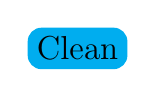
\begin{tikzpicture}\node [fill=cyan, rounded corners=5pt] {\large Clean};\end{tikzpicture}}
\def\WaferSemiClean{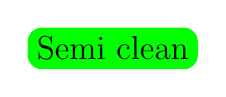
\begin{tikzpicture}\node [fill=green, rounded corners=5pt] {\large Semi clean};\end{tikzpicture}}
\def\WaferNonStandard{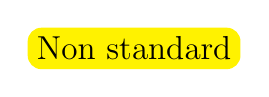
\begin{tikzpicture}\node [fill=yellow, rounded corners=5pt] {\large Non standard};\end{tikzpicture}}

\usepackage[colorlinks=true,linkcolor=blue,urlcolor=black,bookmarksopen=true]{hyperref}
\usepackage{bookmark}
\usepackage{hyperref}
\usepackage{sepfootnotes}
\usepackage{lipsum,tocloft} 
\usetikzlibrary{positioning}
\usetikzlibrary{patterns}

\usepackage[digital,srcmeas]{circdia}

\usepackage{float}
\floatstyle{boxed} 
\restylefloat{figure}

\title{Libre Silicon process specification}
\date{\today}
\author{David Lanzendörfer}
\makeindex

\newcounter{ct}
\def\CrossSectionOnly{0.3}
\def\CrossAndTopSection{0.2}
\def\CrossAndTopSectionBig{0.3}
\def\VLSILayout{0.4}

\DeclareMathOperator\erfc{erfc}

\setlength{\parindent}{0pt} % get rid of annoying indents

%\numberline{\thefootnotes}
%%#1

\newcommand{\listfootnotesname}{\section{List of Footnotes}}% 'List of Footnotes' title 
\newlistof[chapter]{footnotes}{fnt}{\listfootnotesname}% New 'List of...' for footnotes 
\let\oldfootnote\footnote % Save the old \footnote{...} command 
\renewcommand\footnote[1]{% Redefine the new footnote to also add 'List of Footnote' entries. 
	\refstepcounter{footnotes}% Add and step a reference to the footnote/counter. 
	\oldfootnote{#1}% Make a regular footnote
	\addcontentsline{fnt}{footnotes}{
		\protect
		\tiny{
			#1
			%\thefootnotes
		}
	}% Add the 'List of...' entry. 
}

\begin{document}
\maketitle

\begin{abstract}
	Copyright © 2017 LANCEVILLE TECHNOLOGY GROUP CO., LIMITED. All rights reserved. \\

	This process is licensed under the Libre Silicon public license; you can redistribute it and/or modify it under the terms of the Libre Silicon public license
	as published by the Libre Silicon alliance, either version 1 of the License, or (at your option) any later version.

	This design is distributed in the hope that it will be useful, but WITHOUT ANY WARRANTY; without even the implied warranty of MERCHANTABILITY or FITNESS FOR A PARTICULAR PURPOSE.
	See the Libre Silicon Public License for more details. \\

	This is the specification of the free silicon manufacturing standard for manufacturing the LibreSilicon standard logic cells\footnote{\url{https://github.com/chipforge/StdCellLib}} and related free technology nodes from the LibreSilicon project.

	For this initial revision 0.1 a gate-first approach has been chosen which led to the choice of polysilicon as the gate electrode material because of the simplicity of the gate alignment.
	For better isolation properties of the transistors and gates in overall a box-isolation approach has been chosen.
	All of these choices have been made with the future scale down from the recent $1 \mu m$ to smaller structure sizes.
	\textbf{This process is for manufacturing $1 \mu m$ only!}
	But further releases which will have been tested with smaller structure sizes can be expected.
\end{abstract}

\newpage
\tableofcontents
\newpage
\section{CMOS in a nutshell}
This basic initial project is dedicated to the CMOS Technology only and for this reason two types of metal–oxide–semiconductor field-effect transistors (MOSFET) are required.

Historicaly, the first chips with MOSFETs on the mass market were p-channel MOSFETs in enhancement-mode.

\begin{center}
	\begin{figure}[h]
		\begin{center}
			\begin{circuitdiagram}{20}{20}
				\power{15}{18.5}{U}{}  % power above pmos
				\wire{15}{18}{15}{16}   % wire above pmos
				\trans{penh}{13}{14}{R}{}{} % pmos -> right
				\Voltarrow{14}{18}{10}{16}{u}{$-V_{GS}$}
				\wire{15}{12}{15}{8}   % wire below pmos
				\resis{15}{5}{V}{$R_D$}{}  % resistor on drain
				\wire{15}{1}{15}{2}   % wire below pmos
				\ground{15}{0.5}{D}  % ground below resistor
				\othersrc[\sigsym{-rec}]{o}{5.5}{15.5}{H}{}{signal}
				\pin{9.5}{15.5}{R}{}	% pin in
				\ground{2.5}{0.5}{D}  % ground below signal source
				\wire{2.5}{1}{2.5}{15.5}   % wire below signal
				\junct{15}{10}   % dot
				\wire{15}{10}{16}{10}   % wire before out
				\pin{17}{10}{R}{out}	% pin out
			\end{circuitdiagram}
		\end{center}
		\caption{enhancement-mode PMOS transistor use-case}
	\end{figure}
\end{center}

The sectional view of a PMOS transistor in silicon is being shown below
\begin{center}
	\begin{tikzpicture}[node distance = 3cm, auto, thick,scale=0.5, every node/.style={transform shape}]
		% substrate
		\fill[YellowOrange] (0,0) rectangle (10,2);
		\node at (2,0.5) {Si (p-type)};

		% n-well
		\fill[Goldenrod] (1.25,0.75) rectangle (8.25,2);
		\node at (5.75,1) {N-Well};

		% body
		\fill[ProcessBlue] (1.5,1) rectangle (3,2);
		\node at (2,1.5) {n+};
		% source
		\fill[RedOrange] (3.5,1) rectangle (5,2);
		\node at (4,1.5) {p+};
		% drain
		\fill[RedOrange] (6.5,1) rectangle (8,2);
		\node at (7,1.5) {p+};
		%% gate:
		% gate oxide
		\fill[LightGray] (4.8,2) rectangle (6.7,2.1);
		% gate poly
		\fill[BrickRed] (4.8,2.1) rectangle (6.7,2.2);

		% metals ground
		\fill[DarkDarkGray] (2,2) rectangle (2.5,3);
		\fill[DarkDarkGray] (4,2) rectangle (4.5,3);
		\fill[DarkDarkGray] (1,3) rectangle (4.5,3.2); % connection pad GND

		\fill[DarkDarkGray] (5.5,2.2) rectangle (6,3);
		\fill[DarkDarkGray] (5.3,3) rectangle (6.2,3.2); % connection pad VG

		\fill[DarkDarkGray] (7,2) rectangle (7.5,3);
		\fill[DarkDarkGray] (6.8,3) rectangle (7.7,3.2); % connection pad VDD

		% isolation oxides:
		\fill[NormalGray] (1,2) rectangle (2,3);
		\fill[NormalGray] (2.5,2) rectangle (4,3);
		\fill[NormalGray] (4.5,2) rectangle (4.8,3);
		\fill[NormalGray] (4.8,2.2) rectangle (5.5,3);
		\fill[NormalGray] (6,2.2) rectangle (6.7,3);
		\fill[NormalGray] (6.7,2) rectangle (7,3);
		\fill[NormalGray] (7.5,2) rectangle (8.5,3);

		\node at (1.5,3.5) {Source};
		\node at (5.5,3.4) {Gate};
		\node at (7.5,3.4) {Drain};

		%field oxides:
		\fill[DarkGray] (0,2) rectangle (1,4);
		\fill[DarkGray] (8.5,2) rectangle (10,4);
		\fill[RedOrange] (0,1.5) rectangle (1,2);
		\node at (0.5,1.75) {p+};
		\fill[RedOrange] (8.5,1.5) rectangle (10,2);
		\node at (9.5,1.75) {p+};
	\end{tikzpicture}
\end{center}

Historicaly later, faster chips with MOSFETs on the mass market were marked as n-channel MOSFETs in enhancement mode also.

\begin{center}
	\begin{figure}[h]
		\begin{center}
			\begin{circuitdiagram}{20}{20}
				\power{15}{18.5}{U}{}  % power above resistor
				\wire{15}{17}{15}{18}   % wire above resistor
				\resis{15}{14}{V}{$R_D$}{}  % resistor on drain
				\wire{15}{11}{15}{8}   % wire between resistor and nmos
				\trans{nenh}{13}{6}{R}{}{} % nmos -> right
				\Voltarrow{10}{4}{14}{1}{d}{$+V_{GS}$}
				\wire{15}{1}{15}{4}   % wire below nmos
				\ground{15}{0.5}{D}  % ground below nmos
				\othersrc[\sigsym{rec}]{o}{5.5}{4.5}{H}{}{signal}
				\pin{9.5}{4.5}{R}{}	% pin in
				\ground{2.5}{0.5}{D}  % ground below signal source
				\wire{2.5}{1}{2.5}{4.5}   % wire below signal
				\junct{15}{10}   % dot
				\wire{15}{10}{16}{10}   % wire before out
				\pin{17}{10}{R}{out}	% pin out
			\end{circuitdiagram}
		\end{center}
		\caption{enhancement-mode NMOS transistor use-case}
	\end{figure}
\end{center}

The sectional view of a NMOS transistor in silicon is being shown here also.
\begin{center}
	\begin{tikzpicture}[node distance = 3cm, auto, thick,scale=0.5, every node/.style={transform shape}]
		% substrate
		\fill[YellowOrange] (0,0) rectangle (10,2);
		\node at (2,0.5) {Si (p-type)};
		% body
		\fill[RedOrange] (1.5,1) rectangle (3,2);
		\node at (2,1.5) {p+};
		% source
		\fill[ProcessBlue] (3.5,1) rectangle (5,2);
		\node at (4,1.5) {n+};
		% drain
		\fill[ProcessBlue] (6.5,1) rectangle (8,2);
		\node at (7,1.5) {n+};
		%% gate:
		% gate oxide
		\fill[LightGray] (4.8,2) rectangle (6.7,2.1);
		% gate poly
		\fill[BrickRed] (4.8,2.1) rectangle (6.7,2.2);
		% metals ground
		\fill[DarkDarkGray] (2,2) rectangle (2.5,3);
		\fill[DarkDarkGray] (4,2) rectangle (4.5,3);
		\fill[DarkDarkGray] (1,3) rectangle (4.5,3.2); % connection pad GND

		\fill[DarkDarkGray] (5.5,2.2) rectangle (6,3);
		\fill[DarkDarkGray] (5.3,3) rectangle (6.2,3.2); % connection pad VG

		\fill[DarkDarkGray] (7,2) rectangle (7.5,3);
		\fill[DarkDarkGray] (6.8,3) rectangle (7.7,3.2); % connection pad VDD

		% isolation oxides:
		\fill[NormalGray] (1,2) rectangle (2,3);
		\fill[NormalGray] (2.5,2) rectangle (4,3);
		\fill[NormalGray] (4.5,2) rectangle (4.8,3);
		\fill[NormalGray] (4.8,2.2) rectangle (5.5,3);
		\fill[NormalGray] (6,2.2) rectangle (6.7,3);
		\fill[NormalGray] (6.7,2) rectangle (7,3);
		\fill[NormalGray] (7.5,2) rectangle (8.5,3);

		%field oxides:
		\fill[DarkGray] (0,2) rectangle (1,4);
		\fill[DarkGray] (8.5,2) rectangle (10,4);
		\fill[RedOrange] (0,1.5) rectangle (1,2);
		\node at (0.5,1.75) {p+};
		\fill[RedOrange] (8.5,1.5) rectangle (10,2);
		\node at (9.5,1.75) {p+};

		\node at (1.5,3.5) {Source};
		\node at (5.5,3.4) {Gate};
		\node at (7.5,3.4) {Drain};
	\end{tikzpicture}
\end{center}

Both technologies, the older NMOS as the newer PMOS, have the same disadvantage. Every time, the transistor is switched on, the current between Drain and Source of the transistor is limited by the Resistor on Drain only. Higher currents here meaning also higher power consumption for the chip where the transistors are integrated also. If the transistors are switched off, now currents flows between Drain and Source anymore, the power consumption of the chip also goes low.
Et violà, the US-Patent with Number 3356858\footnote{https://www.google.com/patents/US3356858} changed the world and combines both technologies to the new complementary metal-oxide-semiconductor (CMOS) technology. Instead of every transistor is working against a weak resistor, the transistor works against a complementary switched-off transistor. With the Eyes of our antecessor CMOS doubles the transistor count, but contemporary chips all are build in CMOS.

\begin{center}
	\begin{figure}[h]
		\begin{center}
			\begin{circuitdiagram}{20}{20}
				\power{15}{18.5}{U}{}  % power above pmos 
				\wire{15}{16}{15}{18}   % wire above pmos
				\trans{penh}{13}{14}{R}{}{} % pmos -> right
				\Voltarrow{14}{18}{10}{16}{u}{$-V_{GS}$}
				\wire{15}{8}{15}{12}   % wire between pmos and nmos
				\trans{nenh}{13}{6}{R}{}{} % nmos -> right
				\Voltarrow{10}{4}{14}{1}{d}{$+V_{GS}$}
				\wire{15}{1}{15}{4}   % wire below nmos
				\ground{15}{0.5}{D}  % ground below nmos
				\othersrc[\sigsym{rec}]{o}{5}{10}{H}{}{signal}
				\pin{9}{10}{R}{}	% pin in
				\wire{9.5}{10}{10}{10}   % wire before gates
				\wire{10}{15.5}{10}{4.5}   % wire between gates
				\junct{10}{10}   % dot
				\ground{2}{0.5}{D}  % ground below signal source
				\wire{2}{1}{2}{10}   % wire below signal
				\junct{15}{10}   % dot
				\wire{15}{10}{16}{10}   % wire before out
				\pin{17}{10}{R}{out}	% pin out
			\end{circuitdiagram}
		\end{center}
		\caption{complementary PMOS and NMOS transistor couple use-case}
	\end{figure}
\end{center}

Below the sectional view of the inverter circuitry can be seen.
For the run through of this process we will use this cross section diagram as reference.
\begin{center}
	\begin{tikzpicture}[node distance = 3cm, auto, thick,scale=0.6, every node/.style={transform shape}]
		% substrate
		\fill[YellowOrange] (0,0) rectangle (20,2);
		\node at (2,0.5) {Si (p-type)};
		% n-well
		\fill[Goldenrod] (1.25,0.75) rectangle (8.25,2);
		\node at (5.75,1) {N-Well};
		% body
		\fill[ProcessBlue] (1.5,1) rectangle (3,2);
		\node at (2,1.5) {n+};
		% source
		\fill[RedOrange] (3.5,1) rectangle (5,2);
		\node at (4,1.5) {p+};
		% drain
		\fill[RedOrange] (6.5,1) rectangle (8,2);
		\node at (7,1.5) {p+};
		%% gate:
		% gate oxide
		\fill[LightGray] (4.8,2) rectangle (6.7,2.1);
		% gate poly
		\fill[BrickRed] (4.8,2.1) rectangle (6.7,2.2);
		% isolation oxides:
		\fill[NormalGray] (1,2) rectangle (2,3);
		\fill[NormalGray] (2.5,2) rectangle (4,3);
		\fill[NormalGray] (4.5,2) rectangle (4.8,3);
		\fill[NormalGray] (4.8,2.2) rectangle (5.5,3);
		\fill[NormalGray] (6,2.2) rectangle (6.7,3);
		\fill[NormalGray] (6.7,2) rectangle (7,3);
		\fill[NormalGray] (7.5,2) rectangle (8.5,3);

		%field oxides:
		\fill[DarkGray] (0,2) rectangle (1,4);
		\fill[DarkGray] (8.5,2) rectangle (11.5,4);
		\fill[DarkGray] (19,2) rectangle (20,4);

		\fill[RedOrange] (0,1.5) rectangle (1,2);
		\fill[RedOrange] (8.5,1.5) rectangle (11.5,2);
		\fill[RedOrange] (19,1.5) rectangle (20,2);

		\node at (0.5,1.75) {p+};
		\node at (9.5,1.75) {p+};
		\node at (19.5,1.75) {p+};

		%%% nmos:
		% body
		\fill[RedOrange] (17,1) rectangle (18.5,2);
		\node at (18,1.5) {p+};
		% source
		\fill[ProcessBlue] (15,1) rectangle (16.5,2);
		\node at (16,1.5) {n+};
		% drain
		\fill[ProcessBlue] (12,1) rectangle (13.5,2);
		\node at (13,1.5) {n+};

		%% gate:
		% gate oxide
		\fill[LightGray] (13.3,2) rectangle (15.2,2.1);
		% gate poly
		\fill[BrickRed] (13.3,2.1) rectangle (15.2,2.2);

		% metals
		\fill[DarkDarkGray] (17.5,2) rectangle (18,3);
		\fill[DarkDarkGray] (15.5,2) rectangle (16,3);
		\fill[DarkDarkGray] (15.5,3) rectangle (19,3.2); % connection pad GND

		\fill[DarkDarkGray] (14,2.2) rectangle (14.5,3);
		\fill[DarkDarkGray] (13.8,3) rectangle (14.7,3.2); % connection pad VG

		\fill[DarkDarkGray] (12.5,2) rectangle (13,3);
		\fill[DarkDarkGray] (12.3,3) rectangle (13.2,3.2); % connection pad VDD

		\fill[DarkDarkGray] (2,2) rectangle (2.5,3);
		\fill[DarkDarkGray] (4,2) rectangle (4.5,3);
		\fill[DarkDarkGray] (1,3) rectangle (4.5,3.2); % connection pad GND

		\fill[DarkDarkGray] (5.5,2.2) rectangle (6,3);
		\fill[DarkDarkGray] (5.3,3) rectangle (6.2,3.2); % connection pad VG

		\fill[DarkDarkGray] (7,2) rectangle (7.5,3);
		\fill[DarkDarkGray] (6.8,3) rectangle (7.7,3.2); % connection pad VDD

		% isolation oxides:
		\fill[NormalGray] (18,2) rectangle (19,3);
		\fill[NormalGray] (16,2) rectangle (17.5,3);
		\fill[NormalGray] (15.2,2) rectangle (15.5,3);
		\fill[NormalGray] (14.5,2.2) rectangle (15.2,3);
		\fill[NormalGray] (13.3,2.2) rectangle (14,3);
		\fill[NormalGray] (13,2) rectangle (13.3,3);
		\fill[NormalGray] (11.5,2) rectangle (12.5,3);

		\node at (1.5,3.5) {VDD};
		\node at (16.5,3.5) {Ground};
		\node at (5.5,3.4) {Input};
		\node at (14,3.4) {Input};
		\node at (7,3.4) {Output};
		\node at (12.5,3.4) {Output};

		\node at (0.5,4.2) {Field oxide};
		\node at (9.5,4.2) {Field oxide};
		\node at (19.5,4.2) {Field oxide};
	\end{tikzpicture}
\end{center}
\newpage
\section{Physics}
In this chapter we deal with all the physics related to solid state device manufacturing.
In case there is anything unclear, please look up this chapter and its sub-chapters.
\section{Getting doping from resistance}
In many cases the supplier will only provide the resistance per length specification for their substrate and won't give you the dopant concentration numbers.
In this case you will have to find these numbers out yourself by converting it from the numbers they've provided.

\begin{figure}[H]
	\centering
	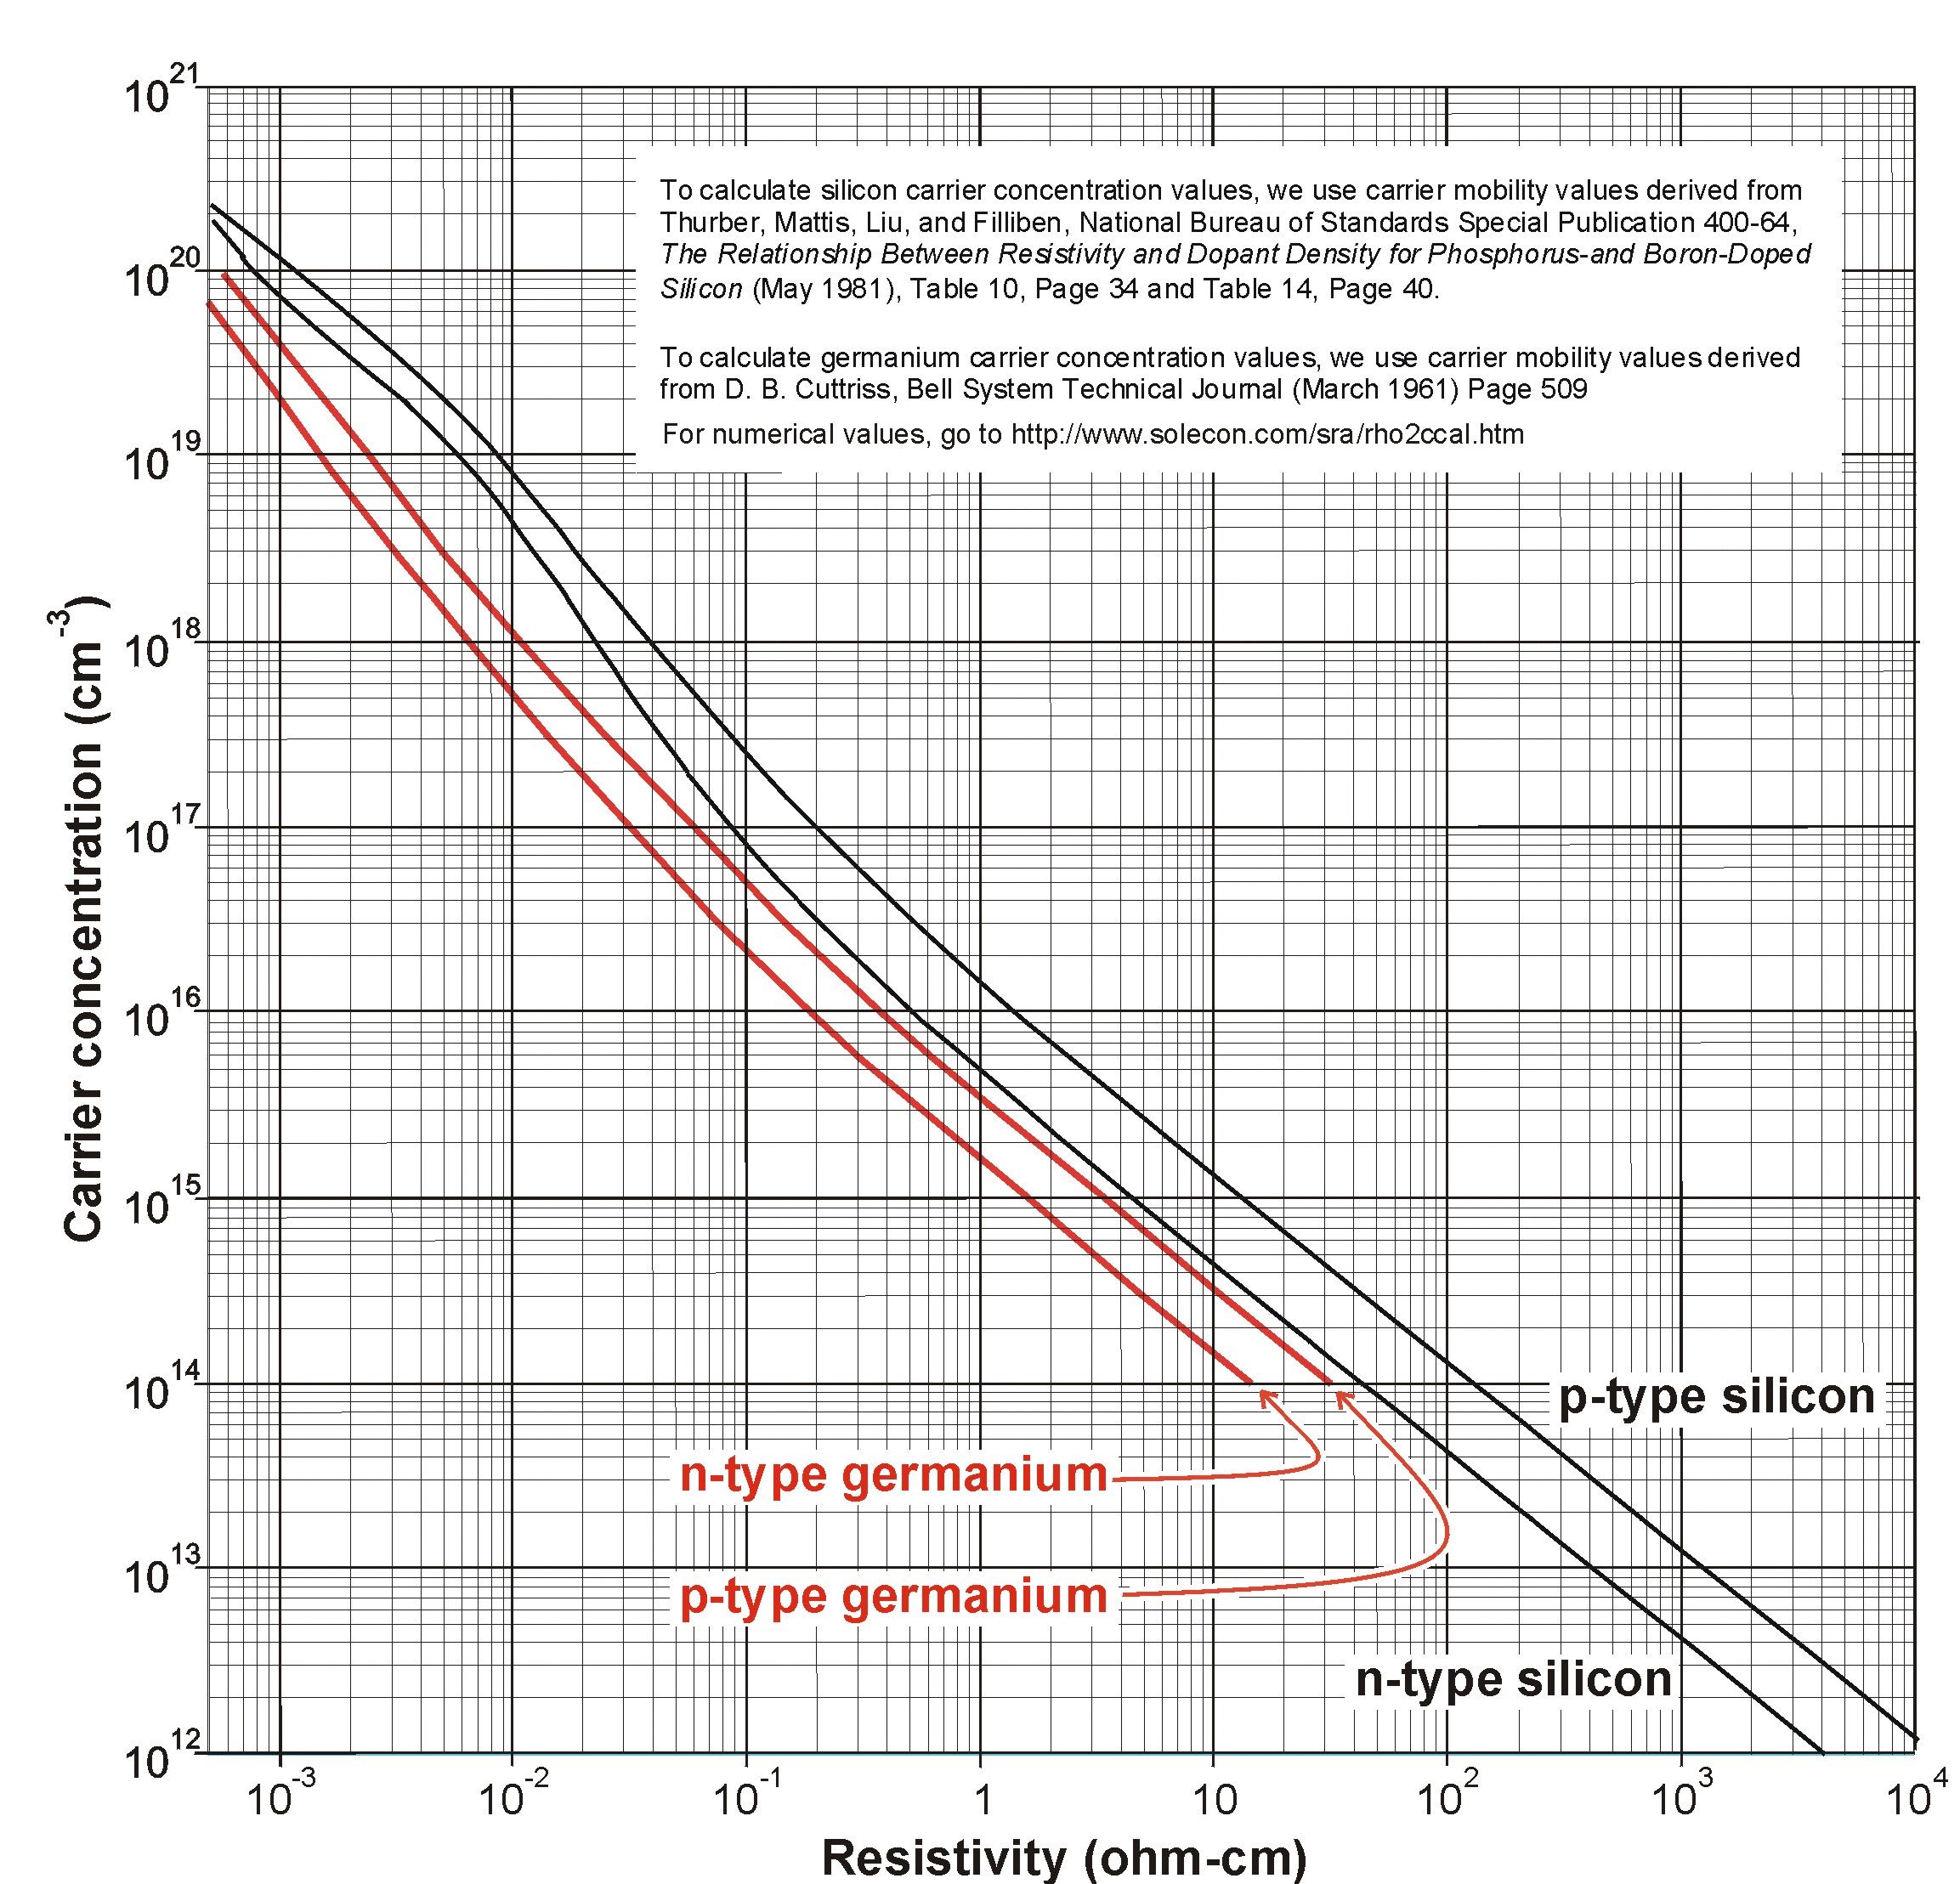
\includegraphics[width=0.5\textwidth]{resistance_doping.png}
	\caption{R-L-dopant relation}
	\label{r_l_nd_relation}
\end{figure}

You can either use the graphics from \autoref{r_l_nd_relation} and determine the dopant concentration graphically, which is very very imprecise or use a online tool like the one from Solecon\footnote{\url{http://www.solecon.com/sra/rho2ccal.htm}}

Germanium is being included in this graphics just in case someone is going to fork this process based on Germanium substrate.
\newpage
\subsection{Infusion}
The redistribution process depends on the ratio of the solubility of the doping material in silicon and SiO$ _2$. At the Si/SiO$ _2$ interface the dopants are redistributed by segregation until the ratio of their concentration at the interface is the same as the ratio of their solubility in both materials. The ratio of dopant solubility is expressed by the segregation coefficient $m$ which is

\begin{equation}
\displaystyle m = \frac{
	\mathrm{solubility\ in\ silicon}
	}{
	\mathrm{solubility\ in\ SiO_2}
	}
\end{equation}

As listed in \autoref{table_diffusion_coeff} below there are dopant species which solubilize better in SiO$ _2$ than in silicon ($ m < 1$) and species which have a reversed behavior ($ m > 1$).
In case of $ m < 1$, as for Boron, the dopant concentration is enhanced at the SiO$ _2$ side, whereas beneath the interface, there is a dopant depletion at the silicon surface.
For reversed solubility ratios ($ m > 1$, like Phosphorus), only few dopant atoms penetrate the interface.
In order to obtain the by $ m$ determined concentration ratio at the interface, dopant atoms from deeper silicon zones diffuse back to the surface zone.
Therefore, the dopant concentration at the silicon surface is enhanced, as illustrated in \autoref{graph_figure}b.
In \autoref{graph_figure} $ C_c$ denotes the dopant concentration in the silicon surface zone before oxidation. $ x$ is the distance from the silicon surface.

\begin{figure}[H]
	\centering
	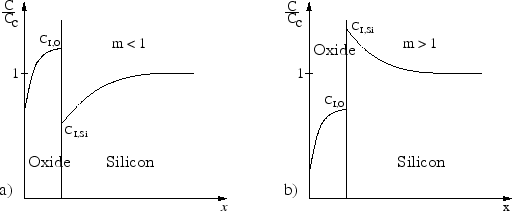
\includegraphics[width=0.75\linewidth]{img349.png}
	\caption{Schematic illustration of dopant redistribution}
	\label{graph_figure}
\end{figure}
\begin{table}[H]
	\centering
	\begin{tabular}{|c|c|c|c|c|c|}
		\hline
		Dopant species &
		Boron &
		Phosphor &
		Antimon &
		Arsen &
		Gallium \\
		\hline
		$m$ &
		0.1-0.3 &
		10 &
		10 &
		10 &
		20 \\
		\hline
	\end{tabular}
	\caption{Segregation coefficients $m$ for important dopant species in silicon}
	\label{table_diffusion_coeff}
\end{table}
\newpage
\subsection{Constant source diffusion (Predeposition)}

Although the diffusion process of donors and acceptors into the silicon crystal is a three dimensional process for simplicity we first only discuss the one dimensional mathematics for it in order to get a "simple" equation for the depth-time-temperature relation.

\begin{mdframed}[linewidth=2pt,linecolor=red]
This is only valid for a constant source of dopants on the surface of the wafer (for instance gas).
These equations are being used for predicting the pre-deposition step (in case this process would be adapted by someone for predeposition instead of ion implant)
\end{mdframed}

We start with Ficks law (for all German speakers: Yes that's his name, not me shouting about this problem) where the dopant concentration N is coupled with time and place
\begin{equation}
\frac{\partial N}{\partial t} = D \cdot \frac{\partial^2 N}{\partial x^2}
\end{equation}

The diffusion coefficient is as well material as well as temperature dependent  and can be calculated with the following equation:
\begin{equation}
D = D_0 \cdot \exp\left(-\frac{E_a}{k \cdot T}\right)
\end{equation}
With $k=8.62 \cdot 10^{-5} \frac{eV}{K}$ being the Boltzman constant and in \autoref{absolute_diffusion_coefficients} we can see the $D_0$ and $E_a$ values for the most common materials\footnote{ISBN 3-8023-1588:Hoppe Bernhard, Mikroelektronik 2, Page 24, Table 2.1} which we can use within the further calculations for our well dimensioning phases. The temperature usually is in the area of $1000\degree C$ or in Kelvin $1273.15\degree K$.
\begin{table}[H]
	\centering
	\begin{tabular}{|c|c|c|}
		\hline
		Element &
		$D_0$ $\left[\frac{cm^2}{s}\right]$ &
		$E_a$ $\left[eV\right]$ \\
		\hline
		P &
		10.50 &
		3.69 \\
		\hline
		As &
		0.32 &
		3.56 \\
		\hline
		Sb &
		5.60 &
		3.95 \\
		\hline
		B &
		10.50 &
		3.69 \\
		\hline
		Al &
		8.00 &
		3.47 \\
		\hline
		Ga &
		3.60 &
		3.51 \\
		\hline
		Cu &
		0.0025 &
		0.65 \\
		\hline
	\end{tabular}
	\label{absolute_diffusion_coefficients}
	\caption{$D_0$ and $E_a$ values for Boron and Phosphorus}
\end{table}

The law stated above
\begin{equation}
\frac{\partial N}{\partial t} = D \cdot \frac{\partial^2 N}{\partial x^2} 
\end{equation}
has the same form as the temperature conductivity equation (Laplace) for which we already have a general solution
\begin{equation}
\frac{\partial u}{\partial t} = a^2 \cdot \frac{\partial^2 u}{\partial x^2} 
\end{equation}

Which means that we can map the general solution for the temperature conductivity equations after Laplace
\begin{equation}
u(x,t) = \frac{1}{2 \cdot a \cdot \sqrt{\pi \cdot t}} \cdot \int_{-\infty}^{\infty}{f(a)\cdot\exp\left(\frac{-(x-a)^2}{4 \cdot a^2 \cdot t^2}\right)}da
\end{equation}
to our Ficks law with $a=\sqrt{D}$ und $u=N$
\begin{equation}
N(x,t) = \frac{1}{2 \cdot \sqrt{D} \cdot \sqrt{\pi \cdot t}} \cdot \int_{-\infty}^{\infty}{f(\sqrt{D})\cdot\exp\left(\frac{-(x-\sqrt{D})^2}{4 \cdot D \cdot t^2}\right)}da
\end{equation}
with the edge conditions
\begin{equation}
N( x=0 , t > 0 ) = N_0
\end{equation}
\begin{equation}
N( x \geq 0 ,  t = 0 ) = 0
\end{equation}
we get the resulting function from the solving process for the Laplace temperature conduction equations
\begin{equation}
u(x,t)=u_0 \cdot erfc\left(\frac{x}{2 \cdot a \cdot \sqrt{t}}\right)
\end{equation}
with the error function being an integral of the form
\begin{equation}
erfc(z)
=
\left(1-\frac{2}{\sqrt{\pi}}\right)\cdot\int_0^z{e^{-a^2}}da
\end{equation}

Or in case of our dopant concentration equation we can replace a with the square root of the diffusion coefficient in order to get the error function for our dopant density euqtion:
\begin{equation}
erfc(z)
=
\left(1-\frac{2}{\sqrt{\pi}}\right)\cdot\int_0^z{e^{-D}}d\sqrt{D}
\end{equation}
\begin{equation}
N(x,t)
=
N_0 \cdot erfc\left(\frac{x}{2 \cdot \sqrt{D \cdot t}}\right)
=
N_0 \cdot erfc\left(\frac{x}{x_l(t)}\right)
\end{equation}
Now we can extract the layer thickness respectively the depth of the well in dependency of the time and the temperature:
\begin{equation}
x_l(t) = 2 \cdot \sqrt{D \cdot t}
\end{equation}
\begin{equation}
x_l(t) = 2 \cdot \sqrt{D_0 \cdot \exp\left(-\frac{E_a}{k \cdot T}\right) \cdot t}
\end{equation}

And plot the result for multiple different drive in times
\begin{figure}[H]
	\centering
	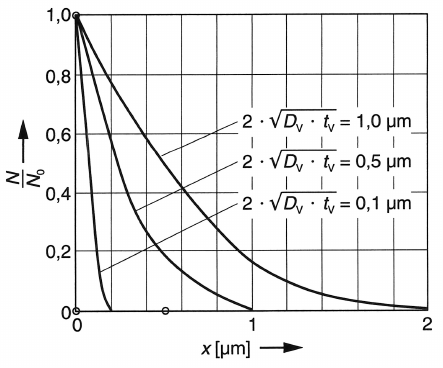
\includegraphics[scale=0.5]{dopants_depth.png}
	\caption{Different predeposition times}
\end{figure}

We can now describe the dosage based on the time and temperature of the diffusion

\begin{equation}
Q=\frac{2}{\sqrt{\pi}} \cdot N_0 \cdot \sqrt{D \cdot t}
\end{equation}

Where $N_0$ (concentration at the surface) equals the maximum solubility of a given element (e.g. Boron) within the given medium (e.g. Silicon).

\newpage
\subsection{Ion implant}
We can use the following equation to calculate the carrier distribution after implantation:
\begin{equation}
N(x,t)
=
N_p \exp\left(-\frac{(x-R_p)^2}{2\Delta R_p^2}\right)
=
\frac{Q}{\sqrt{2\pi}\Delta R_p}\exp\left(-\frac{(x-R_p)^2}{2\Delta R_p^2}\right)
\end{equation}

Where the projected range ($R_p$) and the projected straggle ($\Delta R_p$) need to be looked up in tables or looked up using an online tool like the one linked in the footnote\footnote{\url{http://cleanroom.byu.edu/rangestraggle}}
\subsection{Diffusion (Drive-in)}

\subsection{Vertical diffusion and junction formation (Well formation)}\label{building_wells}
The goal of most diffusions is to form pn junctions by converting p-type material to n-type material or vice versa.
In \autoref{junction_formation_plot}, for example, the wafer is uniformly doped n-type material with a concentration indicated by $N_B$, and the diffusing impurity is boron.
The point at which the diffused impurity profile intersects the background concentration is the mettalurgical junction depth ($x_j$).
The net impurity concentration at $x_j$ is zero.
Setting $N(x)$ equal to the background concentration $N_B$ at $x=x_j$ yields\footnote{Gerold W. Neudeck and Robert F. Pierret, Modular series on solid state devices, Volume V, Chapter 4}
\begin{equation}
x_j
=
2 \cdot\sqrt{D \cdot t \cdot \ln\left(\frac{N_0}{N_B}\right)}
\end{equation}
and
\begin{equation}
x_j
=
2 \cdot\sqrt{D \cdot t}
\cdot
\erfc^{-1}\left(\frac{N_B}{N_0}\right)
\end{equation}

for the Gaussian and complementary error function distributions, respectively.

In \autoref{junction_formation_plot}, the boron concentration $N$ exceeds $N_B$ to the left of the junction, and this region is p-type.
To the right of $x_j$, $N$ is less than $N_B$, and this region remains n-type.

To calculate the junction depth, we must know the background concentration $N_B$ of the original wafer.
Look at \autoref{r_l_nd_relation} for this purpose.

\begin{figure}[H]
	\centering
	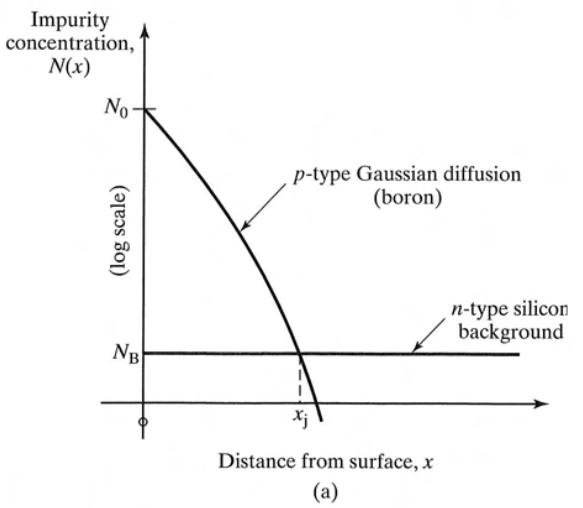
\includegraphics[scale=0.5]{well_formation1.png}
	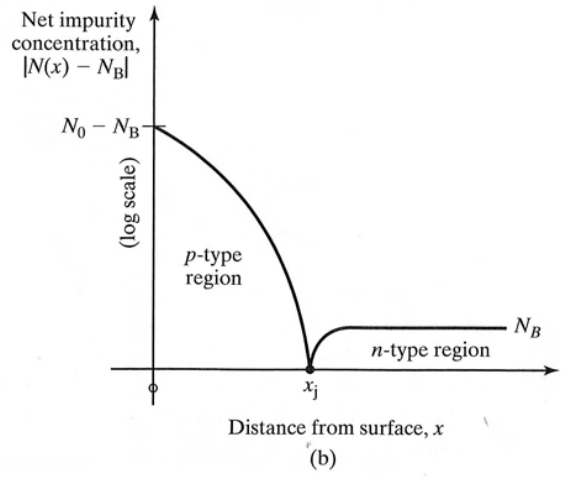
\includegraphics[scale=0.5]{well_formation2.png}
	\caption{Formation of a pn junction by diffusion: (a) An example of a p-type Gaussian diffusion into a uniformly doped n-type wafer; (b) net impurity concentration in the wafer.}
	\label{junction_formation_plot}
\end{figure}


\newpage
\section{MOS Capacitance}
\url{https://ecee.colorado.edu/~bart/book/book/chapter6/ch6_3.htm}

\subsection{Threshold voltage with metal gate ($V_T$)}
$V_{FB}$ is the flat band voltage and is given by:
\begin{equation}
V_{FB}
=
\phi_{MS} - \frac{Q_{SS}}{C_{ox}}
=
\phi_{M} - \phi_{S} - \frac{Q_{SS}}{C_{ox}}
\end{equation}

With
\begin{equation}
\phi_{S}
=
\chi + \frac{E_g}{2 q} + \phi_F 
\end{equation}
we get
\begin{equation}
V_{FB}
=
\phi_{M} -  \left(\chi + \frac{E_g}{2 q} + \phi_F \right) - \frac{Q_{SS}}{C_{ox}}
\end{equation}

And because of the simplifications we did to $F_{FB}$ we get to:
\begin{equation}
V_T = 2 \phi_F + \frac{2 \sqrt{\epsilon_{Si}\cdot q\cdot \left| \phi_F \right| \cdot N }}{C_{ox}} + V_{FB}
\end{equation}
\begin{equation}
V_T = 2 \phi_F + \frac{2 \sqrt{\epsilon_{Si}\cdot q\cdot \left| \phi_F \right| \cdot N }}{C_{ox}} + \phi_{M} -  \left(\chi + \frac{E_g}{2 q} + \phi_F \right) - \frac{Q_{SS}}{C_{ox}}
\end{equation}
\begin{equation}
V_T = 2 \phi_F + \frac{2 \sqrt{\epsilon_{Si}\cdot q\cdot \left| \phi_F \right| \cdot N }}{C_{ox}} + \phi_{M} -  \chi - \frac{E_g}{2 q} - \phi_F - \frac{Q_{SS}}{C_{ox}}
\end{equation}
\begin{equation}
V_T = \phi_F + \frac{2 \sqrt{\epsilon_{Si}\cdot q\cdot \left| \phi_F \right| \cdot N }}{C_{ox}} + \phi_{M} -  \chi - \frac{E_g}{2 q} - \frac{Q_{SS}}{C_{ox}}
\end{equation}

The contact potential from the Aluminum contact to the surface of the gate (silicon below the oxide) is fixed for $T=300\degree K$:
\begin{equation}
\phi_{M} -  \chi - \frac{E_g}{2 q} = 4.1V - 4.05V - \frac{1.12eV}{2 q} = 4.1V - 4.05V - 0.56V = -0.51V
\end{equation}

From that we get
\begin{equation}
V_T = \phi_F + \frac{2 \sqrt{\epsilon_{Si}\cdot q \cdot \left| \phi_F \right| \cdot N }}{C_{ox}} - 0.51V
\end{equation}

Now we can calculate the thresholds for P substrate ($V_{Tp}$) and N substrate  ($V_{Tn}$), respectively the wells we build on unpredoped substrated, which makes the equation for single-doped substrate valid for both wells with

Which brings us to the equations for the N-channel and P-channel thresholds:

(N-Channel MOSFETs are built on p-substrate)
\begin{equation}
V_{Tn} = \phi_{Fp} + \frac{2 \sqrt{\epsilon_{Si}\cdot q \cdot \left| \phi_{Fp} \right| \cdot N}}{C_{ox}} - 0.51V
\end{equation}

(P-Channel MOSFETs are built on n-substrate)
\begin{equation}
V_{Tp} = \phi_{Fn} + \frac{2 \sqrt{\epsilon_{Si}\cdot q \cdot \left| \phi_{Fn} \right| \cdot N}}{C_{ox}} - 0.51V
\end{equation}

This equation will be used further on to find the optimum gate oxide thickness for our transistors.



\subsubsection{Threshold voltage with poly silicon gate ($V_T$)}
The formula for calculating the threshold voltage of a MOS device is the following:
\begin{equation}
V_T = V_{t-mos} + V_{FB}
\end{equation}
where $V_{t-mos}$ is the threshold voltage of an ideal MOS capacitor, $V_{FB}$ is the flat-band voltage and $V_{t-mos}$ is the threshold.
The MOS threshold voltage, $V_{t-mos}$ is calculated by considering the MOS capacitor structure that form the gate of the MOS transistor.

The ideal threshold voltage may be expressed as:
\begin{equation}
V_{t-mos}=2 \phi_F + \frac{Q_b}{C_{ox}}
\end{equation}
\begin{equation}
Q_b
=
\sqrt{2 \epsilon_{Si} \cdot q \cdot N  \cdot  ( \left| 2 \phi_F \right| + V_{SB}) }
\end{equation}
where $C_{ox}$ is the oxide capacitance and $Q_b$ which is called the bulk charge term.\\

Since we connect bulk and source $V_{SB}=0$ we can simplify the equation to become
\begin{equation}
Q_b
=
\sqrt{2\cdot\epsilon_{Si}\cdot q\cdot N \cdot  ( \left| 2 \cdot \phi_F \right|) }
\end{equation}
\begin{equation}
Q_b
=
2\cdot\sqrt{\epsilon_{Si}\cdot q\cdot N \cdot \left| \phi_F \right| }
\end{equation}


$V_{FB}$ is the flat band voltage and is given by:
\begin{equation}
V_{FB}
=
\phi_{MS}-\frac{Q_{SS}}{C_{ox}}-\frac{1}{C_{ox}}\int_{0}^{t_{ox}}\frac{x}{x_{ox}}\rho(x) dx
\end{equation}

Because we're not yet dealing with non-volatile memory devices which contain an oxide surface state charge we can just $\rho(x)=0$.
$Q_{SS}$ is a value which has to be measured.

\begin{equation}
V_{FB}
=
\phi_{MS} - \frac{Q_{SS}}{C_{ox}}
\end{equation}
with
\begin{equation}
V_{FB}
=
\phi_{MS} - \frac{Q_{SS}}{C_{ox}}
=
\phi_{M} - \phi_{S} - \frac{Q_{SS}}{C_{ox}}
\end{equation}

The term $\phi_{MS}$ is the work function difference between the gate material and the silicon substrate ($\phi_{gate}-\phi_{Si}$), which may be calculated for an n+ gate over a p substrate

\begin{equation}
\phi_{MSp}
=
-(\frac{E_g}{2}+\phi_{Fp})
\end{equation}

and for an n+ poly gate on an n-substrate
\begin{equation}
\phi_{MSn}
=
-(\frac{E_g}{2}-\phi_{Fn})
\end{equation}

Now we can calculate the thresholds for P substrate ($V_{Tp}$) and N substrate  ($V_{Tn}$), respectively the wells we build on unpredoped substrated, which makes the equation for single-doped substrate valid for both wells.

(N-Channel MOSFETs are built on p-substrate)
\begin{equation}
V_{Tn} = 2 \cdot \phi_{Fp} + \frac{2 \sqrt{\epsilon_{Si}\cdot q \cdot \left| \phi_{Fp} \right| \cdot N_p}}{C_{ox}} + \phi_{MSp} - \frac{Q_{SS}}{C_{ox}}
\end{equation}
\begin{equation}
V_{Tn} = 2 \cdot \phi_{Fp} + \frac{2 \sqrt{\epsilon_{Si}\cdot q \cdot \left| \phi_{Fp} \right| \cdot N_p}}{C_{ox}} -\frac{E_g}{2} - \phi_{Fp} - \frac{Q_{SS}}{C_{ox}}
\end{equation}
\begin{equation}
V_{Tn} = \phi_{Fp} + \frac{2 \sqrt{\epsilon_{Si}\cdot q \cdot \left| \phi_{Fp} \right| \cdot N_p}}{C_{ox}} -\frac{E_g}{2} - \frac{Q_{SS}}{C_{ox}}
\end{equation}

(P-Channel MOSFETs are built on n-substrate)
\begin{equation}
V_{Tp} = 2 \cdot \phi_{Fn} + \frac{2 \sqrt{\epsilon_{Si}\cdot q \cdot \left| \phi_{Fn} \right| \cdot N_n}}{C_{ox}} + \phi_{MSn} - \frac{Q_{SS}}{C_{ox}}
\end{equation}
\begin{equation}
V_{Tp} = 2 \cdot \phi_{Fn} + \frac{2 \sqrt{\epsilon_{Si}\cdot q \cdot \left| \phi_{Fn} \right| \cdot N_n}}{C_{ox}} -\frac{E_g}{2} + \phi_{Fn} - \frac{Q_{SS}}{C_{ox}}
\end{equation}
\begin{equation}
V_{Tp} = 3 \cdot \phi_{Fn} + \frac{2 \sqrt{\epsilon_{Si}\cdot q \cdot \left| \phi_{Fn} \right| \cdot N_n}}{C_{ox}} -\frac{E_g}{2} - \frac{Q_{SS}}{C_{ox}}
\end{equation}

This equation will be used further on to find the optimum gate oxide thickness for our transistors.



\section{Threshold voltage ($V_T$) adjustment}
At some point in the future this will be of very high relevance, because the lower the size of the transistors becomes, the higher the offset to $V_{Tp}$ and $V_{Tn}$ needs to be in order to stay on TTL 5V logic level, or at least compensate for the lowered voltages in order to reach the 3.3V CMOS logic levels.

Adjustment of the threshold voltage can be achieved by:
\begin{itemize}
\item A relatively small dose $N_I$ (units: ions/$cm^2$) of dopant atoms is implanted into the near-surface  region of the semiconductor.
\item When the MOS device is biased in depletion or inversion, the implanted dopants add to (or substract from) the depletion charge near the oxide-semiconductor interface
\end{itemize}

The formula to calculate the voltage offset is:
\begin{equation}
\Delta V_T = -\frac{q N_I}{C_{ox}} 
\left\{\begin{matrix}
N_I > 0\ for\ donor\ atoms\ (Phosporus/N) \\
N_I < 0\ for\ acceptor\ atoms\ (Boron/P)
\end{matrix}\right.
\end{equation}

\newpage
\section{Chemistry}
\subsection{Etching silicon dioxide}
A very "selective" chemical for SiO2 - i.e. does not etch silicon at all - is hydrofluoric acid (HF). If used directly such etchant has a too fast and aggresive action on the oxide, making very difficult the undercut and the linewidth control. For such reason, HF is universally used as a "buffered" solution, which can keep the etch rate low and constant, by moderating the PH level of the bath. This allows the etching time to be reliably correlated to the etching depth.

The industry standard buffered hydrofluoric acid solution (BHF\label{BHF}) has the following formulation:
\begin{itemize}
	\item 6 volumes of ammonium floride (NH4F, 40\% solution)
	\item 1 volume of HF.
\end{itemize}
This can be prepared, for example, by mixing 113 g of NH4F in 170 ml of H2O, and adding 28 ml of HF.\\
The etch rate at room temperature can range from 1000 to 2500 Å/min (100-250nm/min).
This depends on the actual density of the oxide which, as an amorphous layer, can have a more compact structure (if thermally grown in is oxygen) or less compact (if grown by CVD).
The following etching reaction holds:
\begin{equation}
	SiO_2 + 6HF \rightarrow H_2SiF_6 + H_2O
\end{equation}\\
where $H_2SiF_6$ is water soluble.\\
A common buffered oxide etch solution comprises a 6:1 volume ratio of 40\% NH4F in water to 49\% HF in water. This solution will etch thermally grown oxide at approximately 2 nanometres per second at 25 degrees Celsius.\label{BHF_six_to_one}
\footnote{Wolf, S.; R.N. Tauber (1986). Silicon Processing for the VLSI Era: Volume 1 - Process Technology. pp. 532–533. ISBN 978-0-9616721-3-3} \\

Another popular etching formulation is the P-etch:

60 volumes of $H_2O$ + 3 vol. of HF + 2 vol. of $HNO_3$, that is: 300 ml of $H_2O$ + 15 ml of HF + 10 ml of $HNO_3$.

The P-etch action is strongly dependent on oxide density, as it results from the growth technique.
An example is reported in the literature\footnote{A. Pliskin, J.Vac.Sci Technol., vol. 14, p.1064, 1977}, indicating 120 Å/min for thermal oxide and 250-700 Å/min for sputtered oxide.

A slow etching bath is preferred for opening mask windows for a silicon substrate.
However, the etching process could be used just for removing the oxide film from the whole surface.
In this case the etching speed is not critical, and a fast solution can be used, such as HF diluited 1:10 in water.
The etching time can be easily evaluated by visually inspecting the surface.
Once the oxide film is removed, the metal-grey color of the silicon surface appears.

Sometimes a very light etch is required, for removing just a few atomic layers.
This is the case of surface cleaning and decontamination. HF diluited 1 : 50 in water can be used.
The etching speed will be around 70 Å / min. For example, a typical 50 Å "native" oxide on silicon can be removed with a 45 - 50 sec light etch.

\newpage

\subsection{Etching silicon nitride}
Thin films made of amorphous silicon nitride ($Si_3N_4$) are usually deposited by chemical vapour deposition from silane ($SiH_4$) and ammonia ($NH_3$).
Since they act as a barrier for water and sodium, they have a major role as passivation layers in microchip fabrication.
Patterned nitride layers are also used as a mask for spatially selective silicon oxide growth, and as an etch mask when $SiO_2$ masks cannot be used.

One example of the latter situation is given by the anisotropic etching of silicon in KOH.
The etching rate of $SiO_2$ in KOH is nearly 1000 times slower than the etching rate of silicon, and in most cases a $SiO_2$ mask can be used successfully.
However, a very deep selective etch may require a long etching time, and the 1000:1 etching rate ratio may result still too small to prevent the $SiO_2$ mask from being etched off before the process is completed.
In this circumstance $Si_3N_4$, thanks to its reduced etched rate, can successfully replace the oxide mask layer.

The wet etching of nitride films is often performed in concentrated hot orthophosphoric acid ($H_3PO_4$).
The bath temperature can range from 150°C to 180°C (boiling point) with a corresponding etch rate between 10 and 100 Å/min.
It is good practice to bring the vapours into contact with a cold surface and to drive the condensed liquid back into the etching bath.
This technique is referred to as "reflux".

The etching rates of silicon nitride, silicon oxide, and silicon in $H_3PO_4$ are respectively in the 50 : 5 : 1 ratio.
\section{Growing silicon nitride}\label{chemistry_growing_nitride}
In order to grow a high quality layer of silicon nitride on top of a silicon wafer which is adapted to be patterned and to serve as a mask for diffusion or implantation of selected impurities, the wafer is best put into a chamber evacuated to a pressure less than about 1 Torr and heated between 650 and 900 \degree C.
A gaseous mixture comprising primarily of ammonia and a silicon compound, having a ratio of relative concentrations in the range on 4:1 and 20:1 \footnote{\url{http://www.freepatentsonline.com/4395438.html}}, is flooded into that chamber with a silicon compound flow rate of greater than approximately 12 cubic centimeters per minute.
The growth rate will be around 50 Angstroms per minute.
That setup is called Low-Pressure Chemical Vapor Deposition (LPCVD), which is commonly available in basically any semiconductor manufacturing plant or laboratory.

\newpage
\section{Process design}
We need to optimize our process to be TTL compatible (5V logic levels) and at the same time being as fast and power efficient as possible.
In order to have a good propagation delay with a technology node of around $1\mu m$ we will have to have gates with up to four stacked MOS transistors.

Acceptable input signal voltages range from 0 volts to 0.8 volts for a low logic state, and 2 volts to 5 volts for a high logic state.
Acceptable output signal voltages shall range from 0 volts to 0.5 volts for a low logic state, and 2.7 volts to 5 volts for a high logic state\footnote{\url{https://www.allaboutcircuits.com/textbook/digital/chpt-3/logic-signal-voltage-levels}}

\begin{figure}[H]
	\centering
	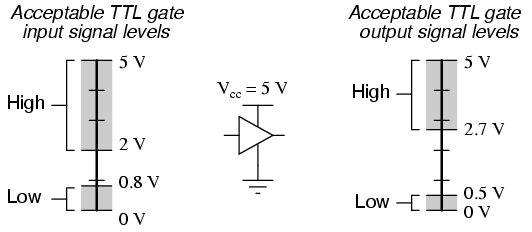
\includegraphics[scale=0.5]{logic_levels.png}
	\caption{TTL logic levels}
	\label{TTL_logic_levels}
\end{figure}

As shown in \autoref{TTL_logic_levels} we have some margin to make our PMOS and NMOS transistors work with each other in order to form a CMOS circuit which is actually working without getting warm.

Or more clearly defined
\begin{equation}
V_{off} \leq 0.8V
\end{equation}
and
\begin{equation}
V_{on} \geq 2V
\end{equation}
which are limits, elementary to our design.

\begin{figure}[H]
	\centering
	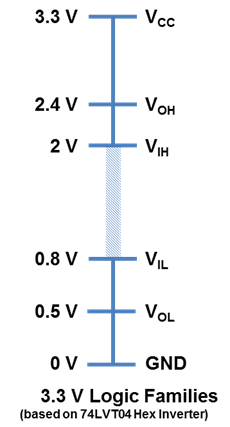
\includegraphics[scale=0.5]{cmos_3v3.png}
	\caption{CMOS 3.3V logic levels}
	\label{CMOS_logic_levels}
\end{figure}

This means that we also will be compatible to CMOS logic level output pins since their ON/OFF levels are within our tolerance range\footnote{\url{https://learn.sparkfun.com/tutorials/logic-levels/33-v-cmos-logic-levels}} as it is shown in \autoref{CMOS_logic_levels}.

We target threshold voltages of $V_{Tn} \approx 0.8V$ and $V_{Tp} \approx -0.8V$ which should be enough.
We can internally always shift the voltage supply levels to compensate for threshold variations.\footnote{Hagen! Please explain this part here}
\newpage
\input{process_design_requirements.tex}
\subsection{Substrate}
For this process p-substrate is being used, but forks and modifications will be very well possible based on a Graphene substrate or alike, still under the LSPL.
The starting material is a p-type, <100> oriented silicon with a doping concentration of $\approx 9\times10^{14}cm^{-3}$.\\

\textbf{Reasons for using p-substrate}:\begin{itemize}
\item We can't use two different substrates for our design because in the design both PMOS and NMOS is present.
We have to choose which is more beneficial from fabrication point of view.
In general or say it's true that NMOS devices are always more in the Semiconductor Industry in comparison to PMOS devices.
For your reference-SRAM requires 6 transistors (4 NMOS, 2 PMOS).
\item Another reason for more number of NMOS is because of difference of mobility of electron and holes.
Electron mobility is almost twice of holes mobility and because of this ON-RESISTANCE of n-channel device is half of p-channel device with the same geometry and under the same operating conditions.
That means to achieve same impedance size of n-channel transistors is almost half of p-channel devices.
Same thing I can say in the different way that for same size of wafer, we can have more number of NMOS (means can perform more logical operation) in comparison to PMOS.
\end{itemize}
\subsection{Isolation}
For the isolation (\autoref{sti})  in this design the STI approach is being chosen.
Shallow trench isolation (STI), also known as box isolation technique, is an integrated circuit feature which prevents electric current leakage between adjacent semiconductor device components.\footnote{\url{https://www.google.com/patents/US7985656}}
STI is generally used on CMOS process technology nodes of 250 nanometers and smaller.\\

\textbf{Reasons for using box isolation}:\begin{itemize}
\item We want to be forward compatible to future LibreSilicon nodes with a size of 100nm or smaller
\item It simplifies the construction of the gate and allows us to use Aluminum instead of Polysilicon for the gate contact
\end{itemize}

\subsection{Interconnect}
The interconnects and the gate electrode are being made using Aluminum which is a very commonly used material to do interconnects in low-frequency and low-resolution applications \\

\textbf{Reasons for using Aluminum}:\begin{itemize}
\item It's a well explored material for interconnect with a lot of literature on how to process it
\item Aluminum is easy to etch compared to copper
\item It isn't contaminating everything like copper does and doesn't require special separated setup for handling
\item The machines at HKUST can do CMP for copper only on 4 inch wafers which would limit us in wafer size
\end{itemize}

\begin{mdframed}[linewidth=2pt,linecolor=green]
As soon as we've got CMOS all figured out, we will tackle copper interconnect in release 2.0
\end{mdframed}
\newpage
\section{MOS gate material}
We decided to use the gate-first approach because realizing the gate self-alignment is much easier this way.
We further on decided to use the best-practice material polysilicon for the gate electrode, because it is easy to deposit and etch and virtually every manufacturer out there has at least one machine in their lab to deposit it.
Because of its high resistance however, we had to throw in another layer of silicide in order to reduce the gate resistivity from these $100 \Omega-m$ or so to a a few Ohms per meter.
A nice side effect is the better etch-stop properties of this low-resistance film adding to the gate, source and drain contacts.

A down side is that we will have to get "a hang on" the reaction times of silicides because a lot of the details of the reactivity between silicon and titanium to form titanium-silicide seem to be under NDA and secrets of the diverse factories running their own CMOS processes.

\section{MOS gate thickness}\label{gate_dimensioning}
As the continuous down-scaling of the device size has lead to very thin gate oxides, the leakage current that can flow from the channel to the gate comes into the order of the subthreshold leakage current and the gate cannot be considered as an ideally insulated electrode anymore.
This affects the circuit functionality and increases the standby power consumption due to the static gate current.
For dynamic logic concepts the gate leakage drastically reduces the maximum clock cycle time\footnote{N. Wang, Digital MOS Integrated Circuits, Prentice-Hall, Englewood Cliffs, NJ, 1989}.
Two tunneling mechanisms are responsible for the gate leakage, Fowler-Nordheim tunneling and direct tunneling\footnote{A. Schenk and G. Heiser, "Modeling and Simulation of Tunneling through Ultra-Thin Gate Dielectrics"J.Appl.Phys., vol. 81, no. 12, pp. 7900, 1997}.
The gate leakage increases exponentially as the oxide thickness is reduced.
This limits the down-scaling of the oxide thickness to about 1.5-2 nm when looking at the total standby power consumption of a chip\footnote{Y. Taur, "The Incredible Shrinking Transistor," IEEE Spectrum, pp. 25-29, July 1999.}.
To further decrease the effective oxide thickness alternative high dielectric constant materials can be used\footnote{S. Thompson, P. Packan, and M. Bohr, "MOS Scaling: Transistor Challenges for the 21st Century," Intel Technology Journal, vol. Q3, 1998}.
On the other hand, a thin gate oxide reduces the short-channel effect and improves the driving capabilities of a MOS transistor.
However, a tradeoff between this benefit and the gate leakage is necessary.\\

With $1 \mu m$ we don't have to worry about this leakage yet because our gate oxide thickness is too high for these effects to actually become a problem, but we want to do our home work already in preparation of scale-down and also for curiosity.

We for now just use 40 nm. That's still doable with a precision high enough when using dry oxidation and a temperature of 1000\degree Celsius.

\subsection{Subthreshold leakage}\label{sub_threshold_leakage}

The sub-threshold leakage current can be calculated with\footnote{\url{http://ecee.colorado.edu/\~bart/book/book/chapter3/ch3_4.htm\#3_4_2}}
\begin{equation}
I_{sub}
=
I_0
\cdot
\left(1-\exp\left(-\frac{V_{ds}}{V_{th}}\right)\right)
\cdot
\exp\left(\frac{V_{gs}-V_{T}}{n \cdot V_{th}}\right)
\end{equation}

where
\begin{equation}
I_0 = \frac{W}{L} \mu_0 V_{th}^2 \sqrt{\frac{N_A \cdot q \cdot \epsilon_{Si}}{2 \cdot \phi_{sub}}}
\end{equation}
$V_{th}=26mV$ is the thermal voltage, $V_T$ is the threshold voltage, $V_{ds}$ and $V_{gs}$ are the drain-to-source and gate-to-source voltages respectively.
W and L are the effective transistor width and length, respectively. $C_{ox}$ is the gate oxide capacitance, $\mu_0$ is the carrier mobility and $n=1+\frac{C_{dep}}{C_{ox}}$ is the subthreshold swing coefficient.

First of all, lets say $W=L$ which leads to a square:
\begin{equation}
I_0 = \mu_0 V_{th}^2 \sqrt{\frac{N_A \cdot q \cdot \epsilon_{Si}}{2 \cdot \phi_{sub}}}
\end{equation}

With
\begin{itemize}
\item $\epsilon_0 = 8.85 \cdot 10^{-14}\frac{F}{cm}. $ is the electric permittivity in vacuum
\item $\epsilon_{ox} =3.9 \cdot \epsilon_0$ is the relative permittivity of silicon dioxide
\item $\epsilon_{Si} =11.68 \cdot \epsilon_0$ is the relative permittivity of silicon
\end{itemize}

The carrier mobility $ \mu_0$ can be calculated with\footnote{\url{https://ecee.colorado.edu/\~bart/book/book/chapter2/ch2_7.htm\#2_7_2}}
\begin{equation}
 \mu(N) =  \mu_{min} + \frac{ \mu_{max}- \mu_{min}}{1+\left(\frac{N}{N_r}\right)^\alpha}
\end{equation}
using the fitting parameters from \autoref{fitting_parameters_mobility}

\begin{table}[H]
	\centering
	\begin{tabular}{|c|c|c|c|}
		\hline
		{} &
		\textbf{Arsenic} &	
		\textbf{Phosphorus} &
		\textbf{Boron} \\
		\hline
		$\mu_{min} [\frac{cm^2}{Vs}]$ &
		52.2 &
		68.5 &		
		44.9 \\
		\hline
		$\mu_{max} [\frac{cm^2}{Vs}]$ &
		1417 &
		1414 &
		470.5 \\
		\hline
		$N_r [\frac{1}{cm^3}]$ &
		$9.68 \cdot 10^{16}$ &
		$9.20 \cdot 10^{16}$ &
		$2.23 \cdot 10^{17}$ \\
		\hline
		$\alpha$ &
		0.68 &
		0.711 &
		0.719 \\
		\hline
	\end{tabular}
	\caption{Parameters for calculation of the mobility as a function of the doping density}
	\label{fitting_parameters_mobility}
\end{table}

\subsection{Gate tunneling current}

The tunneling of electrons (or holes) from the bulk and source/drain overlap region through the gate oxide potential barrier into the gate (or vice-versa) is referred as gate oxide tunneling current.
This phenomenon is related with the MOS capacitance concept.
There are three major gate leakage mechanisms in a MOS structure.
The first one is the electron conduction-band tunneling (ECB), where electrons tunneling from conduction band of the substrate to the conduction band of the gate (or vice versa).
The second one is the electron valence-band tunneling (EVB). In this case, electrons tunneling from the valence band of the substrate to the conduct band of the gate.
The last one is known as hole valence-band (HVB) tunneling, where holes tunneling from the valence band of the substrate to the valence band of the gate (or vice- versa)

Each mechanism is dominant or important in different regions of operation for NMOS and PMOS transistors. For each mechanism, gate leakage current can be modeled by
\begin{equation}
I = W \cdot L \cdot A \cdot \left(\frac{V_{ox}}{t_{ox}}\right)^2\exp\left(\frac{-B\left(1-\left(1-\frac{V_{ox}}{\phi_{ox}}\right)^{\frac{3}{2}}\right)}{\frac{T_{ox}}{t_{ox}}}\right)
\end{equation}

\newpage
\subsection{NMOS threshold}\label{nmos_dimensioning}
First we take a look at the worst case of 4 stacked NMOS transistors, which is the highest stacking amount which will be possible in technologies relying on this process.

%%  ************    LibreSilicon's StdCellLibrary   *******************
%%
%%  Organisation:   Chipforge
%%                  Germany / European Union
%%
%%  Profile:        Chipforge focus on fine System-on-Chip Cores in
%%                  Verilog HDL Code which are easy understandable and
%%                  adjustable. For further information see
%%                          www.chipforge.org
%%                  there are projects from small cores up to PCBs, too.
%%
%%  File:           StdCellLib/Documents/LaTeX/schematic_AND4.tex
%%
%%  Purpose:        Schematic File for AND4
%%
%%  ************    LaTeX with circdia.sty package      ***************
%%
%%  ///////////////////////////////////////////////////////////////////
%%
%%  Copyright (c) 2018 by chipforge <hsank@nospam.chipforge.org>
%%  All rights reserved.
%%
%%      This Standard Cell Library is licensed under the Libre Silicon
%%      public license; you can redistribute it and/or modify it under
%%      the terms of the Libre Silicon public license as published by
%%      the Libre Silicon alliance, either version 1 of the License, or
%%      (at your option) any later version.
%%
%%      This design is distributed in the hope that it will be useful,
%%      but WITHOUT ANY WARRANTY; without even the implied warranty of
%%      MERCHANTABILITY or FITNESS FOR A PARTICULAR PURPOSE.
%%      See the Libre Silicon Public License for more details.
%%
%%  ///////////////////////////////////////////////////////////////////
    \begin{figure}[H]
	\centering
            \begin{circuitdiagram}{50}{33}
            \pin{2}{2.5}{L}{A}  % pin A, n-channel below
            \pin{2}{8.5}{L}{B}  % pin B, n-channel middle
            \pin{2}{14.5}{L}{C} % pin C, n-channel middle
            \pin{2}{20.5}{L}{D} % pin D, n-channel above
            \pin{2}{29.5}{L}{A} % pin A, p-channel left
            \pin{14}{29.5}{L}{B} % pin B, p-channel middle
            \pin{26}{29.5}{L}{C} % pin C, p-channel middle
            \pin{38}{29.5}{L}{D} % pin D, p-channel right
            \trans{nenh*}{6}{4}{R}{}{}  % nmos below
            \trans{nenh*}{6}{10}{R}{}{} % nmos middle
            \trans{nenh*}{6}{16}{R}{}{} % nmos middle
            \trans{nenh*}{6}{22}{R}{}{} % nmos above
            \trans{nenh*}{54}{22}{R}{}{} % nmos inverter
            \trans{penh*}{6}{28}{R}{}{} % pmos left
            \trans{penh*}{18}{28}{R}{}{} % pmos middle
            \trans{penh*}{30}{28}{R}{}{} % pmos middle
            \trans{penh*}{42}{28}{R}{}{} % pmos right
            \trans{penh*}{54}{28}{R}{}{} % pmos inverter
            \wire{8}{6}{8}{8}     % wire between nmos
            \ground{8}{0.5}{D}  % ground below nmos
            \ground{56}{18.5}{D}  % ground below inverter
            \power{8}{31.5}{U}{}  % power above left pmos
            \power{20}{31.5}{U}{}  % power above middle pmos
            \power{32}{31.5}{U}{}  % power above middle pmos
            \power{44}{31.5}{U}{}  % power above right pmos
            \power{56}{31.5}{U}{}  % power above inverter
            \wire{8}{12}{8}{14}     % wire between nmos
            \wire{8}{18}{8}{20}     % wire between nmos and pmos
            \wire{20}{25}{20}{26}
            \wire{32}{25}{32}{26}
            \wire{44}{25}{44}{26}
            \wire{8}{25}{51}{25}    % wire before inverter gate
            \junct{8}{25}
            \junct{20}{25}
            \junct{32}{25}
            \junct{44}{25}
            \junct{56}{25}
            \wire{51}{29.5}{51}{20.5}   % wire at inverter gates
            \junct{51}{25}
            \wire{56}{25}{58}{25}    % wire before pin Z
            \pin{59}{25}{R}{Z}  % pin Z
            \end{circuitdiagram}
            \caption{AND4 gate}
    \end{figure}
As shown in  \autoref{TTL_logic_levels} our acceptable voltages for our CMOS "ON" state range from 2V to VDD (which typically is around $5V\pm0.25V$)

\begin{equation}
V_{on} \geq 2V
\end{equation}

Because there are four transistors dividing the voltage by being in series, the power supply voltage is being divided by the amount of transistors in series.
In order to match the threshold voltages of all of the transistors, which is needed for a working digital logic, the following equation need to be satisfied

\begin{equation}
V_{on} > 4 \cdot V_{Tn}
\end{equation}

Lets assume the worst case with

\begin{equation}
V_{on} = 2V
\end{equation}

Which leads to the required worst case threshold tolerance value

\begin{equation}
4 \cdot V_{Tn} < 2V
\Rightarrow
V_{Tn} < 500mV
\end{equation}
 
With the values derived from \autoref{gate_dimensioning} and a surface concentration for our P-well of $10^{22}\frac{1}{m^3}$ we are already set because $\approx 0.39V$ are already better than we need.

We target a concentration of $N_p = 10^{16}\frac{1}{cm^3}=10^{22}\frac{1}{m^3}$.

The depletion zone thickness at its peak will be $W_{dmax} \approx 2.73 \cdot 10^{-7} m = 273 nm$

With an implantation (or constant source diffusion step), we can now set a range/energy and dosage in order to cover the depletion zone area.

For getting the energy and dose we look at \autoref{graphics_range_and_straggle} or use the web tool linked in the implant chapter.

The depth of the p-well $\approx 2 \mu m$ comes mainly from the need to fulfill the condition from \autoref{physics_drive_in}

\begin{equation}
x_e = 2 \cdot \sqrt{D_e \cdot t_e} \gg 2 \cdot \sqrt{D_v \cdot t_v} = x_v
\end{equation}

\newpage

We already got the background ($N_B \approx 7 \cdot 10^{14} \frac{1}{cm^3}=7 \cdot 10^{20} \frac{1}{m^3}$) concentration from the specs of the basis substrate.

\begin{equation}
N_p - N_B = 10^{22}\frac{1}{m^3} - 7 \cdot 10^{20} \frac{1}{m^3} = 9.3 \cdot 10^{21} \frac{1}{m^3}
\end{equation}

We use a drive in temperature of $1150 \degree C$ which is  $T = 1423.15 \degree K$ in Kelvin which gives us the diffusion coefficient $D=9.1 \cdot 10^{-17}  \frac{m^2}{s}$

Now using
\begin{equation}
N(x,t)
=
\frac{Q}{\sqrt{\pi\cdot D \cdot t}} \cdot \exp\left(\frac{-x^2}{4 \cdot D \cdot t}\right)
\end{equation}

We set the conditions and get the required diffusion time as well as the initial dosage in one shot:
\begin{equation}
N(0,t)
=
\frac{Q}{\sqrt{\pi\cdot D \cdot t}}
=
N_p-N_B
=
7 \cdot 10^{20} \frac{1}{m^3}
\end{equation}
\begin{equation}
x
=
2 \cdot \sqrt{D \cdot t}
=
2 \mu m
=
2 \cdot 10^{-6} m
\end{equation}
\begin{equation}
\Rightarrow
t \approx 11018s \approx \underline{3h}
\end{equation}
\begin{equation}
\Rightarrow
Q
=
7 \cdot 10^{20} \frac{1}{m^3} \cdot \sqrt{\pi\cdot D \cdot t}
\approx
\underline{1.64 \cdot 10^{16} \frac{1}{m^2}}
\end{equation}

If we plot the functions from our calculation we can yield the below graphics\footnote{see simulation/diffusion\_pwell.wxmx}

\begin{figure}[H]
	\centering
	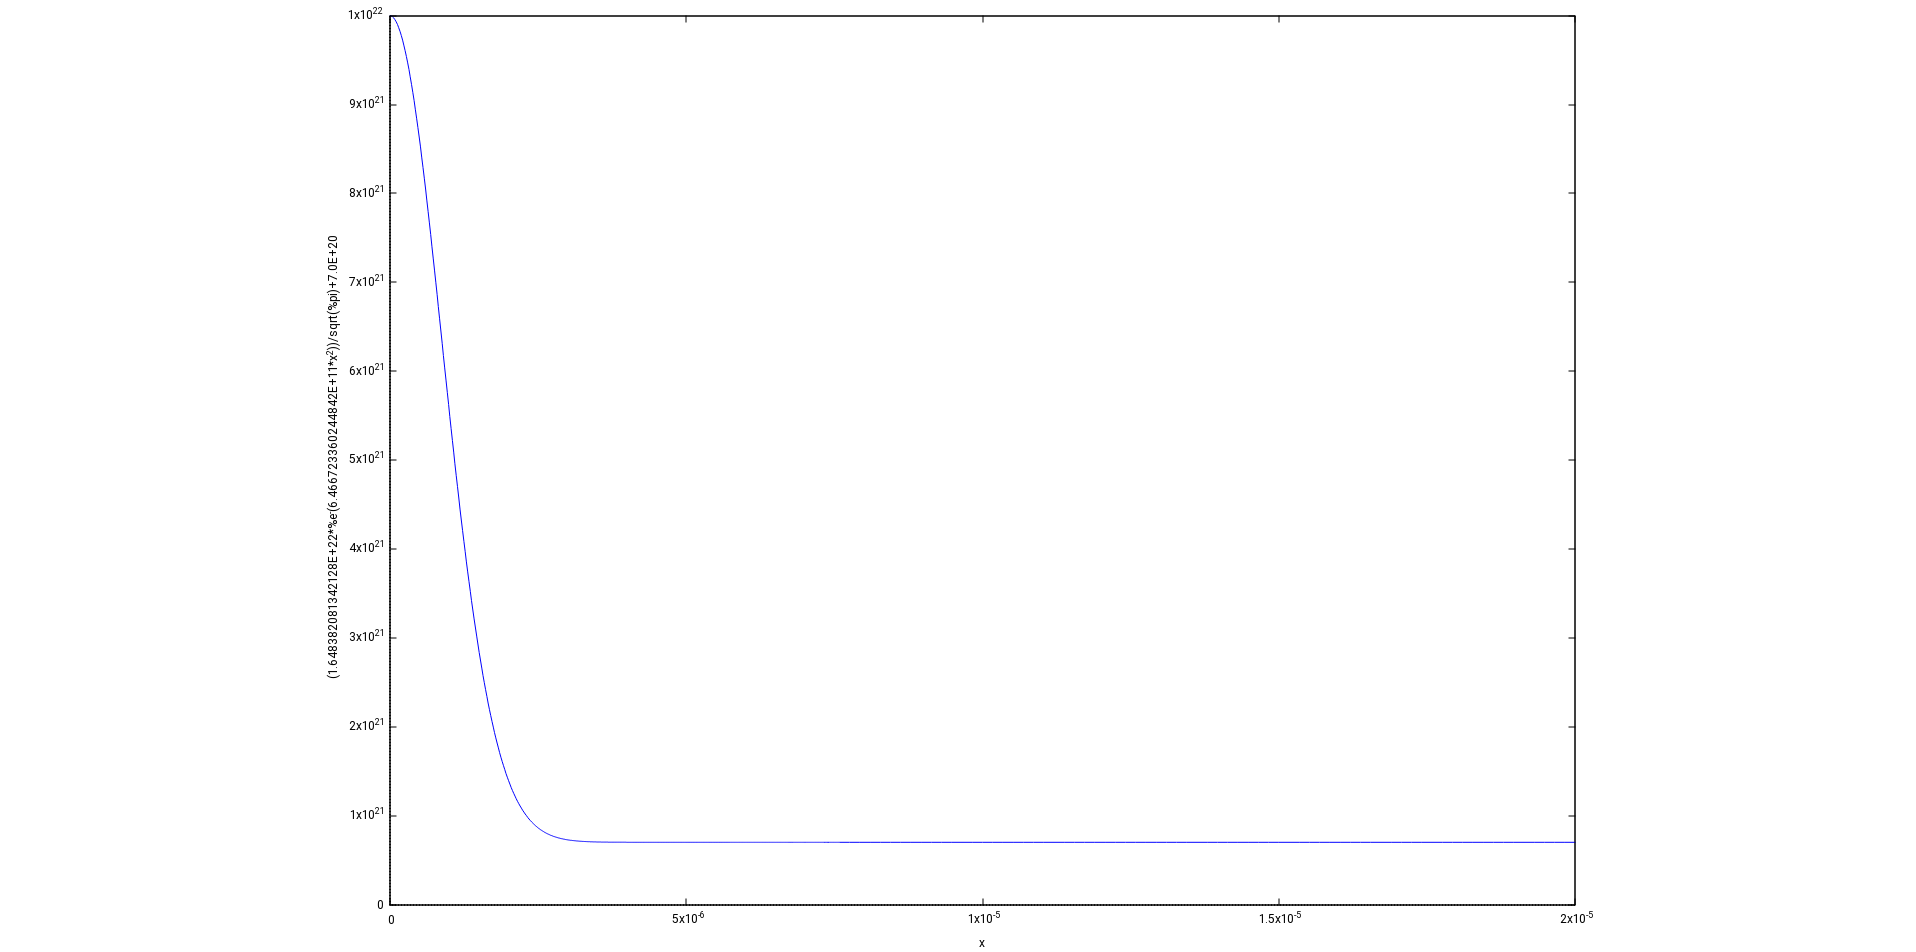
\includegraphics[width=0.75\textwidth]{p-well-diffusion.png}
	\caption{Dopant concentration after 3 hours}
	\label{pwell_drive_in_outcome}
\end{figure}

In \autoref{pwell_drive_in_outcome} we can see that after three hours we already have the desired even gradient which and deep penetration of dopants, which will give us a low $R_{DS}$.
\newpage
\subsection{PMOS threshold}
Now we take a look at the worst case of 4 stacked PMOS transistors, which is the highest stacking amount which will be possible in technologies relying on this process.
%%  ************    LibreSilicon's StdCellLibrary   *******************
%%
%%  Organisation:   Chipforge
%%                  Germany / European Union
%%
%%  Profile:        Chipforge focus on fine System-on-Chip Cores in
%%                  Verilog HDL Code which are easy understandable and
%%                  adjustable. For further information see
%%                          www.chipforge.org
%%                  there are projects from small cores up to PCBs, too.
%%
%%  File:           StdCellLib/Documents/LaTeX/schematic_OR4.tex
%%
%%  Purpose:        Schematic File for OR4
%%
%%  ************    LaTeX with circdia.sty package      ***************
%%
%%  ///////////////////////////////////////////////////////////////////
%%
%%  Copyright (c) 2018 by chipforge <hsank@nospam.chipforge.org>
%%  All rights reserved.
%%
%%      This Standard Cell Library is licensed under the Libre Silicon
%%      public license; you can redistribute it and/or modify it under
%%      the terms of the Libre Silicon public license as published by
%%      the Libre Silicon alliance, either version 1 of the License, or
%%      (at your option) any later version.
%%
%%      This design is distributed in the hope that it will be useful,
%%      but WITHOUT ANY WARRANTY; without even the implied warranty of
%%      MERCHANTABILITY or FITNESS FOR A PARTICULAR PURPOSE.
%%      See the Libre Silicon Public License for more details.
%%
%%  ///////////////////////////////////////////////////////////////////
    
    \begin{figure}[H] %\caption{Schematic}
       \centering
            \begin{circuitdiagram}{60}{33}
            \pin{2}{2.5}{L}{A}  % pin A, n-channel left
            \pin{2}{11.5}{L}{A}  % pin A, p-channel below
            \pin{2}{17.5}{L}{B}  % pin B, p-channel middle
            \pin{2}{23.5}{L}{C} % pin C, p-channel above
            \pin{2}{29.5}{L}{D} % pin D, p-channel above
            \pin{14}{2.5}{L}{B} % pin B, n-channel middle
            \pin{26}{2.5}{L}{C} % pin C, n-channel right
            \pin{38}{2.5}{L}{D} % pin D, n-channel right
            \trans{nenh*}{6}{4}{R}{}{}  % nmos left
            \trans{penh*}{6}{10}{R}{}{} % pmos below
            \trans{penh*}{6}{16}{R}{}{} % pmos middle
            \trans{penh*}{6}{22}{R}{}{} % pmos above
            \trans{penh*}{6}{28}{R}{}{} % pmos above
            \trans{nenh*}{18}{4}{R}{}{} % nmos middle
            \trans{nenh*}{30}{4}{R}{}{} % nmos right
            \trans{nenh*}{42}{4}{R}{}{} % nmos right
            \wire{8}{6}{8}{8}     % wire between nmos
            \ground{8}{0.5}{D}  % ground below nmos
            \power{8}{31.5}{U}{}  % power above left pmos
            \ground{20}{0.5}{D}  % ground below nmos
            \ground{32}{0.5}{D}  % ground below nmos
            \ground{44}{0.5}{D}  % ground below nmos
            \wire{8}{12}{8}{14}     % wire between nmos
            \wire{8}{18}{8}{20}     % wire between nmos and pmos
            \wire{20}{7}{20}{6}
            \wire{32}{7}{32}{6}
            \wire{8}{7}{51}{7}    % wire before inverter gates
            \wire{51}{2.5}{51}{11.5}  % wire on inverter gates
            \junct{8}{7}
            \junct{20}{7}
            \junct{32}{7}
            \junct{44}{7}
            \junct{51}{7}
            \trans{nenh*}{54}{4}{R}{}{} % nmos right
            \trans{penh*}{54}{10}{R}{}{} % pmos below
            \power{56}{13.5}{U}{}  % power above left pmos
            \ground{56}{0.5}{D}  % ground below nmos
            \wire{56}{7}{58}{7}    % wire before pin
            \wire{56}{6}{56}{8}    % wire before pin
            \junct{56}{7}
            \pin{59}{7}{R}{Z}  % pin Z
            \end{circuitdiagram}
            \caption{OR4 gate}
    \end{figure}

\newpage
\subsection{MOS gate verification}\label{gate_verify}
Now we have to verify that we don have relevant leakage on the gate with the thresholds and doping values we've set.

For that we use the formulas from \autoref{sub_threshold_leakage}

We can now plot multiple leakages for N- and P-channel transistors with a gate oxide thickness\footnote{See simulation/gate.wxmx} and with a surface concentration of $1e16\frac{1}{cm^3}=1e22\frac{1}{m^3}$ each
\begin{figure}[H]
	\centering
	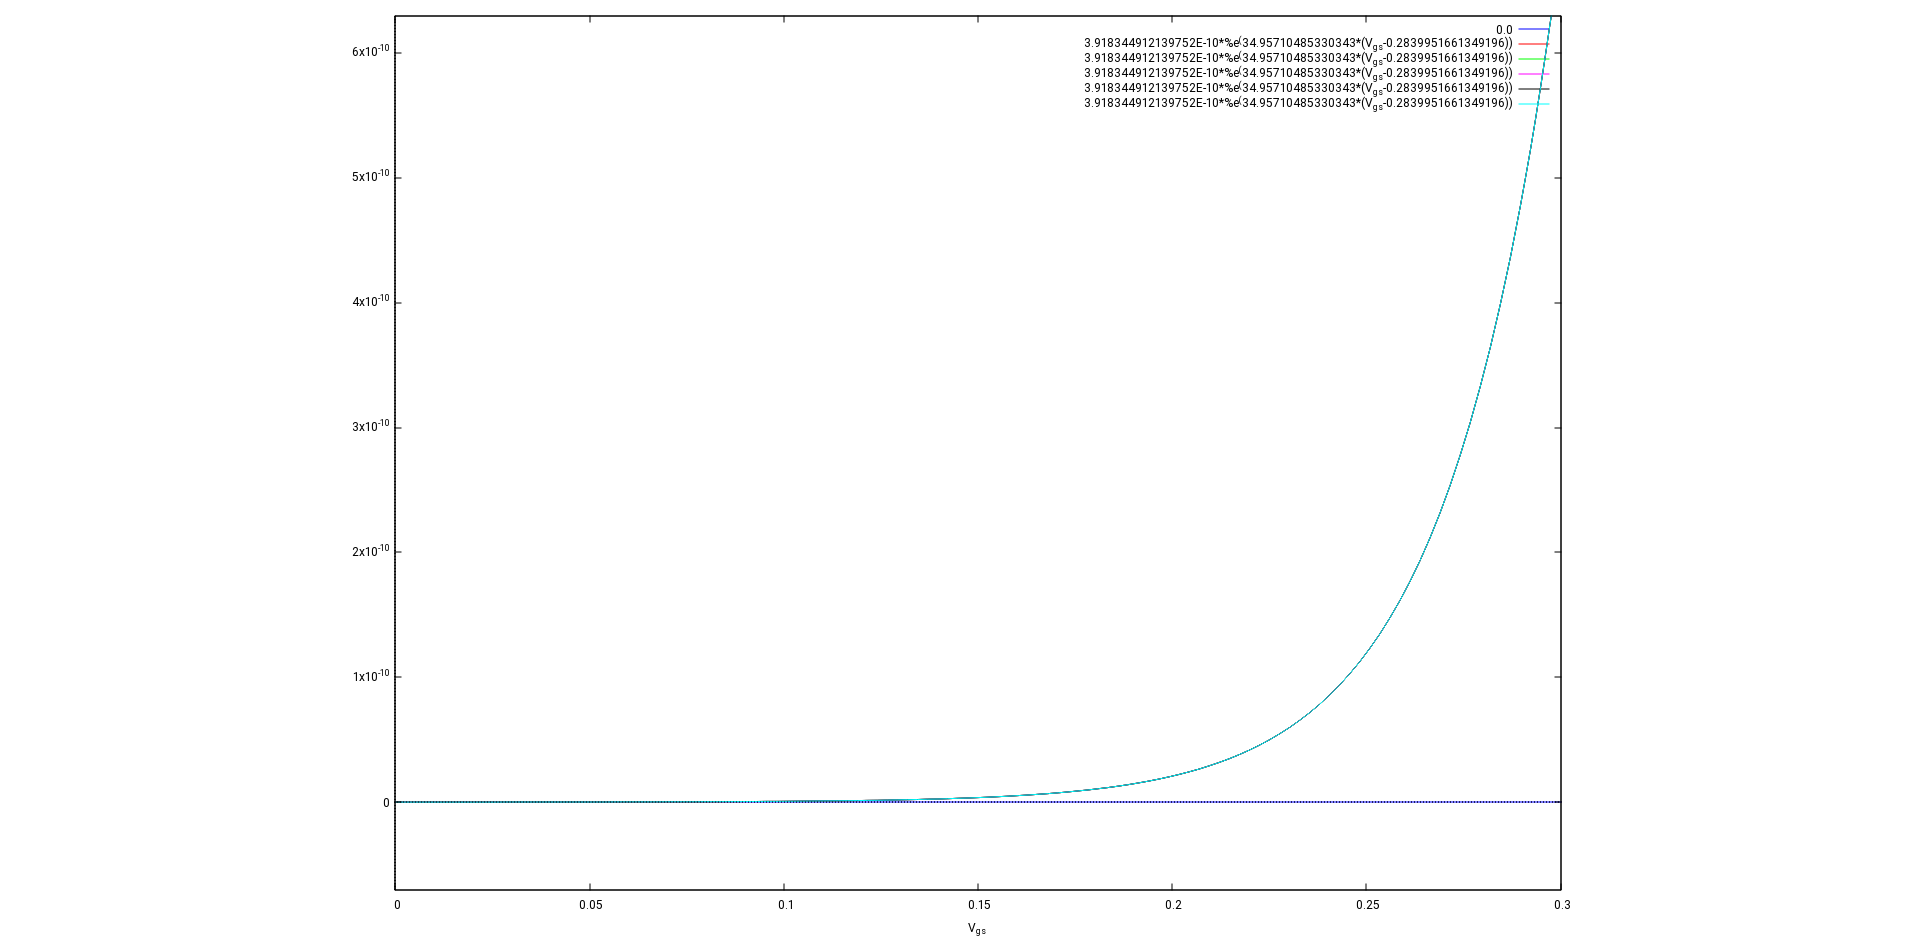
\includegraphics[width=\textwidth]{subthreshold_leagage.png}
	\caption{Subthreshold leakage plot(in Ampere)}
	\label{leagage_currents}
\end{figure}
In \autoref{leagage_currents} we see that with our gate oxide thickness this is really no problem, as we had expected.
From 0V up to 5V and further there is basically no leakage on the gate from the sub threshold current with $V_{Tn} \approx 0.39V$ and $V_{Tp} \approx -0.30V$.
That's good enough, as we will see in \autoref{nmos_dimensioning} and \autoref{pmos_dimensioning}.
There is actually a reduction of current when reaching the threshold because of the inversion of the capacity in the depletion zone\footnote{\url{https://people.eecs.berkeley.edu/~hu/Chenming-Hu_ch5.pdf}}, but I didn't include this into the calculation, because "TL;DR".
It's a TODO for release 2.1 of this process which will go sub $1 \mu m$
\newpage
\newcommand{\addAlignmentCross}[2]{
	\draw[line width=1.5mm, active,opacity=\OpacityLayout] (#1,#2+0.5) -- (#1+1,#2+0.5);
	\draw[line width=1.5mm, active,opacity=\OpacityLayout] (#1+0.5,#2) -- (#1+0.5,#2+1);
}

\section{Alignment strategy}
When having multiple layers exposed after each other, there is the problem on how to make sure that for instance vias are actually making contact with the below wire and the wire above.
For this purpose we have to align the masks, in order to avoid issues like shown in \autoref{what_can_go_wrong_with_alignment}

\begin{figure}[H]
	\centering
	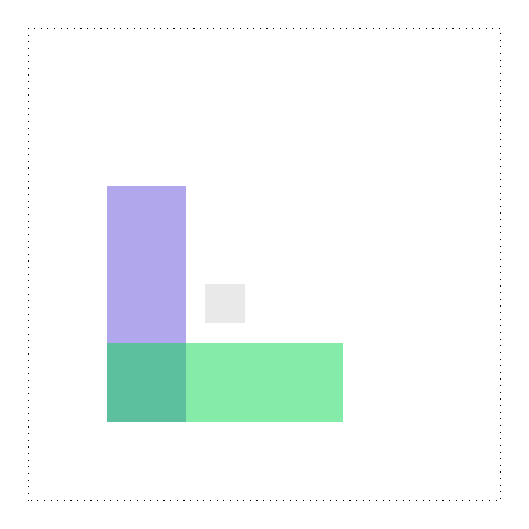
\begin{tikzpicture}
		\fill[metal1,opacity=\OpacityLayout] (1,1) rectangle (2,4);
		\fill[via1,opacity=\OpacityLayout] (2.25,2.25) rectangle (2.75,2.75);
		\fill[metal2,opacity=\OpacityLayout] (1,1) rectangle (4,2);
		\draw[dotted] (0.0,0) rectangle (6,6);
	\end{tikzpicture} 
	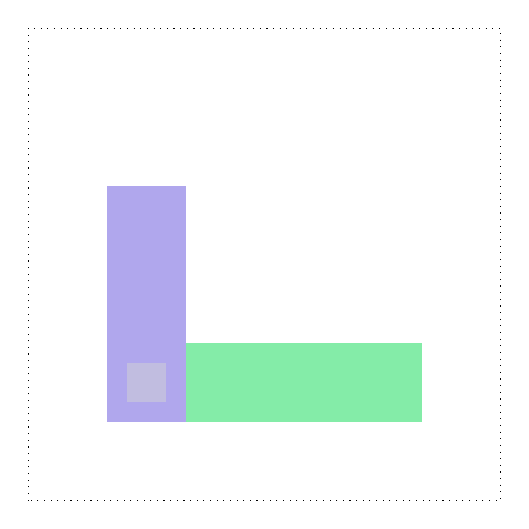
\begin{tikzpicture}
		\fill[metal1,opacity=\OpacityLayout] (1,1) rectangle (2,4);
		\fill[via1,opacity=\OpacityLayout] (1.25,1.25) rectangle (1.75,1.75);
		\fill[metal2,opacity=\OpacityLayout] (2,1) rectangle (5,2);
		\draw[dotted] (0.0,0) rectangle (6,6);
	\end{tikzpicture}
	\caption{What can go wrong with alignment}
	\label{what_can_go_wrong_with_alignment}
\end{figure}

In \autoref{what_can_go_wrong_with_alignment} we can see how the wires and vias are missing each other because of an exposure offset and the via is going nowhere in the best case and creates an (of course) undesired short circuit in the worst case. This has to be avoided by using alignment.

We have decided to use backside alignment because shining through the wafer from behind with infrared and finding an orientation marker isn't a problem with our simple CMOS process.\footnote{\url{https://patents.google.com/patent/US6376329}}

The stepper machine at HKUST\footnote{\url{http://www.nff.ust.hk/en/equipment-and-process/equipment-list/photolithography-module.html}} does that for us.

We need to add orientation cross hairs onto the layout edge in order to identify them during alignment

\begin{figure}[H]
	\centering
	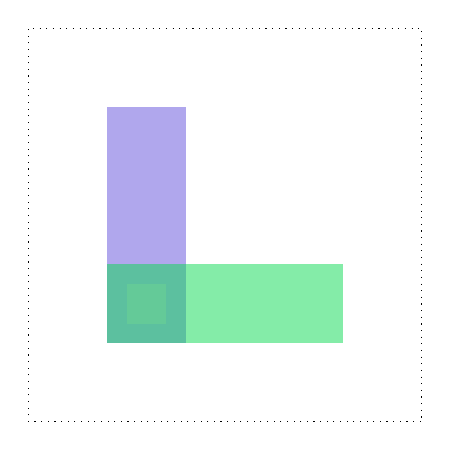
\begin{tikzpicture}
		\fill[metal1,opacity=\OpacityLayout] (1,1) rectangle (2,4);
		\fill[via1,opacity=\OpacityLayout] (1.25,1.25) rectangle (1.75,1.75);
		\fill[metal2,opacity=\OpacityLayout] (1,1) rectangle (4,2);
		\draw[dotted] (0.0,0) rectangle (5,5);
		% cross one
		\addAlignmentCross{0}{0}
		% cross two
		\addAlignmentCross{4}{4}
		% cross three
		\addAlignmentCross{4}{0}
		% cross four
		\addAlignmentCross{0}{4}
	\end{tikzpicture}
	\caption{Mask alignment with markers}
\end{figure}

Using the STI (active) mask for the cross hair structure is a good choice, because it's the lowest layer, will never be covered by any additional material and gives us a good contrast because it's silicon next to silicon dioxide.

\newpage

The "DRIE Etcher" can't etch more precise than $0.5 \mu m$ (Minimum Line/Space: $0.5 \mu m$) which means we will have to give the cross hair structure with the dimensions as shown in \autoref{cross_hair_dimensions}
\begin{figure}[H]
	\centering
	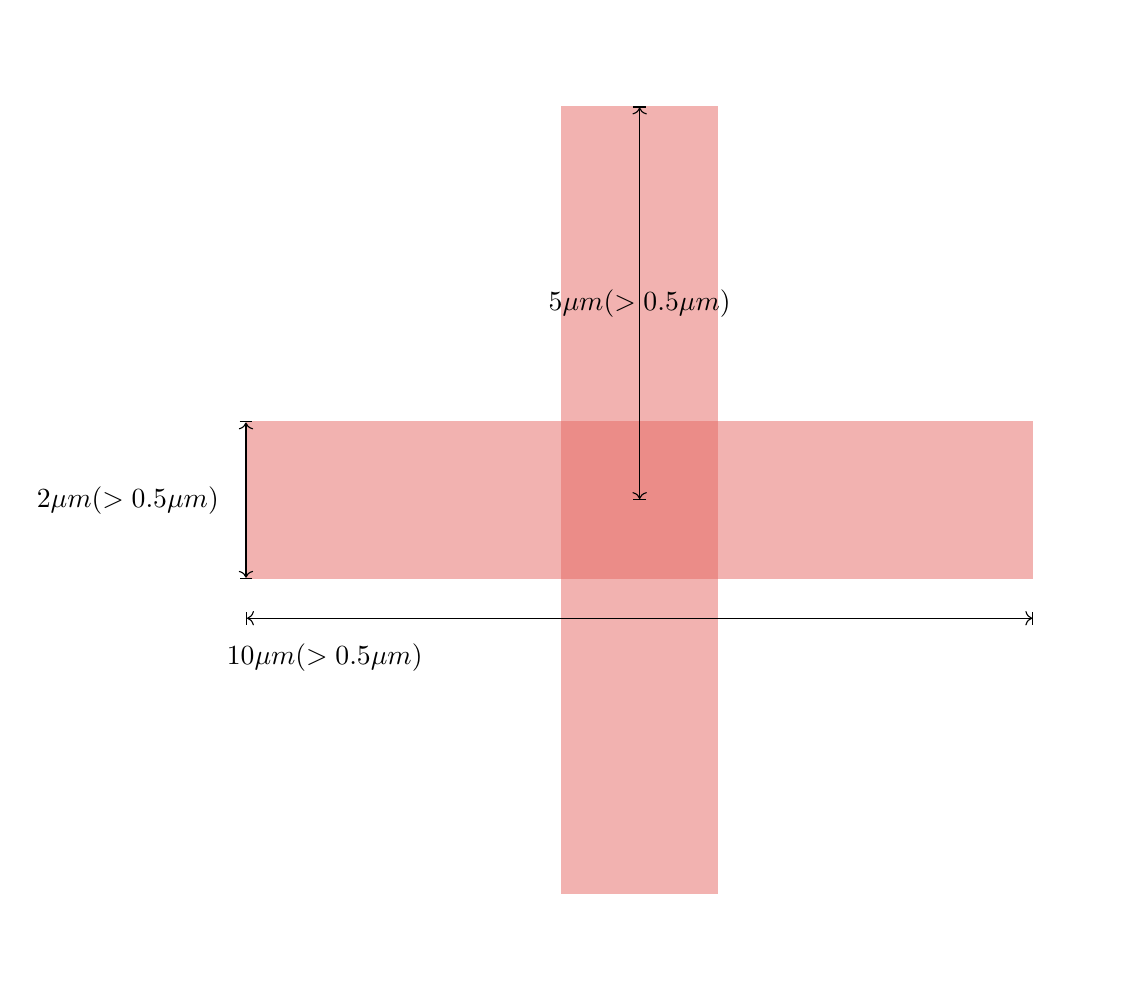
\begin{tikzpicture}
		\draw[line width=20mm, active,opacity=\OpacityLayout] (0,50mm) -- (100mm,50mm);
		\draw[line width=20mm, active,opacity=\OpacityLayout] (50mm,0) -- (50mm,100mm);
		\draw [|<->|] (0,4) -- (0,6); 
		\node at (-15mm,50mm) {$ 2 \mu m (> 0.5 \mu m) $};
		\draw [|<->|] (0,3.5) -- (10,3.5); 
		\node at (10mm,30mm) {$ 10 \mu m (> 0.5 \mu m) $};
		\draw [|<->|] (50mm,50mm) -- (50mm,100mm); 
		\node at (50mm,75mm) {$ 5 \mu m (> 0.5 \mu m) $};
	\end{tikzpicture}
	\caption{Cross hair dimension}
	\label{cross_hair_dimensions}
\end{figure}

We can now manufacture masks as shown in \autoref{mask_set_example} and align them using the infrared light from the stepper mask alignment and the provided electronic microscope.

\begin{figure}[H]
	\centering
	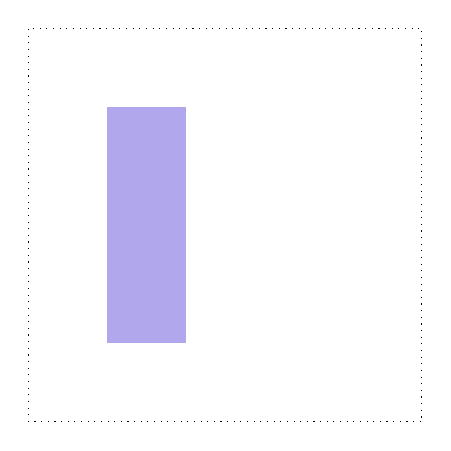
\begin{tikzpicture}
		\fill[metal1,opacity=\OpacityLayout] (1,1) rectangle (2,4);
		\draw[dotted] (0.0,0) rectangle (5,5);
		% cross one
		\addAlignmentCross{0}{0}
		% cross two
		\addAlignmentCross{4}{4}
		% cross three
		\addAlignmentCross{4}{0}
		% cross four
		\addAlignmentCross{0}{4}
	\end{tikzpicture} 
	\begin{tikzpicture}
		\fill[via1,opacity=\OpacityLayout] (1.25,1.25) rectangle (1.75,1.75);
		\draw[dotted] (0.0,0) rectangle (5,5);
		% cross one
		\addAlignmentCross{0}{0}
		% cross two
		\addAlignmentCross{4}{4}
		% cross three
		\addAlignmentCross{4}{0}
		% cross four
		\addAlignmentCross{0}{4}
	\end{tikzpicture} 
	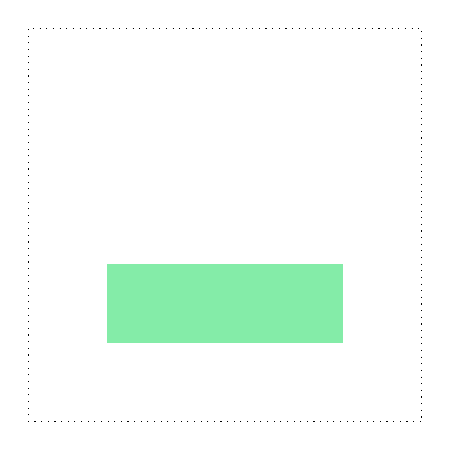
\begin{tikzpicture}
		\fill[metal2,opacity=\OpacityLayout] (1,1) rectangle (4,2);
		\draw[dotted] (0.0,0) rectangle (5,5);
		% cross one
		\addAlignmentCross{0}{0}
		% cross two
		\addAlignmentCross{4}{4}
		% cross three
		\addAlignmentCross{4}{0}
		% cross four
		\addAlignmentCross{0}{4}
	\end{tikzpicture}
	\caption{Layout masks with alignment markers}
	\label{mask_set_example}
\end{figure}
\newpage
\section{Simulation with parameters}
\newpage
\section{Process steps}
\tikzstyle{block} = [rectangle, draw, fill=blue!20, text width=3cm, text centered, rounded corners, minimum height=1.5cm]
\tikzstyle{line} = [draw, very thick, color=black!50, -latex']

The general flow chart of the overall process flow can be seen in \autoref{full_flow}.
These process steps will be discussed within the following sections.
\begin{figure}[H]
	\centering
	\begin{tikzpicture}[node distance=2cm, thick,scale=0.8, every node/.style={transform shape}]
		%% Place nodes
		%active CMOS				
		\node [block] (isolation) at (4,20) {Isolation (STI)\\ \autoref{sti}};
		\node [block, below of=isolation] (nwell) {N-Well\\ \autoref{nwell_chapter}};
		\node [block, below of=nwell] (pwell) {P-Well\\ \autoref{pwell_chapter}};
		\node [block, below of=pwell] (gate) {Gate\\ \autoref{gate}};
		\node [block, below of=gate] (np) {n+ Implant\\ \autoref{nimplant}};
		\node [block, below of=np] (pp) {p+ Implant\\ \autoref{pimplant}};
		\node [block, below of=pp] (silicification) {Silicification\\ \autoref{step_silicification}};
		%post proces
		\node [block] (via1) at (8,8) {First vias\\ \autoref{via1}};
		\node [block, above of=via1] (metal1) {First metal\\ \autoref{metal1}};
		\node [block, above of=metal1] (via2) {Additional vias\\ \autoref{via2}};
		\node [block, above of=via2] (metal2) {Additional metal\\ \autoref{metal2}};
		\node (repeat) at (10.5,14.5) {Repeat};

		%% Draw edges
		\path [line] (isolation) -- (nwell);
		\path [line] (nwell) -- (pwell);
		\path [line] (pwell) -- (gate);
		\path [line] (gate) -- (np);
		\path [line] (np) -- (pp);
		\path [line] (pp) -- (silicification);
		\path [line] (silicification) -- (via1);
		\path [line] (via1) -- (metal1);
		\path [line] (metal1) -- (via2);
		\path [line] (via2) -- (metal2);
		\path [line] (metal2) -- +(3,0) -- +(3,-2) -- (via2);

		\draw[dotted] (2,6) rectangle (6,21);
		\node at (4,6.5) {CMOS process};
		\draw[dotted] (6,6) rectangle (12,21);
		\node at (8,6.5) {Interconnect};

		%\draw[dotted] (1.5,9) rectangle (10.5,21.5);
		%\node at (4,9.5) {Front-end processing};

		%\draw[dotted] (11,9) rectangle (15,21.5);
		%\node at (13,9.5) {Back-end processing};
	\end{tikzpicture}
	\caption{Frontend and backend process flow}
	\label{full_flow}
\end{figure}
The six overall process steps are part of an active part of the technology, while the final metal (respectively contact) layers will be used for making a contact between the logic gates and macro cells and making them available to the exterior world.

For this process p-substrate is the required basic substrate, but forks and modifications will be very well possible based on a Graphene substrate or alike, still under the LSPL.
The starting material is a p-type, <100> oriented silicon with a doping concentration of $\approx 9\times10^{14}cm^{-3}$.\\



\label{process_overview}
\newpage
\section{Shallow trench isolation}\label{sti_chapter}
The geometry of a substrate with STI implemented can be seen in \autoref{sti_target}.

\begin{figure}[H]
	\centering
	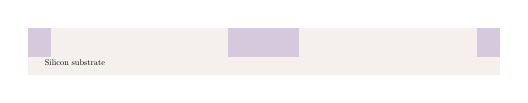
\begin{tikzpicture}[node distance = 3cm, auto, thick,scale=\CrossAndTopSectionBig, every node/.style={transform shape}]
		% substrate
\fill[substrate] (0,0) rectangle (20,2);
\node at (2,0.5) {Silicon substrate};
%trenches
\fill[isolationoxide] (0,0.75) rectangle (1,2);
\fill[isolationoxide] (8.5,0.75) rectangle (11.5,2);
\fill[isolationoxide] (19,0.75) rectangle (20,2);
	\end{tikzpicture}
	
\begin{tikzpicture}[node distance = 3cm, auto, thick,scale=\CrossAndTopSectionBig, every node/.style={transform shape}]
		% substrate
\fill[YellowOrange] (0,0) rectangle (20,12);
% trench area
\fill[DarkGray] (0,0) rectangle (1,12);
\fill[DarkGray] (8.5,0) rectangle (11.5,12);
\fill[DarkGray] (19,0) rectangle (20,12);
\fill[DarkGray] (0,0) rectangle (20,1.25);
\fill[DarkGray] (0,7.5) rectangle (20,12);
	\end{tikzpicture}
	\caption{Shallow trench isolation target geometry}
	\label{sti_target}
\end{figure}

As can be seen in \autoref{nwell_target}, the n-well and the STI trench are supposed to have approximately the same depth but the n-well and p-well go down a little bit further.
Because the n-well will be $\approx 4 \mu m$ in depth we have to match this with our trench depth.
I order to allow a sufficiently low resistance of the ESD diode but at the same time a sufficient isolation of between the standard cells a trade-ff has been done.
The targeted depth of the box isolation is $\approx 2 \mu m$.

\begin{figure}[H]
	\centering
	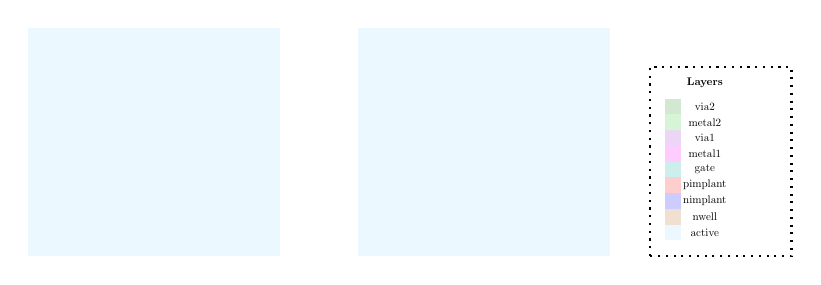
\begin{tikzpicture}[node distance =1cm, auto, thick,scale=\VLSILayout, every node/.style={transform shape}]
		\fill[nwell,opacity=0.2] (0.75,0.5) rectangle (8.75,7.75);
\fill[nwell,opacity=0.2] (11.25,0.5) rectangle (19.25,7.75);

\draw[dotted] (20.5,0.5) rectangle (25,6.5);

\node at (22.25,6) {\textbf{Layers}};

\fill[nwell,opacity=0.2] (21,1) rectangle (21.5,1.5);
\node at (22.25,1.25) {active};

\fill[resist,opacity=0.2] (21,1.5) rectangle (21.5,2);
\node at (22.25,1.75) {nwell};

\fill[blue,opacity=0.2] (21,2) rectangle (21.5,2.5);
\node at (22.25,2.25) {nimplant};

\fill[nitride,opacity=0.2] (21,2.5) rectangle (21.5,3);
\node at (22.25,2.75) {pimplant};

\fill[Emerald,opacity=0.2] (21,3) rectangle (21.5,3.5);
\node at (22.25,3.25) {gate};

\fill[Fuchsia,opacity=0.2] (21,3.5) rectangle (21.5,4);
\node at (22.25,3.75) {metal1};

\fill[DarkOrchid,opacity=0.2] (21,4) rectangle (21.5,4.5);
\node at (22.25,4.25) {via1};

\fill[LimeGreen,opacity=0.2] (21,4.5) rectangle (21.5,5);
\node at (22.25,4.75) {metal2};

\fill[ForestGreen,opacity=0.2] (21,5) rectangle (21.5,5.5);
\node at (22.25,5.25) {via2};

	\end{tikzpicture}
	\caption{Shallow trench isolation layout}
	\label{sti_layout}
\end{figure}

In \autoref{sti_layout} we can see the layout for the STI area.
The STI area will be everywhere, where no active areas are.
The field oxide needs to be grown out of trenches which can't been etched out of the silicon by using resist as a mask.
For that reason we will have to resort to a protective mask made from a silicon dioxide layer which has to be etched before hand.
So the mask will be exposed onto positive resist on top of the hard mask oxide layer in order to form a protective mask covering the active areas from having etched trenches into them..
After that we can either use a dry etching method or wet etching for cutting into the silicon substrate and making the active area become islands with trenches in between.
After these steps we have to remove the hard mask.
Our minimum width and height as well as the space between the active areas comes from the line space constrain of the silicon etcher and of course the optical limitations of the stepper which are as well 0.5\um.

\newpage

\subsection{Initial cleaning}
In order to remove the initial naturally grown silicon dioxide from the wafer, acid is being applied to the wafer which leads to a pure silicon substrate wafer as in the process illustration shown in \autoref{initial_cleaning}.

\begin{figure}[H]
	\centering
	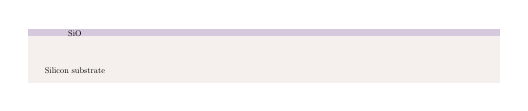
\begin{tikzpicture}[node distance = 3cm, auto, thick,scale=\CrossSectionOnly, every node/.style={transform shape}]
		% substrate
\fill[substrate] (0,0) rectangle (20,2);
\node at (2,0.5) {Silicon substrate};
% oxide
\fill[isolationoxide] (0,2) rectangle (20,2.3);
\node at (2,2.1) {SiO};
	\end{tikzpicture} \\
	
\includegraphics[scale=0.01]{down_arrow.png} \\
	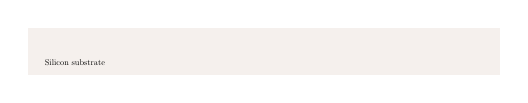
\begin{tikzpicture}[node distance = 3cm, auto, thick,scale=\CrossSectionOnly, every node/.style={transform shape}]
		% substrate
\fill[substrate] (0,0) rectangle (20,2);
\node at (2,0.5) {Silicon substrate};
	\end{tikzpicture}
	\caption{Initial cleaning}
	\label{initial_cleaning}
\end{figure}

This needs to be done because the naturally grown initially existing silicon oxide is not pure and may contain contamination which may render the final product unusable.

\subsubsection{Sulfuric Cleaning}
The sulfuric acid mixture, $H_2 S O_4 + H_2 O_2$ is being applied to the wafer for 10 minutes at a temperature of 120 \degree C.

\subsubsection{HF dip}
After the sulfuric cleaning a HF (HF:$H_2O$,1:50) dip is being performed for one minute. \\
Hydrofluoric acid (HF) is used to remove native silicon dioxide from wafers. Since it acts quickly, one needs to only expose the wafer for a short time ("dip").

\subsubsection{Drying}
After that the wafer needs to be dried and quickly processed further before new uncontrolled natural oxide can build up on the wafer through the contact with air.

\subsection{Hard mask: Oxide growth}
We need a thick layer of oxide as protective hard mask to etch the trenches into the silicon.

\begin{figure}[H]
	\centering
	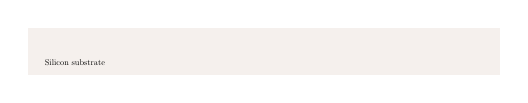
\begin{tikzpicture}[node distance = 3cm, auto, thick,scale=\CrossSectionOnly, every node/.style={transform shape}]
		% substrate
\fill[substrate] (0,0) rectangle (20,2);
\node at (2,0.5) {Silicon substrate};
	\end{tikzpicture} \\
	
\includegraphics[scale=0.01]{down_arrow.png} \\
	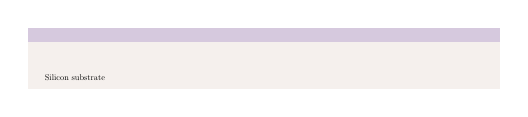
\begin{tikzpicture}[node distance = 3cm, auto, thick,scale=\CrossSectionOnly, every node/.style={transform shape}]
		% substrate
\fill[substrate] (0,0) rectangle (20,2);
\node at (2,0.5) {Silicon substrate};
\fill[isolationoxide] (0,2) rectangle (20,2.6);
	\end{tikzpicture}
	\caption{Hard mask growth}
\end{figure}

Because we want to etch 2\um deep into the silicon which takes 4 minutes and 30 seconds using KOH acid at 60\degreesC in \autoref{sti_trench_etch}.

This means the oxide layer needs to be at least 226 nm thick, so we choose a nice round number of 300nm.

The layer of silicon dioxide of around 300nm thickness is grown in wet ambient for 25 minutes at 1050\degreesC\footnote{\url{http://cleanroom.byu.edu/OxideTimeCalc}} in the diffusion furnace.

\newpage

\subsection{Hard mask: Patterning}

The resist is being deposited using spin coating and then baked depending on the baking time for the specific resist.

\begin{figure}[H]
	\centering
	\begin{tikzpicture}[node distance = 3cm, auto, thick,scale=\CrossSectionOnly, every node/.style={transform shape}]
		\input{tikz_process_steps/sti.hard_mask_oxide_growth.a.tex}
\fill[isolationoxide] (0,2) rectangle (20,2.6);
	\end{tikzpicture} \\
	
\includegraphics[scale=0.01]{down_arrow.png} \\
	\begin{tikzpicture}[node distance = 3cm, auto, thick,scale=\CrossSectionOnly, every node/.style={transform shape}]
		\input{tikz_process_steps/sti.hard_mask_oxide_growth.a.tex}
\fill[isolationoxide] (0,2) rectangle (20,2.6);
\fill[resist] (1,2.6) rectangle (8,3.2);
\fill[resist] (11.5,2.6) rectangle (19,3.2);
	\end{tikzpicture}
	\caption{Patterning with positive resist}
\end{figure}

The layout for being exposed onto the resist is being extracted from the "active" layer within the GDS2 file onto a dark field mask.

A dark field mask can be used because alignment doesn't play a role yet because it's the first layer, however the alignment crosses need to be included into the mask.

\subsection{Hard mask: Etching}\label{sti_mask_etch}

We open the access to the silicon outside of the active areas in order to etch the trenches.

\begin{figure}[H]
	\centering
	\begin{tikzpicture}[node distance = 3cm, auto, thick,scale=\CrossSectionOnly, every node/.style={transform shape}]
		\input{tikz_process_steps/sti.hard_mask_oxide_growth.b.tex}
\fill[resist] (1,2.6) rectangle (8,3.2);
\fill[resist] (11.5,2.6) rectangle (19,3.2);
	\end{tikzpicture} \\
	
\includegraphics[scale=0.01]{down_arrow.png} \\
	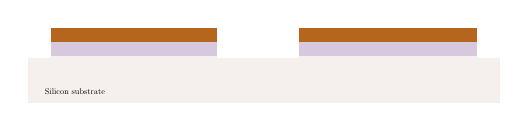
\begin{tikzpicture}[node distance = 3cm, auto, thick,scale=\CrossSectionOnly, every node/.style={transform shape}]
		% substrate
\fill[substrate] (0,0) rectangle (20,1.9);
\node at (2,0.5) {Silicon substrate};

% substrate islands
\fill[substrate] (1,1.9) rectangle (8,2);
\fill[substrate] (11.5,1.9) rectangle (19,2);

% pad oxide
\fill[isolationoxide] (1,2) rectangle (8,2.6);
\fill[isolationoxide] (11.5,2) rectangle (19,2.6);

% resist
\fill[resist] (1,2.6) rectangle (8,3.2);
\fill[resist] (11.5,2.6) rectangle (19,3.2);
	\end{tikzpicture}
	\caption{Nitride mask etching}
\end{figure}

There are dry etching and wet etching methods available for etching the oxide hard mask. The downside of wet etching is that it also etches horizontally, however the chemical BHF is readily available and allows for easy implementation of the process.\\

\textbf{Possible approaches}:
\begin{itemize}
	\item \textbf{"DRIE Etcher \#1" from HKUST} \\
	We can use anisotropic plasma etching for sharper borders.
	\item \textbf{Chemical solution} \\
	We can use buffered hydrofluoric acid (BOE (1:6)) at room temperature for a little bit over 3 minutes in order to get through the 300nm of oxide.\\
	Too long over 3 minutes might cause under-etch however!
\end{itemize}

\subsection{Hard mask: Resist removal}
Now we need to remove the contaminants for further processing.

\begin{figure}[H]
	\centering
	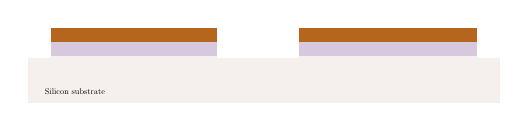
\begin{tikzpicture}[node distance = 3cm, auto, thick,scale=\CrossSectionOnly, every node/.style={transform shape}]
		% substrate
\fill[substrate] (0,0) rectangle (20,1.9);
\node at (2,0.5) {Silicon substrate};

% substrate islands
\fill[substrate] (1,1.9) rectangle (8,2);
\fill[substrate] (11.5,1.9) rectangle (19,2);

% pad oxide
\fill[isolationoxide] (1,2) rectangle (8,2.6);
\fill[isolationoxide] (11.5,2) rectangle (19,2.6);

% resist
\fill[resist] (1,2.6) rectangle (8,3.2);
\fill[resist] (11.5,2.6) rectangle (19,3.2);
	\end{tikzpicture} \\
	
\includegraphics[scale=0.01]{down_arrow.png} \\
	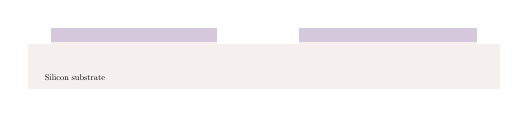
\begin{tikzpicture}[node distance = 3cm, auto, thick,scale=\CrossSectionOnly, every node/.style={transform shape}]
		% substrate
\fill[substrate] (0,0) rectangle (20,1.9);
\node at (2,0.5) {Silicon substrate};

% substrate islands
\fill[substrate] (1,1.9) rectangle (8,2);
\fill[substrate] (11.5,1.9) rectangle (19,2);

% pad oxide
\fill[isolationoxide] (1,2) rectangle (8,2.6);
\fill[isolationoxide] (11.5,2) rectangle (19,2.6);
	\end{tikzpicture}
	\caption{Resist removal}
\end{figure}

We strip the resist, rinse and perform sulfuric cleaning.

\newpage

\subsection{Silicon etching}\label{sti_trench_etch}

Silicon can only be etched by a very aggressive chemical cocktail of  KOH and TMAH (20\%) or by plasma etching.

\begin{figure}[H]
	\centering
	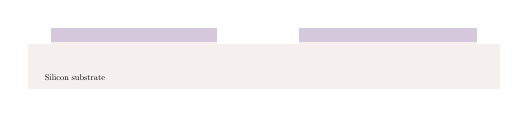
\begin{tikzpicture}[node distance = 3cm, auto, thick,scale=\CrossSectionOnly, every node/.style={transform shape}]
		% substrate
\fill[substrate] (0,0) rectangle (20,1.9);
\node at (2,0.5) {Silicon substrate};

% substrate islands
\fill[substrate] (1,1.9) rectangle (8,2);
\fill[substrate] (11.5,1.9) rectangle (19,2);

% pad oxide
\fill[isolationoxide] (1,2) rectangle (8,2.6);
\fill[isolationoxide] (11.5,2) rectangle (19,2.6);
	\end{tikzpicture} \\
	
\includegraphics[scale=0.01]{down_arrow.png} \\
	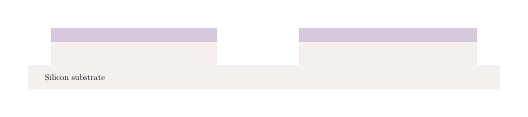
\begin{tikzpicture}[node distance = 3cm, auto, thick,scale=\CrossSectionOnly, every node/.style={transform shape}]
		% substrate
\fill[substrate] (0,0) rectangle (20,1);
\node at (2,0.5) {Silicon substrate};

% substrate islands
\fill[substrate] (1,1) rectangle (8,2);
\fill[substrate] (11.5,1) rectangle (19,2);

% pad oxide
\fill[isolationoxide] (1,2) rectangle (8,2.6);
\fill[isolationoxide] (11.5,2) rectangle (19,2.6);
	\end{tikzpicture}
	\caption{Trench etching}
\end{figure}

\textbf{Possible approaches}:
\begin{itemize}
\item \textbf{"DRIE Etcher \#1" from HKUST} \\
Has a normal etching rate of up to $2\frac{\mu m}{min}$.
This means we etch for 10 minutes with a reduced etch speed of $200\frac{nm}{min}$ in order to be clearly deep enough and to compensate for different etch depths in different places.
This way we have a good chance of having proper isolation everywhere on the wafer.

\item \textbf{Chemical solution} \\
Using a KOH solution of 20\% at 60\degreesC gives us an etch rate of roughly  26.57\um per hour\footnote{\url{http://www.lelandstanfordjunior.com/KOH.html}}.
\begin{itemize}
\item The <100> etch rate is: 26.57 micron/hr = 0.44 micron/min
\item The <110> etch rate is: 40.5 micron/hr 
\item The <111> etch rate is: 0.4932 micron/hr 
\item The SiO2 etch rate is: 49.92 nanometers/hr 
\end{itemize}
With a desired depth of 2\um we will have to etch around 4 minutes and 30 seconds in order to reach the desired depth.
The disadvantage of this approach is the imprecision and under-etch of the mask.
\end{itemize}

\subsection{Hard mask: Removal}

Now we have to remove the oxide hard mask for further processing in order to proceed with well formation without contamination during oxide growing.

\begin{figure}[H]
	\centering
	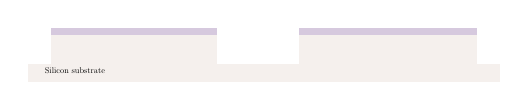
\begin{tikzpicture}[node distance = 3cm, auto, thick,scale=\CrossSectionOnly, every node/.style={transform shape}]
		% substrate
\fill[substrate] (0,0) rectangle (20,0.75);
\node at (2,0.5) {Silicon substrate};

% substrate islands
\fill[substrate] (1,0.75) rectangle (8,2);
\fill[substrate] (11.5,0.75) rectangle (19,2);

% covering oxide
\fill[isolationoxide] (1,2) rectangle (8,2.3);
\fill[isolationoxide] (11.5,2) rectangle (19,2.3);
	\end{tikzpicture} \\
	
\includegraphics[scale=0.01]{down_arrow.png} \\
	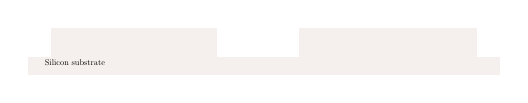
\begin{tikzpicture}[node distance = 3cm, auto, thick,scale=\CrossSectionOnly, every node/.style={transform shape}]
		% substrate
\fill[substrate] (0,0) rectangle (20,0.75);
\node at (2,0.5) {Silicon substrate};

% substrate islands
\fill[substrate] (1,0.75) rectangle (8,2);
\fill[substrate] (11.5,0.75) rectangle (19,2);
	\end{tikzpicture}
	\caption{Trench etching}
\end{figure}

We use buffered hydrofluoric acid (BOE (1:6)) at room temperature for a little bit over 3 minutes in order to remove all of the 300nm thick oxide layer.
\newpage
\section{N-well}\label{nwell_chapter}
In order to build CMOS on the same substrate, an N-well is required for building the complementary P-channel transistor for a n-p-channel logic circuitry as shown above in the example section.
The cross section as well as the top view of the targeted geometry are shown in \autoref{nwell_target}
\begin{figure}[H]
	\centering
	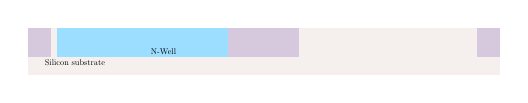
\begin{tikzpicture}[node distance = 3cm, auto, thick,scale=\CrossAndTopSectionBig, every node/.style={transform shape}]
		% substrate
\fill[substrate] (0,0) rectangle (20,2);
\node at (2,0.5) {Silicon substrate};
%trenches
\fill[isolationoxide] (0,0.75) rectangle (1,2);
\fill[isolationoxide] (8.5,0.75) rectangle (11.5,2);
\fill[isolationoxide] (19,0.75) rectangle (20,2);
% n-well
\fill[nwell] (1.25,0.75) rectangle (8.5,2);
\node at (5.75,1) {N-Well};


	\end{tikzpicture}
	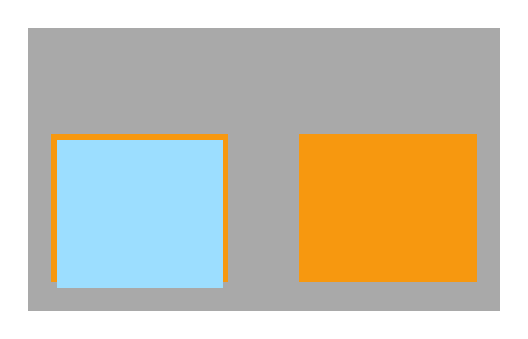
\begin{tikzpicture}[node distance = 3cm, auto, thick,scale=\CrossAndTopSectionBig, every node/.style={transform shape}]
		% substrate
\fill[YellowOrange] (0,0) rectangle (20,12);
% trench area
\fill[DarkGray] (0,0) rectangle (1,12);
\fill[DarkGray] (8.5,0) rectangle (11.5,12);
\fill[DarkGray] (19,0) rectangle (20,12);
\fill[DarkGray] (0,0) rectangle (20,1.25);
\fill[DarkGray] (0,7.5) rectangle (20,12);
\fill[nwell] (1.25,1) rectangle (8.25,7.25);
	\end{tikzpicture}
	\caption{N-well target geometry}
	\label{nwell_target}
\end{figure}

The N-well will serve us as an island of N-doped substrate within the P-doped basis substrate.

The dopant dose will be $2.5\times10^{12}cm^{-2}$ as calculated in the documentation of the process design leading to these steps\footnote{\url{https://github.com/leviathanch/libresiliconprocess/raw/master/process_design/process_design.pdf}}.

\begin{figure}[H]
	\centering
	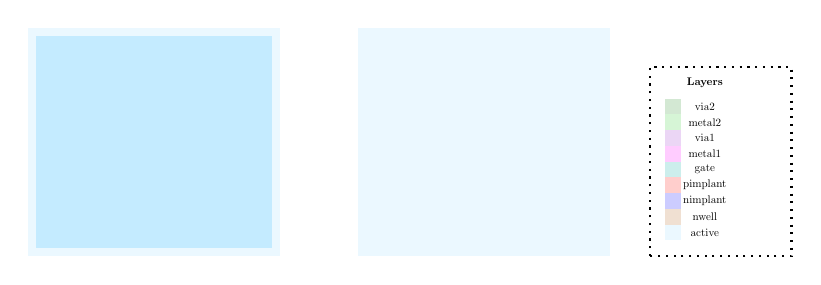
\begin{tikzpicture}[node distance =1cm, auto, thick,scale=\VLSILayout, every node/.style={transform shape}]
		\fill[nwell,opacity=0.2] (0.75,0.5) rectangle (8.75,7.75);
\fill[nwell,opacity=0.2] (11.25,0.5) rectangle (19.25,7.75);

\draw[dotted] (20.5,0.5) rectangle (25,6.5);

\node at (22.25,6) {\textbf{Layers}};

\fill[nwell,opacity=0.2] (21,1) rectangle (21.5,1.5);
\node at (22.25,1.25) {active};

\fill[resist,opacity=0.2] (21,1.5) rectangle (21.5,2);
\node at (22.25,1.75) {nwell};

\fill[blue,opacity=0.2] (21,2) rectangle (21.5,2.5);
\node at (22.25,2.25) {nimplant};

\fill[nitride,opacity=0.2] (21,2.5) rectangle (21.5,3);
\node at (22.25,2.75) {pimplant};

\fill[Emerald,opacity=0.2] (21,3) rectangle (21.5,3.5);
\node at (22.25,3.25) {gate};

\fill[Fuchsia,opacity=0.2] (21,3.5) rectangle (21.5,4);
\node at (22.25,3.75) {metal1};

\fill[DarkOrchid,opacity=0.2] (21,4) rectangle (21.5,4.5);
\node at (22.25,4.25) {via1};

\fill[LimeGreen,opacity=0.2] (21,4.5) rectangle (21.5,5);
\node at (22.25,4.75) {metal2};

\fill[ForestGreen,opacity=0.2] (21,5) rectangle (21.5,5.5);
\node at (22.25,5.25) {via2};

\fill[nwell,opacity=\OpacityLayout] (1,0.75) rectangle (8.5,7.5);
	\end{tikzpicture}
	\caption{N-Well layout}
	\label{nwell_layout}
\end{figure}

In \autoref{nwell_layout} the layout of the n-well region on top of the active area region can be seen.

The n-well is being fit into the active area. It should even be a little bit bigger than the active area, because of possible alignment offsets

\newpage

\subsection{Mask dioxide layer}
In order to selectively inject charge carrying atoms into the crystalline structure a protective dioxide ($SiO_2$) layer needs to be grown on top of a p-type substrate.
\begin{figure}[H]
	\centering
	\begin{tikzpicture}[node distance = 3cm, auto, thick,scale=\CrossSectionOnly, every node/.style={transform shape}]
		\input{tikz_process_steps/pwell.mask_dioxide_layer.a.tex}

% pwell
\fill[pwell] (11.75,0.75) rectangle (18.75,2);
\node at (14.25,1) {P-Well};
	\end{tikzpicture}
	\drawStepArrow{}
	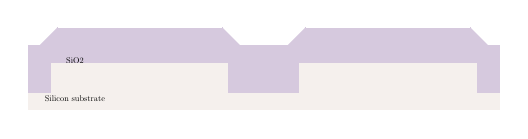
\begin{tikzpicture}[node distance = 3cm, auto, thick,scale=\CrossSectionOnly, every node/.style={transform shape}]
		% oxide
\fill[isolationoxide] (0,1.25) rectangle (20,2.75);

% oxide hill 1
\fill[isolationoxide] (1.25,2.75) rectangle (8.25,3.5);
\filldraw[line width=0, isolationoxide] (0.5,2.75) -- (1.25,2.75) -- (1.25,3.5);
\filldraw[line width=0, isolationoxide] (8.25,2.75) -- (8.25,3.5) -- (9.0,2.75);

% oxide hill 2
\fill[isolationoxide] (11.75,2.75) rectangle (18.75,3.5);
\filldraw[line width=0, isolationoxide] (11.0,2.75) -- (11.75,2.75) -- (11.75,3.5);
\filldraw[line width=0, isolationoxide] (18.75,2.75) -- (18.75,3.5) -- (19.5,2.75);

\node at (2,2.1) {SiO2};

% substrate
\fill[substrate] (0,0) rectangle (20,2);
\node at (2,0.5) {Silicon substrate};
%trenches
\fill[isolationoxide] (0,0.75) rectangle (1,2);
\fill[isolationoxide] (8.5,0.75) rectangle (11.5,2);
\fill[isolationoxide] (19,0.75) rectangle (20,2);
	\end{tikzpicture}
	\caption{Dioxide layer growth}
\end{figure}

With an energy of 100keV for the implantation performed in \autoref{nwell_implant_step}, the projected range of the dopants within the oxide will be 100nm (130nm tops) \footnote{\url{http://cleanroom.byu.edu/rangestraggle}}.
This means being on the safe side and having 300nm as the thickness is a good approach.

In order to grow the 300nm thick oxide layer, the wafer is being oxidized for around 25 minutes at 1050\degree C using wet oxidation which results in a dioxide layer of around 300nm in thickness\footnote{\url{http://cleanroom.byu.edu/OxideTimeCalc}}.

\subsection{Patterning}

The resist is being deposited using spray coating because the uneven nature of the oxide layer.
After that the wafer is being soft baked depending on the baking time and temperature for the specific resist.
The layout for being exposed onto the resist is being extracted from the "nwell" layer within the GDS2 file onto a \textbf{bright field} mask.
The requirement is a \textbf{negative} tone resist.

\begin{figure}[H]
	\centering
	\begin{tikzpicture}[node distance = 3cm, auto, thick,scale=\CrossAndTopSection, every node/.style={transform shape}]
		% oxide
\fill[isolationoxide] (0,1.25) rectangle (20,2.75);

% oxide hill 1
\fill[isolationoxide] (1.25,2.75) rectangle (8.25,3.5);
\filldraw[line width=0, isolationoxide] (0.5,2.75) -- (1.25,2.75) -- (1.25,3.5);
\filldraw[line width=0, isolationoxide] (8.25,2.75) -- (8.25,3.5) -- (9.0,2.75);

% oxide hill 2
\fill[isolationoxide] (11.75,2.75) rectangle (18.75,3.5);
\filldraw[line width=0, isolationoxide] (11.0,2.75) -- (11.75,2.75) -- (11.75,3.5);
\filldraw[line width=0, isolationoxide] (18.75,2.75) -- (18.75,3.5) -- (19.5,2.75);

\node at (2,2.1) {SiO2};

\input{tikz_process_steps/sti.a.tex}
	\end{tikzpicture}
	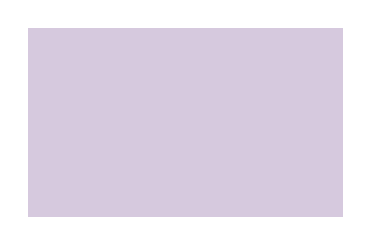
\begin{tikzpicture}[node distance = 3cm, auto, thick,scale=\CrossAndTopSection, every node/.style={transform shape}]
		% resist
\fill[isolationoxide] (0,0) rectangle (20,12);
	\end{tikzpicture}
	\drawStepArrow{Mask: nwell}
	\begin{tikzpicture}[node distance = 3cm, auto, thick,scale=\CrossAndTopSection, every node/.style={transform shape}]
		% resist
\fill[resist] (0,2.6) rectangle (1,5.0);
\fill[resist] (8.5,2.6) rectangle (20,5.0);

% oxide
\fill[isolationoxide] (0,1.25) rectangle (20,2.75);

% oxide hill 1
\fill[isolationoxide] (1.25,2.75) rectangle (8.25,3.5);
\filldraw[line width=0, isolationoxide] (0.5,2.75) -- (1.25,2.75) -- (1.25,3.5);
\filldraw[line width=0, isolationoxide] (8.25,2.75) -- (8.25,3.5) -- (9.0,2.75);

% oxide hill 2
\fill[isolationoxide] (11.75,2.75) rectangle (18.75,3.5);
\filldraw[line width=0, isolationoxide] (11.0,2.75) -- (11.75,2.75) -- (11.75,3.5);
\filldraw[line width=0, isolationoxide] (18.75,2.75) -- (18.75,3.5) -- (19.5,2.75);

\node at (2,2.1) {SiO2};

\input{tikz_process_steps/sti.a.tex}
	\end{tikzpicture}
	
\begin{tikzpicture}[node distance = 3cm, auto, thick,scale=\CrossAndTopSection, every node/.style={transform shape}]
		% resist
\fill[resist] (0,0) rectangle (20,12);
% substrate
\fill[isolationoxide] (1.25,1.5) rectangle (8.25,7.25);
	\end{tikzpicture}
	\caption{Cross/top view of n-well layout on resist}
\end{figure}

The thickness of the resist layer and the baking duration will variate depending on the specific equipment for which this process will be implemented with.
Also after the exposure and development, the hard baking shouldn't be forgotten!

\newpage

\subsection{Etching}
We now need to open a window in the dioxide layer, through which we will inject carrier atoms into the silicon crystal structure.
\begin{figure}[H]
	\centering
	\begin{tikzpicture}[node distance = 3cm, auto, thick,scale=\CrossAndTopSection, every node/.style={transform shape}]
		% resist
\fill[resist] (0,2.6) rectangle (1,5.0);
\fill[resist] (8.5,2.6) rectangle (20,5.0);

\input{tikz_process_steps/nwell.mask_dioxide_layer.b.tex}
	\end{tikzpicture}
	
\begin{tikzpicture}[node distance = 3cm, auto, thick,scale=\CrossAndTopSection, every node/.style={transform shape}]
		% resist
\fill[resist] (0,0) rectangle (20,12);
% substrate
\fill[isolationoxide]  (1,0.75) rectangle (8.5,7.5);
	\end{tikzpicture}
	\drawStepArrow{}
	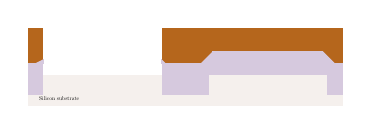
\begin{tikzpicture}[node distance = 3cm, auto, thick,scale=\CrossAndTopSection, every node/.style={transform shape}]
		% resist
\fill[resist] (0,2.6) rectangle (1,5.0);
\fill[resist] (8.5,2.6) rectangle (20,5.0);

% oxide
\fill[isolationoxide] (0,1.25) rectangle (1,2.75);
\fill[isolationoxide] (8.5,1.25) rectangle (20,2.75);

% oxide hill 1
\filldraw[line width=0, isolationoxide] (0.5,2.75) -- (1.0,2.75) -- (1.0,3.0);
\filldraw[line width=0, isolationoxide] (8.75,2.75) -- (8.5,2.75) -- (8.5,3.0);

% oxide hill 2
\fill[isolationoxide] (11.75,2.75) rectangle (18.75,3.5);
\filldraw[line width=0, isolationoxide] (11.0,2.75) -- (11.75,2.75) -- (11.75,3.5);
\filldraw[line width=0, isolationoxide] (18.75,2.75) -- (18.75,3.5) -- (19.5,2.75);

% substrate
\fill[substrate] (0,0) rectangle (20,2);
\node at (2,0.5) {Silicon substrate};
%trenches
\fill[isolationoxide] (0,0.75) rectangle (1,2);
\fill[isolationoxide] (8.5,0.75) rectangle (11.5,2);
\fill[isolationoxide] (19,0.75) rectangle (20,2);
	\end{tikzpicture}
	
\begin{tikzpicture}[node distance = 3cm, auto, thick,scale=\CrossAndTopSection, every node/.style={transform shape}]
		% resist
\fill[resist] (0,0) rectangle (20,12);
% substrate
\fill[substrate] (1.25,1) rectangle (8.25,7.25);
	\end{tikzpicture}
	\caption{Cross/top view of n-well oxide window}
\end{figure}

Since the silicon dioxide layer is 300nm thick and we wanna reach the silicon below we can use wet etching as described in the chemistry chapter.\\

\textbf{Possible approaches}:
\begin{itemize}
	\item \textbf{"AOE Etcher (DRY-AOE)" from HKUST} \\
	We can use anisotropic plasma etching for sharper borders.
	\item \textbf{Chemical solution} \\
	We can use buffered hydrofluoric acid (BOE (1:6)) at room temperature for a little bit over 3 minutes in order to get through the 300nm of oxide.\\
	Too long over 3 minutes might cause under-etch however!
\end{itemize}

\subsection{Cleaning}
In order to avoid contamination of the machines we need to make sure all the resist has been stripped off from the wafer.
\begin{figure}[H]
	\centering
	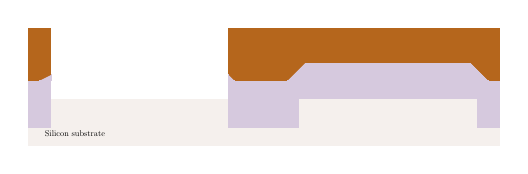
\begin{tikzpicture}[node distance = 3cm, auto, thick,scale=\CrossSectionOnly, every node/.style={transform shape}]
		% resist
\fill[resist] (0,2.6) rectangle (1,5.0);
\fill[resist] (8.5,2.6) rectangle (20,5.0);

% oxide
\fill[isolationoxide] (0,1.25) rectangle (1,2.75);
\fill[isolationoxide] (8.5,1.25) rectangle (20,2.75);

% oxide hill 1
\filldraw[line width=0, isolationoxide] (0.5,2.75) -- (1.0,2.75) -- (1.0,3.0);
\filldraw[line width=0, isolationoxide] (8.75,2.75) -- (8.5,2.75) -- (8.5,3.0);

% oxide hill 2
\fill[isolationoxide] (11.75,2.75) rectangle (18.75,3.5);
\filldraw[line width=0, isolationoxide] (11.0,2.75) -- (11.75,2.75) -- (11.75,3.5);
\filldraw[line width=0, isolationoxide] (18.75,2.75) -- (18.75,3.5) -- (19.5,2.75);

% substrate
\fill[substrate] (0,0) rectangle (20,2);
\node at (2,0.5) {Silicon substrate};
%trenches
\fill[isolationoxide] (0,0.75) rectangle (1,2);
\fill[isolationoxide] (8.5,0.75) rectangle (11.5,2);
\fill[isolationoxide] (19,0.75) rectangle (20,2);
	\end{tikzpicture}
	\drawStepArrow{}
	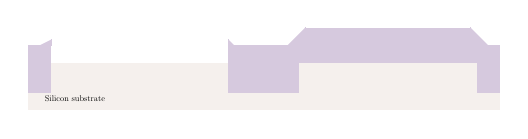
\begin{tikzpicture}[node distance = 3cm, auto, thick,scale=\CrossSectionOnly, every node/.style={transform shape}]
		% oxide
\fill[isolationoxide] (0,1.25) rectangle (1,2.75);
\fill[isolationoxide] (8.5,1.25) rectangle (20,2.75);

% oxide hill 1
\filldraw[line width=0, isolationoxide] (0.5,2.75) -- (1.0,2.75) -- (1.0,3.0);
\filldraw[line width=0, isolationoxide] (8.75,2.75) -- (8.5,2.75) -- (8.5,3.0);

% oxide hill 2
\fill[isolationoxide] (11.75,2.75) rectangle (18.75,3.5);
\filldraw[line width=0, isolationoxide] (11.0,2.75) -- (11.75,2.75) -- (11.75,3.5);
\filldraw[line width=0, isolationoxide] (18.75,2.75) -- (18.75,3.5) -- (19.5,2.75);

% substrate
\fill[substrate] (0,0) rectangle (20,2);
\node at (2,0.5) {Silicon substrate};
%trenches
\fill[isolationoxide] (0,0.75) rectangle (1,2);
\fill[isolationoxide] (8.5,0.75) rectangle (11.5,2);
\fill[isolationoxide] (19,0.75) rectangle (20,2);
	\end{tikzpicture}
	\caption{Resist removal}
\end{figure}
Please just use the solvent for the specific resist.

\newpage

\subsection{Implantation/Doping}\label{nwell_implant_step}
We now need to inject the carriers into the upper level of the n-channel area so that we can later on drive them into the crystal during the drive-in step.

\begin{figure}[H]
	\centering
	\begin{minipage}{0.5\textwidth}
	\centering
	\begin{tikzpicture}[node distance = 3cm, auto, thick,scale=\CrossSectionOnly, every node/.style={transform shape}]
		% oxide
\fill[isolationoxide] (0,1.25) rectangle (1,2.75);
\fill[isolationoxide] (8.5,1.25) rectangle (20,2.75);

% oxide hill 1
\filldraw[line width=0, isolationoxide] (0.5,2.75) -- (1.0,2.75) -- (1.0,3.0);
\filldraw[line width=0, isolationoxide] (8.75,2.75) -- (8.5,2.75) -- (8.5,3.0);

% oxide hill 2
\fill[isolationoxide] (11.75,2.75) rectangle (18.75,3.5);
\filldraw[line width=0, isolationoxide] (11.0,2.75) -- (11.75,2.75) -- (11.75,3.5);
\filldraw[line width=0, isolationoxide] (18.75,2.75) -- (18.75,3.5) -- (19.5,2.75);

\input{tikz_process_steps/sti.a.tex}

\forloop{ct}{0}{\value{ct} < 21}
{
	\draw [->] (\value{ct},5) -- (\value{ct},4);
	\node at (\value{ct},5.2) {P$^{31}$};
}
	\end{tikzpicture}
	\drawStepArrow{Boron implant}
	\begin{tikzpicture}[node distance = 3cm, auto, thick,scale=\CrossSectionOnly, every node/.style={transform shape}]
		% resist
\fill[resist] (0.25,2.0) rectangle (1,5.0);
\fill[resist] (8.5,2.0) rectangle (19.75,5.0);

% oxide
\fill[isolationoxide] (0,1.25) rectangle (1,2.75);
\fill[isolationoxide] (8.5,1.25) rectangle (20,2.75);

% oxide hill 1
\filldraw[line width=0, isolationoxide] (0.5,2.75) -- (1.0,2.75) -- (1.0,3.0);
\filldraw[line width=0, isolationoxide] (8.75,2.75) -- (8.5,2.75) -- (8.5,3.0);

% oxide hill 2
\fill[isolationoxide] (11.75,2.75) rectangle (18.75,3.5);
\filldraw[line width=0, isolationoxide] (11.0,2.75) -- (11.75,2.75) -- (11.75,3.5);
\filldraw[line width=0, isolationoxide] (18.75,2.75) -- (18.75,3.5) -- (19.5,2.75);

\input{tikz_process_steps/sti.a.tex}

	\end{tikzpicture}
	\drawStepArrow{Annealing}
	\begin{tikzpicture}[node distance = 3cm, auto, thick,scale=\CrossSectionOnly, every node/.style={transform shape}]
		% oxide
\fill[isolationoxide] (0,1.25) rectangle (1,2.75);
\fill[isolationoxide] (8.5,1.25) rectangle (20,2.75);

% oxide hill 1
\filldraw[line width=0, isolationoxide] (0.5,2.75) -- (1.0,2.75) -- (1.0,3.0);
\filldraw[line width=0, isolationoxide] (8.75,2.75) -- (8.5,2.75) -- (8.5,3.0);

% oxide hill 2
\fill[isolationoxide] (11.75,2.75) rectangle (18.75,3.5);
\filldraw[line width=0, isolationoxide] (11.0,2.75) -- (11.75,2.75) -- (11.75,3.5);
\filldraw[line width=0, isolationoxide] (18.75,2.75) -- (18.75,3.5) -- (19.5,2.75);

\input{tikz_process_steps/sti.a.tex}
\shade[upper left = nwell, upper right = nwell, lower right = substrate, lower left = substrate,] (1.25,1.5) rectangle (8.25,2.0);
\shade[upper left = pwell, upper right = pwell, lower right = substrate, lower left = substrate,] (11.75,1.0) rectangle (18.75,2.0);
	\end{tikzpicture} \\
	\textbf{Implantation approach}
	\end{minipage}\begin{minipage}{0.5\textwidth}
	\centering
	\begin{tikzpicture}[node distance = 3cm, auto, thick,scale=\CrossSectionOnly, every node/.style={transform shape}]
		\fill[nwell] (0,0) rectangle (20,5);

% oxide
\fill[isolationoxide] (0,1.25) rectangle (1,2.75);
\fill[isolationoxide] (8.5,1.25) rectangle (20,2.75);

% oxide hill 1
\filldraw[line width=0, isolationoxide] (0.5,2.75) -- (1.0,2.75) -- (1.0,3.0);
\filldraw[line width=0, isolationoxide] (8.75,2.75) -- (8.5,2.75) -- (8.5,3.0);

% oxide hill 2
\fill[isolationoxide] (11.75,2.75) rectangle (18.75,3.5);
\filldraw[line width=0, isolationoxide] (11.0,2.75) -- (11.75,2.75) -- (11.75,3.5);
\filldraw[line width=0, isolationoxide] (18.75,2.75) -- (18.75,3.5) -- (19.5,2.75);

\input{tikz_process_steps/sti.a.tex}
	\end{tikzpicture}
	\drawStepArrow{Constant source diffusion}
	\begin{tikzpicture}[node distance = 3cm, auto, thick,scale=\CrossSectionOnly, every node/.style={transform shape}]
		\fill[nwell] (0,0) rectangle (20,5);

% oxide
\fill[isolationoxide] (0,1.25) rectangle (1,2.75);
\fill[isolationoxide] (8.5,1.25) rectangle (20,2.75);

% oxide hill 1
\filldraw[line width=0, isolationoxide] (0.5,2.75) -- (1.0,2.75) -- (1.0,3.0);
\filldraw[line width=0, isolationoxide] (8.75,2.75) -- (8.5,2.75) -- (8.5,3.0);

% oxide hill 2
\fill[isolationoxide] (11.75,2.75) rectangle (18.75,3.5);
\filldraw[line width=0, isolationoxide] (11.0,2.75) -- (11.75,2.75) -- (11.75,3.5);
\filldraw[line width=0, isolationoxide] (18.75,2.75) -- (18.75,3.5) -- (19.5,2.75);

\input{tikz_process_steps/sti.a.tex}

\shade[upper left = nwell, upper right = nwell, lower right = substrate, lower left = substrate,] (1.25,1.5) rectangle (8.25,2.0);
\shade[upper left = pwell, upper right = pwell, lower right = substrate, lower left = substrate,] (11.75,1.0) rectangle (18.75,2.0);
	\end{tikzpicture}
	\drawStepArrow{Source removal}
	\begin{tikzpicture}[node distance = 3cm, auto, thick,scale=\CrossSectionOnly, every node/.style={transform shape}]
		% oxide
\fill[isolationoxide] (0,1.25) rectangle (1,2.75);
\fill[isolationoxide] (8.5,1.25) rectangle (20,2.75);

% oxide hill 1
\filldraw[line width=0, isolationoxide] (0.5,2.75) -- (1.0,2.75) -- (1.0,3.0);
\filldraw[line width=0, isolationoxide] (8.75,2.75) -- (8.5,2.75) -- (8.5,3.0);

% oxide hill 2
\fill[isolationoxide] (11.75,2.75) rectangle (18.75,3.5);
\filldraw[line width=0, isolationoxide] (11.0,2.75) -- (11.75,2.75) -- (11.75,3.5);
\filldraw[line width=0, isolationoxide] (18.75,2.75) -- (18.75,3.5) -- (19.5,2.75);

\input{tikz_process_steps/sti.a.tex}

\shade[upper left = nwell, upper right = nwell, lower right = substrate, lower left = substrate,] (1.25,1.5) rectangle (8.25,2.0);
\shade[upper left = pwell, upper right = pwell, lower right = substrate, lower left = substrate,] (11.75,1.0) rectangle (18.75,2.0);
	\end{tikzpicture} \\
	\textbf{Diffusion approach}
	\end{minipage}
	\caption{Doping process}
\end{figure}


\textbf{Possible approaches}:
\begin{itemize}
	\item \textbf{"CF-3000 Implanter (IMP-3000)" from HKUST} \\
	At HKUST we have an implanter which gives us better control over the initial surface concentration. \\
	These steps are needed to arrive with the desired geometry:
	\begin{enumerate}
		\item Preparing by default cleaning
		\item The N-well is implanted with a Phosphorus ($P^{31}$) dose of $2.5\times10^{12}cm^{-2}$ at an energy of 100 keV.
		\item The N-well is annealed for 30 minutes at 1050\degreesC in $N_2$ environment (DIF-A1)\\
		After that the P-well will be around 2\um deep and the N-Well around 1\um deep
	\end{enumerate}
	\item \textbf{Constant source diffusion} \\
	We can add a layer of Phosphorus solution and diffusing in order to have an initial concentration in order to reach the desired concentration later by main diffusion.
		\begin{enumerate}
		\item A constant source is added (gas or liquid)
		\item The source dopant is driven in for 10 minutes at 1050\degreesC
		\item The dopant source is removed by stopping the gas flow or cleaning the surface
	\end{enumerate}
\end{itemize}

\newpage

\subsection{Oxide for drive-in}

Now we need to cover the now doped and annealed area with an oxide layer in order to seal it off and prevent the dopants from diffusing out of the crystal during the drive-in phase.

\begin{figure}[H]
	\centering
	\begin{tikzpicture}[node distance = 3cm, auto, thick,scale=\CrossSectionOnly, every node/.style={transform shape}]
		% resist
\fill[resist] (0.25,2.0) rectangle (1,5.0);
\fill[resist] (8.5,2.0) rectangle (19.75,5.0);

\input{tikz_process_steps/nwell.cleaning.b.tex}

	\end{tikzpicture}
	\drawStepArrow{}
	\begin{tikzpicture}[node distance = 3cm, auto, thick,scale=\CrossSectionOnly, every node/.style={transform shape}]
		\fill[isolationoxide] (0,0) rectangle (20,2.25);
\input{tikz_process_steps/nwell.cleaning.b.tex}
\shade[upper left = nwell, upper right = nwell, lower right = substrate, lower left = substrate,] (1.25,1.5) rectangle (8.25,2.0);
\shade[upper left = pwell, upper right = pwell, lower right = substrate, lower left = substrate,] (11.75,1.0) rectangle (18.75,2.0);
	\end{tikzpicture}
	\caption{Oxide growth}
\end{figure}

The wafer is being oxidized for around 5 minutes at 1050\degree C in a wet environment in order to achieve a cover silicon layer of around 90nm thickness.

\subsection{Drive-in}
In order to drive the carrier atoms deeper into the crystalline structure the wafer needs to be driven in after predeposition.

\begin{figure}[H]
	\centering
	\begin{tikzpicture}[node distance = 3cm, auto, thick,scale=\CrossSectionOnly, every node/.style={transform shape}]
		\fill[isolationoxide] (0,0) rectangle (20,2.25);
\input{tikz_process_steps/nwell.implantation.c.tex}
	\end{tikzpicture}
	\drawStepArrow{}
	\begin{tikzpicture}[node distance = 3cm, auto, thick,scale=\CrossSectionOnly, every node/.style={transform shape}]
		\fill[isolationoxide] (0,0) rectangle (20,2.25);
% resist
\fill[resist] (0.25,2.0) rectangle (1,5.0);
\fill[resist] (8.5,2.0) rectangle (19.75,5.0);

\input{tikz_process_steps/nwell.cleaning.b.tex}


% n-well
\fill[nwell] (1.25,0.75) rectangle (8.25,2);
\node at (4.75,1) {N-Well};

\fill[pwell] (11.75,0.75) rectangle (18.75,2);
\node at (15.25,1) {P-Well};
	\end{tikzpicture}
	\caption{Drive-in process}
\end{figure}

In this step the wafer is  driven-in for 90 minutes at 1050\degree C in an inert ambient\footnote{\url{http://cleanroom.byu.edu/DopConCalc}}

\subsection{Oxide mask removal}
Now we want to remove the silicon mask from the wafer and clean it for another clean oxide mask layer.

\begin{figure}[H]
	\centering
	\begin{tikzpicture}[node distance = 3cm, auto, thick,scale=\CrossSectionOnly, every node/.style={transform shape}]
		\fill[isolationoxide] (0,0) rectangle (20,2.25);
% resist
\fill[resist] (0.25,2.0) rectangle (1,5.0);
\fill[resist] (8.5,2.0) rectangle (19.75,5.0);

\input{tikz_process_steps/nwell.cleaning.b.tex}


% n-well
\fill[nwell] (1.25,0.75) rectangle (8.25,2);
\node at (4.75,1) {N-Well};

\fill[pwell] (11.75,0.75) rectangle (18.75,2);
\node at (15.25,1) {P-Well};
	\end{tikzpicture}
	\drawStepArrow{}
	\begin{tikzpicture}[node distance = 3cm, auto, thick,scale=\CrossSectionOnly, every node/.style={transform shape}]
		% substrate
\fill[substrate] (0,0) rectangle (20,2);
\node at (2,0.5) {Silicon substrate};
%trenches
\fill[isolationoxide] (0,0.75) rectangle (1,2);
\fill[isolationoxide] (8.5,0.75) rectangle (11.5,2);
\fill[isolationoxide] (19,0.75) rectangle (20,2);

% n-well
\fill[nwell] (1.25,0.75) rectangle (8.25,2);
\node at (4.75,1) {N-Well};
	\end{tikzpicture}
	\caption{Oxide removal}
\end{figure}

We use buffered hydrofluoric acid (BOE (1:6)) at room temperature for 3 minutes in order to remove the 300nm of oxide layer.
\newpage
`\section{P-well}\label{pwell_chapter}
In order to build CMOS on the same substrate, a P-well is required for building the complementary N-channel transistor for a n-p-channel logic circuitry.
The cross section as well as the top view of the targeted geometry are shown in \autoref{nwell_target}
\begin{figure}[H]
	\centering
	\begin{tikzpicture}[node distance = 3cm, auto, thick,scale=\CrossAndTopSectionBig, every node/.style={transform shape}]
		\input{tikz_process_steps/sti.a.tex}
% n-well
\fill[nwell] (1.25,0.75) rectangle (8.5,2);
\node at (5.75,1) {N-Well};


% p-well
\fill[pwell] (11.75,0.75) rectangle (18.75,2);
\node at (14.25,1) {P-Well};
	\end{tikzpicture}
	\begin{tikzpicture}[node distance = 3cm, auto, thick,scale=\CrossAndTopSectionBig, every node/.style={transform shape}]
		\input{tikz_process_steps/sti.b.tex}
\fill[nwell] (1.25,1) rectangle (8.25,7.25);
\fill[pwell] (11.75,1) rectangle (18.75,7.25);
	\end{tikzpicture}
	\caption{P-well target geometry}
	\label{pwell_target}
\end{figure}
The P-well will serve us as an island of higher p-doped substrate within the slightly p-doped basis substrate.

The dopant dose will be $2.5\times10^{12}cm^{-2}$ as calculated in the documentation of the process design leading to these steps\footnote{\url{https://github.com/leviathanch/libresiliconprocess/raw/master/process_design/process_design.pdf}}.

\begin{figure}[H]
	\centering
	\begin{tikzpicture}[node distance =1cm, auto, thick,scale=\VLSILayout, every node/.style={transform shape}]
		\input{tikz_process_steps/sti.layout.tex}
\fill[nwell,opacity=\OpacityLayout] (1,0.75) rectangle (8.5,7.5);
\fill[pwell,opacity=\OpacityLayout] (11.5,0.75) rectangle (19,7.5);
	\end{tikzpicture}
	\caption{P-Well layout}
	\label{pwell_layout}
\end{figure}

In \autoref{pwell_layout} the layout of the P-well region on top of the active area region can be seen.

The p-well is being fit into the active area.

It should even be a little bit bigger than the active area, because of possible alignment offsets

\newpage

\subsection{Mask dioxide layer}
In order to selectively inject charge carrying atoms into the crystalline structure a protective dioxide ($SiO_2$) layer needs to be grown on top of a p-type substrate.
\begin{figure}[H]
	\centering
	\begin{tikzpicture}[node distance = 3cm, auto, thick,scale=\CrossSectionOnly, every node/.style={transform shape}]
		\input{tikz_process_steps/sti.a.tex}
% n-well
\fill[nwell] (1.25,0.75) rectangle (8.5,2);
\node at (5.75,1) {N-Well};


	\end{tikzpicture} \\
	
\includegraphics[scale=0.01]{down_arrow.png} \\
	\begin{tikzpicture}[node distance = 3cm, auto, thick,scale=\CrossSectionOnly, every node/.style={transform shape}]
		% oxide
\fill[isolationoxide] (0,1.25) rectangle (20,2.75);

% oxide hill 1
\fill[isolationoxide] (1.25,2.75) rectangle (8.25,3.5);
\filldraw[line width=0, isolationoxide] (0.5,2.75) -- (1.25,2.75) -- (1.25,3.5);
\filldraw[line width=0, isolationoxide] (8.25,2.75) -- (8.25,3.5) -- (9.0,2.75);

% oxide hill 2
\fill[isolationoxide] (11.75,2.75) rectangle (18.75,3.5);
\filldraw[line width=0, isolationoxide] (11.0,2.75) -- (11.75,2.75) -- (11.75,3.5);
\filldraw[line width=0, isolationoxide] (18.75,2.75) -- (18.75,3.5) -- (19.5,2.75);

\node at (2,2.1) {SiO2};

\input{tikz_process_steps/nwell.a.tex}
	\end{tikzpicture}
	\caption{Dioxide layer growth}
\end{figure}
With an energy of 100keV for the implantation performed in \autoref{pwell_implant_step}, the projected range of the dopants within the oxide will be 310nm (380nm tops) \footnote{\url{http://cleanroom.byu.edu/rangestraggle}}.
This means being on the safe side and having 500nm as the thickness is a good approach.

In order to grow the 500nm thick oxide layer, the wafer is being oxidized for around 56 minutes at 1050\degree C using wet oxidation which results in a dioxide layer of around 500nm in thickness\footnote{\url{http://cleanroom.byu.edu/OxideTimeCalc}}.

\subsection{Patterning}
The resist is being deposited spray or spin coating (spray coating is better because of the uneven surface!) and then soft baked depending on the baking time for the specific resist.
The layout for being exposed onto the resist is being extracted from the "pwell" layer within the GDS2 file onto a \textbf{bright field} mask.
The requirement is a \textbf{negative} tone resist.

\begin{figure}[H]
	\centering
	\begin{tikzpicture}[node distance = 3cm, auto, thick,scale=\CrossAndTopSection, every node/.style={transform shape}]
		% oxide
\fill[isolationoxide] (0,1.25) rectangle (20,2.75);

% oxide hill 1
\fill[isolationoxide] (1.25,2.75) rectangle (8.25,3.5);
\filldraw[line width=0, isolationoxide] (0.5,2.75) -- (1.25,2.75) -- (1.25,3.5);
\filldraw[line width=0, isolationoxide] (8.25,2.75) -- (8.25,3.5) -- (9.0,2.75);

% oxide hill 2
\fill[isolationoxide] (11.75,2.75) rectangle (18.75,3.5);
\filldraw[line width=0, isolationoxide] (11.0,2.75) -- (11.75,2.75) -- (11.75,3.5);
\filldraw[line width=0, isolationoxide] (18.75,2.75) -- (18.75,3.5) -- (19.5,2.75);

\node at (2,2.1) {SiO2};

\input{tikz_process_steps/pwell.mask_dioxide_layer.a.tex}
	\end{tikzpicture}
	\begin{tikzpicture}[node distance = 3cm, auto, thick,scale=\CrossAndTopSection, every node/.style={transform shape}]
		% resist
\fill[isolationoxide] (0,0) rectangle (20,12);
	\end{tikzpicture} \\
	
\includegraphics[scale=0.01]{down_arrow.png} \\
	\begin{tikzpicture}[node distance = 3cm, auto, thick,scale=\CrossAndTopSection, every node/.style={transform shape}]
		% resist
\fill[resist] (0.25,2.0) rectangle (11.5,5.0);
\fill[resist] (19,2.0) rectangle (19.75,5.0);

\input{tikz_process_steps/pwell.mask_dioxide_layer.b.tex}

	\end{tikzpicture}
	\begin{tikzpicture}[node distance = 3cm, auto, thick,scale=\CrossAndTopSection, every node/.style={transform shape}]
		% resist
\fill[resist] (0,0) rectangle (20,12);
% substrate
\fill[isolationoxide] (11.5,1.5) rectangle (19,7.25);
	\end{tikzpicture}
	\caption{Cross/top view of P-well layout on resist}
\end{figure}
The thickness of the resist layer and the baking duration will variate depending on the specific equipment for which this process will be implemented with.
Also after the exposure and development, the hard baking shouldn't be forgotten!

\newpage

\subsection{Etching}
We now need to open a window in the dioxide layer, through which we will inject carrier atoms into the silicon crystal structure.
\begin{figure}[H]
	\centering
	\begin{tikzpicture}[node distance = 3cm, auto, thick,scale=\CrossAndTopSection, every node/.style={transform shape}]
		% resist
\fill[resist] (0.25,2.0) rectangle (11.5,5.0);
\fill[resist] (19,2.0) rectangle (19.75,5.0);

\input{tikz_process_steps/pwell.patterning.a.tex}

	\end{tikzpicture}
	\begin{tikzpicture}[node distance = 3cm, auto, thick,scale=\CrossAndTopSection, every node/.style={transform shape}]
		% resist
\fill[resist] (0,0) rectangle (20,12);
% substrate
\fill[isolationoxide] (1.25,1.5) rectangle (8.25,7.25);
	\end{tikzpicture} \\
	
\includegraphics[scale=0.01]{down_arrow.png} \\
	\begin{tikzpicture}[node distance = 3cm, auto, thick,scale=\CrossAndTopSection, every node/.style={transform shape}]
		% resist
\fill[resist] (0,2.6) rectangle (11.5,5.0);
\fill[resist] (19,2.6) rectangle (20,5.0);

% oxide
\fill[isolationoxide] (0,1.25) rectangle (11.5,2.75);
\fill[isolationoxide] (19,1.25) rectangle (20,2.75);

% oxide hill 1
\fill[isolationoxide] (1.25,2.75) rectangle (8.25,3.5);
\filldraw[line width=0, isolationoxide] (0.5,2.75) -- (1.25,2.75) -- (1.25,3.5);
\filldraw[line width=0, isolationoxide] (8.25,2.75) -- (8.25,3.5) -- (9.0,2.75);

% oxide hill 2
\filldraw[line width=0, isolationoxide] (11.25,2.75) -- (11.5,2.75) -- (11.5,3.0);
\filldraw[line width=0, isolationoxide] (19.0,3.0)  -- (19.0,2.75) -- (19.00,2.75);

\node at (2,2.1) {SiO2};

\input{tikz_process_steps/nwell.a.tex}


	\end{tikzpicture}
	\begin{tikzpicture}[node distance = 3cm, auto, thick,scale=\CrossAndTopSection, every node/.style={transform shape}]
		% resist
\fill[resist] (0,0) rectangle (20,12);
% substrate
\fill[substrate] (1.25,1.5) rectangle (8.25,7.25);
	\end{tikzpicture}
	\caption{Cross/top view of P-well oxide window}
\end{figure}

There are multiple possible approaches to etch through these 500nm of oxide.\\

\textbf{Possible approaches}:
\begin{itemize}
	\item \textbf{"AOE Etcher (DRY-AOE)" from HKUST} \\
	We can use anisotropic plasma etching for sharper borders.
	\item \textbf{Chemical solution} \\
	We can use buffered hydrofluoric acid (BOE (1:6)) at room temperature for 5 minutes in order to get through the 500nm of oxide.\\
	Too long over 4 minutes might cause under-etch however!
\end{itemize}

\subsection{Cleaning}
In order to avoid contamination of the machines we need to make sure all the resist has been stripped off from the wafer.
\begin{figure}[H]
	\centering
	\begin{tikzpicture}[node distance = 3cm, auto, thick,scale=\CrossSectionOnly, every node/.style={transform shape}]
		\input{tikz_process_steps/pwell.patterning.b.tex}

% boron
\shade[upper left = pwell, upper right = pwell, lower right = substrate, lower left = substrate,] (11.5,1.5) rectangle (19.0,2);


	\end{tikzpicture} \\
	
\includegraphics[scale=0.01]{down_arrow.png} \\
	\begin{tikzpicture}[node distance = 3cm, auto, thick,scale=\CrossSectionOnly, every node/.style={transform shape}]
		% substrate
\fill[substrate] (0,0) rectangle (20,1.25);
\node at (2,0.5) {Silicon substrate};
\fill[substrate] (0.25,1.25) rectangle (19.75,2);

% boron
\shade[upper left = pwell, upper right = pwell, lower right = substrate, lower left = substrate,] (11.5,1.5) rectangle (19.0,2);

	\end{tikzpicture}
	\caption{Resist removal}
\end{figure}
Please just use the solvent for the specific resist.

\newpage

\subsection{Implantation/Predeposition}\label{pwell_implant_step}
We now need to inject the carriers into the upper level of the n-channel area so that we can later on drive them into the crystal during the drive-in step.
\begin{figure}[H]
	\centering
	\begin{tikzpicture}[node distance = 3cm, auto, thick,scale=\CrossSectionOnly, every node/.style={transform shape}]
		% oxide
\fill[isolationoxide] (0,1.25) rectangle (11.5,2.75);
\fill[isolationoxide] (19,1.25) rectangle (20,2.75);

% oxide hill 1
\fill[isolationoxide] (1.25,2.75) rectangle (8.25,3.5);
\filldraw[line width=0, isolationoxide] (0.5,2.75) -- (1.25,2.75) -- (1.25,3.5);
\filldraw[line width=0, isolationoxide] (8.25,2.75) -- (8.25,3.5) -- (9.0,2.75);

% oxide hill 2
\filldraw[line width=0, isolationoxide] (11.25,2.75) -- (11.5,2.75) -- (11.5,3.0);
\filldraw[line width=0, isolationoxide] (19.0,3.0)  -- (19.0,2.75) -- (19.25,2.75);

\node at (2,2.1) {SiO2};

\input{tikz_process_steps/nwell.a.tex}

\forloop{ct}{0}{\value{ct} < 21}
{
	\draw [->] (\value{ct},5) -- (\value{ct},4);
	\node at (\value{ct},5.2) {P$^{31}$};
}
	\end{tikzpicture} \\
	
\includegraphics[scale=0.01]{down_arrow.png} \\
	\begin{tikzpicture}[node distance = 3cm, auto, thick,scale=\CrossSectionOnly, every node/.style={transform shape}]
		% resist
\fill[resist] (0.25,2.0) rectangle (11.5,5.0);
\fill[resist] (19,2.0) rectangle (19.75,5.0);

\input{tikz_process_steps/pwell.patterning.a.tex}


% boron
\shade[upper left = pwell, upper right = pwell, lower right = substrate, lower left = substrate,] (11.5,1.5) rectangle (19.0,2);

	\end{tikzpicture} \\
	
\includegraphics[scale=0.01]{down_arrow.png} \\
	\begin{tikzpicture}[node distance = 3cm, auto, thick,scale=\CrossSectionOnly, every node/.style={transform shape}]
		% oxide
\fill[isolationoxide] (0,1.25) rectangle (11.5,2.75);
\fill[isolationoxide] (19,1.25) rectangle (20,2.75);

% oxide hill 1
\fill[isolationoxide] (1.25,2.75) rectangle (8.25,3.5);
\filldraw[line width=0, isolationoxide] (0.5,2.75) -- (1.25,2.75) -- (1.25,3.5);
\filldraw[line width=0, isolationoxide] (8.25,2.75) -- (8.25,3.5) -- (9.0,2.75);

% oxide hill 2
\filldraw[line width=0, isolationoxide] (11.25,2.75) -- (11.5,2.75) -- (11.5,3.0);
\filldraw[line width=0, isolationoxide] (19.0,3.0)  -- (19.0,2.75) -- (19.25,2.75);

\node at (2,2.1) {SiO2};

\input{tikz_process_steps/nwell.a.tex}

% boron
\fill[pwell] (11.75,1.5) rectangle (18.75,2);
	\end{tikzpicture}
	\caption{Doping process}
\end{figure}

\textbf{Possible approaches}:
\begin{itemize}
	\item \textbf{"CF-3000 Implanter (IMP-3000)" from HKUST} \\
	At HKUST we have an implanter which gives us better control over the initial surface concentration. \\
	These steps are needed to arrive with the desired geometry:
	\begin{enumerate}
		\item Preparing by default cleaning
		\item The P-well is implanted with a Boron ($B^{11}$) dose of $2.5\times10^{12}cm^{-2}$ at an energy of 100 keV
		\item The P-well is annealed for 30 minutes at 1050\degreesC in $N_2$ environment (DIF-A1)\\
		After that the P-well will be around 1\um deep (and will become deeper during \autoref{nwell_implant_step})
	\end{enumerate}
	\item \textbf{Constant source diffusion} \\
	We can add a layer of Boron solution and diffusing in order to have an initial concentration in order to reach the desired concentration later by main diffusion.
\end{itemize}

\subsection{Oxide mask removal}
Now we want to remove the silicon mask from the wafer and clean it for another clean oxide mask layer in order to perform the implantation of the N-well in the next step.

\begin{figure}[H]
	\centering
	\begin{tikzpicture}[node distance = 3cm, auto, thick,scale=\CrossSectionOnly, every node/.style={transform shape}]
		\input{tikz_process_steps/nwell.a.tex}

% boron
\fill[pwell] (11.5,1.8) rectangle (19,2);
\fill[pwell] (0,2.5) rectangle (11.5,2.6);
\fill[pwell] (19,2.5) rectangle (20,2.6);

% oxide
\fill[isolationoxide] (0,2) rectangle (11.5,2.6);
\fill[isolationoxide] (19,2) rectangle (20,2.6);
\fill[isolationoxide] (1.5,2) rectangle (19,2.3); % cover

% pwell
\fill[pwell] (11.75,0.75) rectangle (18.75,2);
	\end{tikzpicture} \\
	
\includegraphics[scale=0.01]{down_arrow.png} \\
	\begin{tikzpicture}[node distance = 3cm, auto, thick,scale=\CrossSectionOnly, every node/.style={transform shape}]
		\input{tikz_process_steps/nwell.a.tex}

% pwell
\fill[pwell] (11.75,0.75) rectangle (18.75,2);
\node at (14.25,1) {P-Well};
	\end{tikzpicture}
	\caption{Oxide removal}
\end{figure}

We use buffered hydrofluoric acid (BOE (1:6)) at room temperature for 5 minutes in order to remove the 500nm of oxide layer.
\newpage
\section{Gate}\label{gate}
Now we have to build the initial gate structure which contains of the 40nm thick dielectric (in our case just silicon dioxide) and the polysilicon electrode.

\begin{figure}[H]
	\centering
	\begin{tikzpicture}[node distance = 3cm, auto, thick,scale=\CrossAndTopSectionBig, every node/.style={transform shape}]
		\input{tikz_process_steps/nimplant.a.tex}
\fill[pimplant] (3.0,1.5) rectangle (5,2);
\node at (4,1.65) {p+};
\fill[pimplant] (6.5,1.5) rectangle (8.5,2);
\node at (7,1.65) {p+};
\fill[pimplant] (17,1.5) rectangle (18.75,2);
\node at (18,1.65) {p+};
\fill[gateoxide] (4.8,2) rectangle (6.7,2.3);
\fill[gateoxide] (13.3,2) rectangle (15.2,2.3);
\fill[gatemetal] (4.8,2.3) rectangle (6.7,2.6);
\fill[gatemetal] (13.3,2.3) rectangle (15.2,2.6);
		\node at (3,3) {Gate oxide};
		\draw[->] (3,2.8) -- (5,2.2);
		\node at (3,4) {Polysilicon};
		\draw[->] (3,3.8) -- (5,3.2);
	\end{tikzpicture}
	\begin{tikzpicture}[node distance = 3cm, auto, thick,scale=\CrossAndTopSectionBig, every node/.style={transform shape}]
		\fill[substrate] (0,0) rectangle (20,10);

% n-well
\fill[nwell] (1,1.25) rectangle (8.5,7.5);

% p+
\fill[pimplant] (3.5,2) rectangle (5,6.5);
\fill[pimplant] (6.5,2) rectangle (8,6.5);
\fill[pimplant] (17,2) rectangle (18.5,6.5);

% n+
\fill[nimplant] (1.5,2) rectangle (3,6.5);
\fill[nimplant] (12,2) rectangle (13.5,6.5);
\fill[nimplant] (15,2) rectangle (16.5,6.5);

% trench area
\fill[isolationoxide] (0,0) rectangle (1,12);
\fill[isolationoxide] (8.5,0) rectangle (11.5,12);
\fill[isolationoxide] (19,0) rectangle (20,12);
\fill[isolationoxide] (0,0) rectangle (20,1.25);
\fill[isolationoxide] (0,7.5) rectangle (20,12);

% gate metal
\fill[gatemetal] (4.8,1.75) rectangle (6.7,9);
\fill[gatemetal] (13.3,1.75) rectangle (15.2,9);
\fill[gatemetal] (4.8,8) rectangle (15.2,9);
	\end{tikzpicture}
	\caption{Aluminum gate contacts with gate oxide}
\end{figure}

The line spacing of the polysilicon electrode shape has to be at least 0.5\um because of the resolution of the stepper and also because of the etching process which has 0.5\um as the minimum line spacing.

\begin{figure}[H]
	\centering
	\begin{tikzpicture}[node distance =1cm, auto, thick,scale=\VLSILayout, every node/.style={transform shape}]
		\input{tikz_process_steps/nimplant.layout.tex}

% p+
\fill[pimplant,opacity=\OpacityLayout] (3,0.75) rectangle (8.5,7.5);
\fill[pimplant,opacity=\OpacityLayout] (17,0.75) rectangle (19,7.5);
% gate metal
\fill[gatemetal,opacity=\OpacityLayout] (4.8,1.75) rectangle (6.7,8);
\fill[gatemetal,opacity=\OpacityLayout] (13.3,1.75) rectangle (15.2,8);
\fill[gatemetal,opacity=\OpacityLayout] (4.8,8) rectangle (15.2,10);

	\end{tikzpicture}
	\caption{Gate layout}
	\label{gate_layout}
\end{figure}

In \autoref{gate_layout} we can see the layout honoring the 0.5\um spacing design rule for the gate structure shape and poly-layer interconnect between NMOS and PMOS.

\subsection{Gate oxide deposition}

\begin{figure}[H]
	\centering
	\begin{tikzpicture}[node distance = 3cm, auto, thick,scale=\CrossSectionOnly, every node/.style={transform shape}]
		\input{tikz_process_steps/nwell.a.tex}
% p-well
\fill[pwell] (11.75,0.75) rectangle (18.75,2);
\node at (14.25,1) {P-Well};
	\end{tikzpicture} \\
	
\includegraphics[scale=0.01]{down_arrow.png} \\
	\begin{tikzpicture}[node distance = 3cm, auto, thick,scale=\CrossSectionOnly, every node/.style={transform shape}]
		\input{tikz_process_steps/nwell.a.tex}
% p-well
\fill[pwell] (11.75,0.75) rectangle (18.75,2);
\node at (14.25,1) {P-Well};
\fill[gateoxide] (0,2) rectangle (20,2.3);
	\end{tikzpicture}
	\caption{Thin oxide}
\end{figure}

\subsection{Polysilicon deposition}

Now we need to add the polysilicon layer for forming the gate structure after etching.

\begin{figure}[H]
	\centering
	\begin{tikzpicture}[node distance = 3cm, auto, thick,scale=\CrossSectionOnly, every node/.style={transform shape}]
		\input{tikz_process_steps/nwell.a.tex}
% p-well
\fill[pwell] (11.75,0.75) rectangle (18.75,2);
\node at (14.25,1) {P-Well};
\fill[gateoxide] (0,2) rectangle (20,2.3);
	\end{tikzpicture} \\
	
\includegraphics[scale=0.01]{down_arrow.png} \\
	\begin{tikzpicture}[node distance = 3cm, auto, thick,scale=\CrossSectionOnly, every node/.style={transform shape}]
		\input{tikz_process_steps/nwell.a.tex}
% p-well
\fill[pwell] (11.75,0.75) rectangle (18.75,2);
\node at (14.25,1) {P-Well};
\fill[gateoxide] (0,2) rectangle (20,2.3);
\fill[gatemetal] (0,2.3) rectangle (20,3);
	\end{tikzpicture}
	\caption{Polysilicon}
\end{figure}

We use the LPCVD machine(\autoref{lpcvd_machine}) and deposit a layer of around 600nm polysilicon\footnote{\url{https://people.rit.edu/lffeee/LPCVD_Recipes.pdf}}.

We set the temperatue to 650\degreesC, the gas will be Silane ($Si H_4$ ($Si + 2H_2$)), the pressure will be set to 300 mTorr with a flow of 90sccm.

This will give us a growth rate of roughly 23.5 nm per minute, so for 600nm we let it grow half an hour.

\subsection{Patterning}

The resist is being deposited using spin coating and then baked depending on the baking time for the specific resist.
The layout for being exposed onto the resist is being extracted from the "poly" layer within the GDS2 file onto a bright field mask.

\begin{figure}[H]
	\centering
	\begin{tikzpicture}[node distance = 3cm, auto, thick,scale=\CrossSectionOnly, every node/.style={transform shape}]
		\input{tikz_process_steps/nwell.a.tex}
% p-well
\fill[pwell] (11.75,0.75) rectangle (18.75,2);
\node at (14.25,1) {P-Well};
\fill[gateoxide] (0,2) rectangle (20,2.3);
\fill[gatemetal] (0,2.3) rectangle (20,3);
	\end{tikzpicture} \\
	
\includegraphics[scale=0.01]{down_arrow.png} \\
	\begin{tikzpicture}[node distance = 3cm, auto, thick,scale=\CrossSectionOnly, every node/.style={transform shape}]
		\input{tikz_process_steps/nwell.a.tex}
% p-well
\fill[pwell] (11.75,0.75) rectangle (18.75,2);
\node at (14.25,1) {P-Well};
\fill[gateoxide] (0,2) rectangle (20,2.3);
\fill[poly] (0,2.3) rectangle (20,3);

\fill[resist] (5,3) rectangle (6.5,3.6);
\fill[resist] (13.5,3) rectangle (15,3.6);
	\end{tikzpicture}
	\caption{Resist}
\end{figure}

\subsection{Etching}

\begin{figure}[H]
	\centering
	\begin{tikzpicture}[node distance = 3cm, auto, thick,scale=\CrossSectionOnly, every node/.style={transform shape}]
		\input{tikz_process_steps/nwell.a.tex}
% p-well
\fill[pwell] (11.75,0.75) rectangle (18.75,2);
\node at (14.25,1) {P-Well};
\fill[gateoxide] (0,2) rectangle (20,2.3);
\fill[poly] (0,2.3) rectangle (20,3);
\fill[resist] (5,3) rectangle (6.5,3.6);
\fill[resist] (13.5,3) rectangle (15,3.6);
	\end{tikzpicture} \\
	
\includegraphics[scale=0.01]{down_arrow.png} \\
	\begin{tikzpicture}[node distance = 3cm, auto, thick,scale=\CrossSectionOnly, every node/.style={transform shape}]
		\input{tikz_process_steps/nwell.a.tex}
% p-well
\fill[pwell] (11.75,0.75) rectangle (18.75,2);
\node at (14.25,1) {P-Well};
\fill[gateoxide] (5,2) rectangle (6.5,2.3);
\fill[gateoxide] (13.5,2) rectangle (15,2.3);
\fill[poly] (5,2.3) rectangle (6.5,3);
\fill[poly] (13.5,2.3) rectangle (15,3);
\fill[resist] (5,3) rectangle (6.5,3.6);
\fill[resist] (13.5,3) rectangle (15,3.6);
	\end{tikzpicture}
	\caption{Resist}
\end{figure}

\subsection{Cleaning}

\begin{figure}[H]
	\centering
	\begin{tikzpicture}[node distance = 3cm, auto, thick,scale=\CrossSectionOnly, every node/.style={transform shape}]
		\input{tikz_process_steps/nwell.a.tex}
% p-well
\fill[pwell] (11.75,0.75) rectangle (18.75,2);
\node at (14.25,1) {P-Well};
\fill[gateoxide] (5,2) rectangle (6.5,2.3);
\fill[gateoxide] (13.5,2) rectangle (15,2.3);
\fill[poly] (5,2.3) rectangle (6.5,3);
\fill[poly] (13.5,2.3) rectangle (15,3);
\fill[resist] (5,3) rectangle (6.5,3.6);
\fill[resist] (13.5,3) rectangle (15,3.6);
	\end{tikzpicture} \\
	
\includegraphics[scale=0.01]{down_arrow.png} \\
	\begin{tikzpicture}[node distance = 3cm, auto, thick,scale=\CrossSectionOnly, every node/.style={transform shape}]
		\input{tikz_process_steps/nwell.a.tex}
% p-well
\fill[pwell] (11.75,0.75) rectangle (18.75,2);
\node at (14.25,1) {P-Well};
\fill[gateoxide] (5,2) rectangle (6.5,2.3);
\fill[gateoxide] (13.5,2) rectangle (15,2.3);
\fill[poly] (5,2.3) rectangle (6.5,3);
\fill[poly] (13.5,2.3) rectangle (15,3);

	\end{tikzpicture}
	\caption{Resist}
\end{figure}
\newpage
\subsection{n+ Implant}
\begin{center}
	\begin{tikzpicture}[node distance = 3cm, auto, thick,scale=0.3, every node/.style={transform shape}]
		% substrate
		\fill[YellowOrange] (0,0) rectangle (20,2);
		\node at (2,0.5) {Si (p-type)};
		% n-well
		\fill[Goldenrod] (1.25,0.75) rectangle (8.25,2);
		\node at (5.75,1) {N-Well};
		% body
		\fill[ProcessBlue] (1.5,1) rectangle (3,2);
		\node at (2,1.5) {n+};
		% source
		\fill[RedOrange] (3.5,1) rectangle (5,2);
		\node at (4,1.5) {p+};
		% drain
		\fill[RedOrange] (6.5,1) rectangle (8,2);
		\node at (7,1.5) {p+};
		%% gate:
		% gate oxide
		\fill[LightGray] (4.8,2) rectangle (6.7,2.1);
		% gate poly
		\fill[BrickRed] (4.8,2.1) rectangle (6.7,2.2);

		%field oxides:
		\fill[DarkGray] (0,2) rectangle (1,4);
		\fill[DarkGray] (8.5,2) rectangle (11.5,4);
		\fill[DarkGray] (19,2) rectangle (20,4);

		\fill[RedOrange] (0,1.5) rectangle (1,2);
		\fill[RedOrange] (8.5,1.5) rectangle (11.5,2);
		\fill[RedOrange] (19,1.5) rectangle (20,2);

		\node at (0.5,1.75) {p+};
		\node at (9.5,1.75) {p+};
		\node at (19.5,1.75) {p+};

		%%% nmos:
		% body
		\fill[RedOrange] (17,1) rectangle (18.5,2);
		\node at (18,1.5) {p+};
		% source
		\fill[ProcessBlue] (15,1) rectangle (16.5,2);
		\node at (16,1.5) {n+};
		% drain
		\fill[ProcessBlue] (12,1) rectangle (13.5,2);
		\node at (13,1.5) {n+};

		%% gate:
		% gate oxide
		\fill[LightGray] (13.3,2) rectangle (15.2,2.1);
		% gate poly
		\fill[BrickRed] (13.3,2.1) rectangle (15.2,2.2);
	\end{tikzpicture}
	\begin{tikzpicture}[node distance = 3cm, auto, thick,scale=0.3, every node/.style={transform shape}]
		\fill[YellowOrange] (0,0) rectangle (20,10);
		% n-well
		\fill[Goldenrod] (1.25,1.5) rectangle (8.25,7.25);
		% p+
		\fill[RedOrange] (3.5,2) rectangle (5,6.5);
		\fill[RedOrange] (6.5,2) rectangle (8,6.5);
		\fill[RedOrange] (17,2) rectangle (18.5,6.5);
		% n+
		\fill[ProcessBlue] (1.5,2) rectangle (3,6.5);
		\fill[ProcessBlue] (12,2) rectangle (13.5,6.5);
		\fill[ProcessBlue] (15,2) rectangle (16.5,6.5);
		% field oxide
		\fill[DarkGray] (0,0) rectangle (1,12);
		\fill[DarkGray] (8.5,0) rectangle (11.5,12);
		\fill[DarkGray] (19,0) rectangle (20,12);
		\fill[DarkGray] (0,0) rectangle (20,1.25);
		\fill[DarkGray] (0,7.5) rectangle (20,12);
		% poly
		\fill[BrickRed] (4.8,1.75) rectangle (6.7,9);
		\fill[BrickRed] (13.3,1.75) rectangle (15.2,9);
		\fill[BrickRed] (4.8,8) rectangle (15.2,9);
	\end{tikzpicture}
\end{center}

\subsubsection{Pattering}
\begin{center}
	\begin{tikzpicture}[node distance = 3cm, auto, thick,scale=0.2, every node/.style={transform shape}]
		% substrate
		\fill[YellowOrange] (0,0) rectangle (20,2);
		\node at (2,0.5) {Si (p-type)};
		% n-well
		\fill[Goldenrod] (1.25,0.75) rectangle (8.25,2);
		\node at (4.75,1) {N-Well};
		% gate oxide
		\fill[LightGray] (4.8,2) rectangle (6.7,2.1);
		\fill[LightGray] (13.3,2) rectangle (15.2,2.1);
		% gate poly
		\fill[BrickRed] (4.8,2.1) rectangle (6.7,2.2);
		\fill[BrickRed] (13.3,2.1) rectangle (15.2,2.2);
		% dioxide
		\fill[NormalGray] (0,2) rectangle (3.5,2.7);
		\fill[NormalGray] (8,2) rectangle (13.3,2.7);
		\fill[NormalGray] (13.3,2.2) rectangle (15.2,2.7);
		\fill[NormalGray] (15.2,2) rectangle (17,2.7);
		\fill[NormalGray] (18.5,2) rectangle (20,2.7);
		% dioxide 2nd
		\fill[NormalGray] (0,2.8) rectangle (3.5,3.3);
		\fill[NormalGray] (3.5,2) rectangle (4.8,2.8);
		\fill[NormalGray] (4.8,2.3) rectangle (6.7,2.8);
		\fill[NormalGray] (6.7,2) rectangle (8,2.8);
		\fill[NormalGray] (8,2.8) rectangle (8.5,3.3);
		\fill[NormalGray] (11.5,2.8) rectangle (17,3.3);
		\fill[NormalGray] (17,2) rectangle (18.5,2.8);
		\fill[NormalGray] (18.5,2.8) rectangle (19,3.3);
		\fill[DarkGray] (0,4.1) rectangle (1,4.2);
		\fill[DarkGray] (8.5,4.1) rectangle (11.5,4.2);
		\fill[DarkGray] (19,4.1) rectangle (20,4.2);
		% p+
		\fill[RedOrange] (0,4) rectangle (1,4.1);
		\fill[RedOrange] (1,2.7) rectangle (3.5,2.8);
		\fill[RedOrange] (8,2.7) rectangle (8.5,2.8);
		\fill[RedOrange] (8.5,4) rectangle (11.5,4.1);
		\fill[RedOrange] (11.5,2.7) rectangle (17,2.8);
		\fill[RedOrange] (18.5,2.7) rectangle (19,2.8);
		\fill[RedOrange] (19,4) rectangle (20,4.1);
		\fill[RedOrange] (3.4,1.2) rectangle (4.9,2);
		\fill[RedOrange] (4.8,2.2) rectangle (6.7,2.3);
		\fill[RedOrange] (6.6,1.2) rectangle (8.1,2);
		\fill[RedOrange] (16.9,1.2) rectangle (18.7,2);
		%field oxides:
		\fill[DarkGray] (0,2) rectangle (1,4);
		\fill[DarkGray] (8.5,2) rectangle (11.5,4);
		\fill[DarkGray] (19,2) rectangle (20,4);
		% channel stop
		\fill[RedOrange] (0,1.5) rectangle (1,2);
		\fill[RedOrange] (8.5,1.5) rectangle (11.5,2);
		\fill[RedOrange] (19,1.5) rectangle (20,2);
	\end{tikzpicture}
	\begin{tikzpicture}[node distance = 3cm, auto, thick,scale=0.2, every node/.style={transform shape}]
		\fill[DarkGray] (0,0) rectangle (20,12);
		\fill[NormalGray] (1,1.25) rectangle (8.5,7.5);
		\fill[NormalGray] (11.5,1.25) rectangle (19,7.5);
	\end{tikzpicture}

	
\includegraphics[scale=0.01]{down_arrow.png}

	\begin{tikzpicture}[node distance = 3cm, auto, thick,scale=0.2, every node/.style={transform shape}]
		% substrate
		\fill[YellowOrange] (0,0) rectangle (20,2);
		\node at (2,0.5) {Si (p-type)};
		% n-well
		\fill[Goldenrod] (1.25,0.75) rectangle (8.25,2);
		\node at (4.75,1) {N-Well};
		% gate oxide
		\fill[LightGray] (4.8,2) rectangle (6.7,2.1);
		\fill[LightGray] (13.3,2) rectangle (15.2,2.1);
		% gate poly
		\fill[BrickRed] (4.8,2.1) rectangle (6.7,2.2);
		\fill[BrickRed] (13.3,2.1) rectangle (15.2,2.2);
		% dioxide
		\fill[NormalGray] (0,2) rectangle (3.5,2.7);
		\fill[NormalGray] (8,2) rectangle (13.3,2.7);
		\fill[NormalGray] (13.3,2.2) rectangle (15.2,2.7);
		\fill[NormalGray] (15.2,2) rectangle (17,2.7);
		\fill[NormalGray] (18.5,2) rectangle (20,2.7);
		% dioxide 2nd
		\fill[NormalGray] (0,2.8) rectangle (3.5,3.3);
		\fill[NormalGray] (3.5,2) rectangle (4.8,2.8);
		\fill[NormalGray] (4.8,2.3) rectangle (6.7,2.8);
		\fill[NormalGray] (6.7,2) rectangle (8,2.8);
		\fill[NormalGray] (8,2.8) rectangle (8.5,3.3);
		\fill[NormalGray] (11.5,2.8) rectangle (17,3.3);
		\fill[NormalGray] (17,2) rectangle (18.5,2.8);
		\fill[NormalGray] (18.5,2.8) rectangle (19,3.3);
		\fill[NormalGray] (0,4.1) rectangle (1,4.2);
		\fill[NormalGray] (8.5,4.1) rectangle (11.5,4.2);
		\fill[NormalGray] (19,4.1) rectangle (20,4.2);
		% resist
		\fill[orange] (0,3.3) rectangle (1.6,4.8);
		\fill[orange] (2.9,3.3) rectangle (3.5,4.8);
		\fill[orange] (3.5,2.8) rectangle (4.8,4.8);
		\fill[orange] (4.8,2.8) rectangle (6.7,4.8);
		\fill[orange] (6.7,2.8) rectangle (8,4.8);
		\fill[orange] (8,3.3) rectangle (8.5,4.8);
		\fill[orange] (11.5,3.3) rectangle (12,4.8);
		\fill[orange] (16.5,3.3) rectangle (17,4.8);
		\fill[orange] (17,2.8) rectangle (18.5,4.8);
		\fill[orange] (18.5,3.3) rectangle (19,4.8);
		\fill[orange] (0,4.2) rectangle (1,4.8);
		\fill[orange] (8.5,4.2) rectangle (11.5,4.8);
		\fill[orange] (19,4.2) rectangle (20,4.8);
		% p+
		\fill[RedOrange] (0,4) rectangle (1,4.1);
		\fill[RedOrange] (1,2.7) rectangle (3.5,2.8);
		\fill[RedOrange] (8,2.7) rectangle (8.5,2.8);
		\fill[RedOrange] (8.5,4) rectangle (11.5,4.1);
		\fill[RedOrange] (11.5,2.7) rectangle (17,2.8);
		\fill[RedOrange] (18.5,2.7) rectangle (19,2.8);
		\fill[RedOrange] (19,4) rectangle (20,4.1);
		\fill[RedOrange] (3.4,1.2) rectangle (4.9,2);
		\fill[RedOrange] (4.8,2.2) rectangle (6.7,2.3);
		\fill[RedOrange] (6.6,1.2) rectangle (8.1,2);
		\fill[RedOrange] (16.9,1.2) rectangle (18.7,2);
		%field oxides:
		\fill[DarkGray] (0,2) rectangle (1,4);
		\fill[DarkGray] (8.5,2) rectangle (11.5,4);
		\fill[DarkGray] (19,2) rectangle (20,4);
		% channel stop
		\fill[RedOrange] (0,1.5) rectangle (1,2);
		\fill[RedOrange] (8.5,1.5) rectangle (11.5,2);
		\fill[RedOrange] (19,1.5) rectangle (20,2);
	\end{tikzpicture}
	\begin{tikzpicture}[node distance = 3cm, auto, thick,scale=0.2, every node/.style={transform shape}]
		\fill[orange] (0,0) rectangle (20,12);
		% n+
		\fill[NormalGray] (1.5,2) rectangle (3,6.5);
		\fill[NormalGray] (12,2) rectangle (16.5,6.5);
	\end{tikzpicture}
\end{center}

\subsubsection{Etching}
\begin{center}
	\begin{tikzpicture}[node distance = 3cm, auto, thick,scale=0.2, every node/.style={transform shape}]
		% substrate
		\fill[YellowOrange] (0,0) rectangle (20,2);
		\node at (2,0.5) {Si (p-type)};
		% n-well
		\fill[Goldenrod] (1.25,0.75) rectangle (8.25,2);
		\node at (4.75,1) {N-Well};
		% gate oxide
		\fill[LightGray] (4.8,2) rectangle (6.7,2.1);
		\fill[LightGray] (13.3,2) rectangle (15.2,2.1);
		% gate poly
		\fill[BrickRed] (4.8,2.1) rectangle (6.7,2.2);
		\fill[BrickRed] (13.3,2.1) rectangle (15.2,2.2);
		% dioxide
		\fill[NormalGray] (0,2) rectangle (3.5,2.7);
		\fill[NormalGray] (8,2) rectangle (13.3,2.7);
		\fill[NormalGray] (13.3,2.2) rectangle (15.2,2.7);
		\fill[NormalGray] (15.2,2) rectangle (17,2.7);
		\fill[NormalGray] (18.5,2) rectangle (20,2.7);
		% dioxide 2nd
		\fill[NormalGray] (0,2.8) rectangle (3.5,3.3);
		\fill[NormalGray] (3.5,2) rectangle (4.8,2.8);
		\fill[NormalGray] (4.8,2.3) rectangle (6.7,2.8);
		\fill[NormalGray] (6.7,2) rectangle (8,2.8);
		\fill[NormalGray] (8,2.8) rectangle (8.5,3.3);
		\fill[NormalGray] (11.5,2.8) rectangle (17,3.3);
		\fill[NormalGray] (17,2) rectangle (18.5,2.8);
		\fill[NormalGray] (18.5,2.8) rectangle (19,3.3);
		\fill[NormalGray] (0,4.1) rectangle (1,4.2);
		\fill[NormalGray] (8.5,4.1) rectangle (11.5,4.2);
		\fill[NormalGray] (19,4.1) rectangle (20,4.2);
		% resist
		\fill[orange] (0,3.3) rectangle (1.6,4.8);
		\fill[orange] (2.9,3.3) rectangle (3.5,4.8);
		\fill[orange] (3.5,2.8) rectangle (4.8,4.8);
		\fill[orange] (4.8,2.8) rectangle (6.7,4.8);
		\fill[orange] (6.7,2.8) rectangle (8,4.8);
		\fill[orange] (8,3.3) rectangle (8.5,4.8);
		\fill[orange] (11.5,3.3) rectangle (12,4.8);
		\fill[orange] (16.5,3.3) rectangle (17,4.8);
		\fill[orange] (17,2.8) rectangle (18.5,4.8);
		\fill[orange] (18.5,3.3) rectangle (19,4.8);
		\fill[orange] (0,4.2) rectangle (1,4.8);
		\fill[orange] (8.5,4.2) rectangle (11.5,4.8);
		\fill[orange] (19,4.2) rectangle (20,4.8);
		% p+
		\fill[RedOrange] (0,4) rectangle (1,4.1);
		\fill[RedOrange] (1,2.7) rectangle (3.5,2.8);
		\fill[RedOrange] (8,2.7) rectangle (8.5,2.8);
		\fill[RedOrange] (8.5,4) rectangle (11.5,4.1);
		\fill[RedOrange] (11.5,2.7) rectangle (17,2.8);
		\fill[RedOrange] (18.5,2.7) rectangle (19,2.8);
		\fill[RedOrange] (19,4) rectangle (20,4.1);
		\fill[RedOrange] (3.4,1.2) rectangle (4.9,2);
		\fill[RedOrange] (4.8,2.2) rectangle (6.7,2.3);
		\fill[RedOrange] (6.6,1.2) rectangle (8.1,2);
		\fill[RedOrange] (16.9,1.2) rectangle (18.7,2);
		%field oxides:
		\fill[DarkGray] (0,2) rectangle (1,4);
		\fill[DarkGray] (8.5,2) rectangle (11.5,4);
		\fill[DarkGray] (19,2) rectangle (20,4);
		% channel stop
		\fill[RedOrange] (0,1.5) rectangle (1,2);
		\fill[RedOrange] (8.5,1.5) rectangle (11.5,2);
		\fill[RedOrange] (19,1.5) rectangle (20,2);
	\end{tikzpicture}
	\begin{tikzpicture}[node distance = 3cm, auto, thick,scale=0.2, every node/.style={transform shape}]
		\fill[orange] (0,0) rectangle (20,12);
		% n+
		\fill[NormalGray] (1.5,2) rectangle (3,6.5);
		\fill[NormalGray] (12,2) rectangle (16.5,6.5);
	\end{tikzpicture}
	
	
\includegraphics[scale=0.01]{down_arrow.png}

	\begin{tikzpicture}[node distance = 3cm, auto, thick,scale=0.2, every node/.style={transform shape}]
		% substrate
		\fill[YellowOrange] (0,0) rectangle (20,2);
		\node at (2,0.5) {Si (p-type)};
		% n-well
		\fill[Goldenrod] (1.25,0.75) rectangle (8.25,2);
		\node at (4.75,1) {N-Well};
		% gate oxide
		\fill[LightGray] (4.8,2) rectangle (6.7,2.1);
		\fill[LightGray] (13.3,2) rectangle (15.2,2.1);
		% gate poly
		\fill[BrickRed] (4.8,2.1) rectangle (6.7,2.2);
		\fill[BrickRed] (13.3,2.1) rectangle (15.2,2.2);
		% dioxide
		\fill[NormalGray] (1,2) rectangle (1.6,2.7); % fox
		\fill[NormalGray] (2.9,2) rectangle (3.5,2.7); % fox
		\fill[NormalGray] (8,2) rectangle (8.5,2.7);
		\fill[NormalGray] (11,2) rectangle (12,2.7); % fox
		\fill[NormalGray] (16.5,2) rectangle (17,2.7); % fox
		\fill[NormalGray] (18.5,2) rectangle (20,2.7);
		% dioxide 2nd
		\fill[NormalGray] (1,2.8) rectangle (1.6,3.3); % fox
		\fill[NormalGray] (2.9,2.8) rectangle (3.5,3.3); % fox
		\fill[NormalGray] (3.5,2) rectangle (4.8,2.8);
		\fill[NormalGray] (4.8,2.3) rectangle (6.7,2.8);
		\fill[NormalGray] (6.7,2) rectangle (8,2.8);
		\fill[NormalGray] (8,2.8) rectangle (8.5,3.3);
		\fill[NormalGray] (11.5,2.8) rectangle (12,3.3); % fox
		\fill[NormalGray] (16.5,2.8) rectangle (17,3.3); % fox
		\fill[NormalGray] (17,2) rectangle (18.5,2.8);
		\fill[NormalGray] (18.5,2.8) rectangle (19,3.3);
		\fill[NormalGray] (0,4.1) rectangle (1,4.2);
		\fill[NormalGray] (8.5,4.1) rectangle (11.5,4.2);
		\fill[NormalGray] (19,4.1) rectangle (20,4.2);
		% resist
		\fill[orange] (0,3.3) rectangle (1.6,4.8);
		\fill[orange] (2.9,3.3) rectangle (3.5,4.8);
		\fill[orange] (3.5,2.8) rectangle (4.8,4.8);
		\fill[orange] (4.8,2.8) rectangle (6.7,4.8);
		\fill[orange] (6.7,2.8) rectangle (8,4.8);
		\fill[orange] (8,3.3) rectangle (8.5,4.8);
		\fill[orange] (11.5,3.3) rectangle (12,4.8);
		\fill[orange] (16.5,3.3) rectangle (17,4.8);
		\fill[orange] (17,2.8) rectangle (18.5,4.8);
		\fill[orange] (18.5,3.3) rectangle (19,4.8);
		\fill[orange] (0,4.2) rectangle (1,4.8);
		\fill[orange] (8.5,4.2) rectangle (11.5,4.8);
		\fill[orange] (19,4.2) rectangle (20,4.8);
		% p+
		\fill[RedOrange] (0,4) rectangle (1,4.1);
		\fill[RedOrange] (1,2.7) rectangle (1.6,2.8);
		\fill[RedOrange] (2.9,2.7) rectangle (3.5,2.8);
		\fill[RedOrange] (8,2.7) rectangle (8.5,2.8);
		\fill[RedOrange] (8.5,4) rectangle (11.5,4.1);
		\fill[RedOrange] (11.5,2.7) rectangle (12,2.8); % fox
		\fill[RedOrange] (16.5,2.7) rectangle (17,2.8); % fox
		\fill[RedOrange] (18.5,2.7) rectangle (19,2.8);
		\fill[RedOrange] (19,4) rectangle (20,4.1);
		\fill[RedOrange] (3.4,1.2) rectangle (4.9,2);
		\fill[RedOrange] (4.8,2.2) rectangle (6.7,2.3);
		\fill[RedOrange] (6.6,1.2) rectangle (8.1,2);
		\fill[RedOrange] (16.9,1.2) rectangle (18.7,2);
		%field oxides:
		\fill[DarkGray] (0,2) rectangle (1,4);
		\fill[DarkGray] (8.5,2) rectangle (11.5,4);
		\fill[DarkGray] (19,2) rectangle (20,4);
		% channel stop
		\fill[RedOrange] (0,1.5) rectangle (1,2);
		\fill[RedOrange] (8.5,1.5) rectangle (11.5,2);
		\fill[RedOrange] (19,1.5) rectangle (20,2);
	\end{tikzpicture}
	\begin{tikzpicture}[node distance = 3cm, auto, thick,scale=0.2, every node/.style={transform shape}]
		\fill[orange] (0,0) rectangle (20,12);
		\fill[Goldenrod] (1.5,2) rectangle (3,6.5);
		\fill[YellowOrange] (12,2) rectangle (16.5,6.5);
		\fill[BrickRed] (13.3,2) rectangle (15.2,6.5);
	\end{tikzpicture}
\end{center}

\subsubsection{Cleaning}
\begin{center}
	\begin{tikzpicture}[node distance = 3cm, auto, thick,scale=0.2, every node/.style={transform shape}]
		% substrate
		\fill[YellowOrange] (0,0) rectangle (20,2);
		\node at (2,0.5) {Si (p-type)};
		% n-well
		\fill[Goldenrod] (1.25,0.75) rectangle (8.25,2);
		\node at (4.75,1) {N-Well};
		% gate oxide
		\fill[LightGray] (4.8,2) rectangle (6.7,2.1);
		\fill[LightGray] (13.3,2) rectangle (15.2,2.1);
		% gate poly
		\fill[BrickRed] (4.8,2.1) rectangle (6.7,2.2);
		\fill[BrickRed] (13.3,2.1) rectangle (15.2,2.2);
		% dioxide
		\fill[NormalGray] (1,2) rectangle (1.6,2.7); % fox
		\fill[NormalGray] (2.9,2) rectangle (3.5,2.7); % fox
		\fill[NormalGray] (8,2) rectangle (8.5,2.7);
		\fill[NormalGray] (11,2) rectangle (12,2.7); % fox
		\fill[NormalGray] (16.5,2) rectangle (17,2.7); % fox
		\fill[NormalGray] (18.5,2) rectangle (20,2.7);
		% dioxide 2nd
		\fill[NormalGray] (1,2.8) rectangle (1.6,3.3); % fox
		\fill[NormalGray] (2.9,2.8) rectangle (3.5,3.3); % fox
		\fill[NormalGray] (3.5,2) rectangle (4.8,2.8);
		\fill[NormalGray] (4.8,2.3) rectangle (6.7,2.8);
		\fill[NormalGray] (6.7,2) rectangle (8,2.8);
		\fill[NormalGray] (8,2.8) rectangle (8.5,3.3);
		\fill[NormalGray] (11.5,2.8) rectangle (12,3.3); % fox
		\fill[NormalGray] (16.5,2.8) rectangle (17,3.3); % fox
		\fill[NormalGray] (17,2) rectangle (18.5,2.8);
		\fill[NormalGray] (18.5,2.8) rectangle (19,3.3);
		\fill[NormalGray] (0,4.1) rectangle (1,4.2);
		\fill[NormalGray] (8.5,4.1) rectangle (11.5,4.2);
		\fill[NormalGray] (19,4.1) rectangle (20,4.2);
		% resist
		\fill[orange] (0,3.3) rectangle (1.6,4.8);
		\fill[orange] (2.9,3.3) rectangle (3.5,4.8);
		\fill[orange] (3.5,2.8) rectangle (4.8,4.8);
		\fill[orange] (4.8,2.8) rectangle (6.7,4.8);
		\fill[orange] (6.7,2.8) rectangle (8,4.8);
		\fill[orange] (8,3.3) rectangle (8.5,4.8);
		\fill[orange] (11.5,3.3) rectangle (12,4.8);
		\fill[orange] (16.5,3.3) rectangle (17,4.8);
		\fill[orange] (17,2.8) rectangle (18.5,4.8);
		\fill[orange] (18.5,3.3) rectangle (19,4.8);
		\fill[orange] (0,4.2) rectangle (1,4.8);
		\fill[orange] (8.5,4.2) rectangle (11.5,4.8);
		\fill[orange] (19,4.2) rectangle (20,4.8);
		% p+
		\fill[RedOrange] (0,4) rectangle (1,4.1);
		\fill[RedOrange] (1,2.7) rectangle (1.6,2.8);
		\fill[RedOrange] (2.9,2.7) rectangle (3.5,2.8);
		\fill[RedOrange] (8,2.7) rectangle (8.5,2.8);
		\fill[RedOrange] (8.5,4) rectangle (11.5,4.1);
		\fill[RedOrange] (11.5,2.7) rectangle (12,2.8); % fox
		\fill[RedOrange] (16.5,2.7) rectangle (17,2.8); % fox
		\fill[RedOrange] (18.5,2.7) rectangle (19,2.8);
		\fill[RedOrange] (19,4) rectangle (20,4.1);
		\fill[RedOrange] (3.4,1.2) rectangle (4.9,2);
		\fill[RedOrange] (4.8,2.2) rectangle (6.7,2.3);
		\fill[RedOrange] (6.6,1.2) rectangle (8.1,2);
		\fill[RedOrange] (16.9,1.2) rectangle (18.7,2);
		%field oxides:
		\fill[DarkGray] (0,2) rectangle (1,4);
		\fill[DarkGray] (8.5,2) rectangle (11.5,4);
		\fill[DarkGray] (19,2) rectangle (20,4);
		% channel stop
		\fill[RedOrange] (0,1.5) rectangle (1,2);
		\fill[RedOrange] (8.5,1.5) rectangle (11.5,2);
		\fill[RedOrange] (19,1.5) rectangle (20,2);
	\end{tikzpicture}
	\begin{tikzpicture}[node distance = 3cm, auto, thick,scale=0.2, every node/.style={transform shape}]
		\fill[orange] (0,0) rectangle (20,12);
		\fill[Goldenrod] (1.5,2) rectangle (3,6.5);
		\fill[YellowOrange] (12,2) rectangle (16.5,6.5);
		\fill[BrickRed] (13.3,2) rectangle (15.2,6.5);
	\end{tikzpicture}

	
\includegraphics[scale=0.01]{down_arrow.png}

	\begin{tikzpicture}[node distance = 3cm, auto, thick,scale=0.2, every node/.style={transform shape}]
		% substrate
		\fill[YellowOrange] (0,0) rectangle (20,2);
		\node at (2,0.5) {Si (p-type)};
		% n-well
		\fill[Goldenrod] (1.25,0.75) rectangle (8.25,2);
		\node at (4.75,1) {N-Well};
		% gate oxide
		\fill[LightGray] (4.8,2) rectangle (6.7,2.1);
		\fill[LightGray] (13.3,2) rectangle (15.2,2.1);
		% gate poly
		\fill[BrickRed] (4.8,2.1) rectangle (6.7,2.2);
		\fill[BrickRed] (13.3,2.1) rectangle (15.2,2.2);
		% dioxide
		\fill[NormalGray] (1,2) rectangle (1.6,2.7); % fox
		\fill[NormalGray] (2.9,2) rectangle (3.5,2.7); % fox
		\fill[NormalGray] (8,2) rectangle (8.5,2.7);
		\fill[NormalGray] (11,2) rectangle (12,2.7); % fox
		\fill[NormalGray] (16.5,2) rectangle (17,2.7); % fox
		\fill[NormalGray] (18.5,2) rectangle (20,2.7);
		% dioxide 2nd
		\fill[NormalGray] (1,2.8) rectangle (1.6,3.3); % fox
		\fill[NormalGray] (2.9,2.8) rectangle (3.5,3.3); % fox
		\fill[NormalGray] (3.5,2) rectangle (4.8,2.8);
		\fill[NormalGray] (4.8,2.3) rectangle (6.7,2.8);
		\fill[NormalGray] (6.7,2) rectangle (8,2.8);
		\fill[NormalGray] (8,2.8) rectangle (8.5,3.3);
		\fill[NormalGray] (11.5,2.8) rectangle (12,3.3); % fox
		\fill[NormalGray] (16.5,2.8) rectangle (17,3.3); % fox
		\fill[NormalGray] (17,2) rectangle (18.5,2.8);
		\fill[NormalGray] (18.5,2.8) rectangle (19,3.3);
		\fill[NormalGray] (0,4.1) rectangle (1,4.2);
		\fill[NormalGray] (8.5,4.1) rectangle (11.5,4.2);
		\fill[NormalGray] (19,4.1) rectangle (20,4.2);
		% p+
		\fill[RedOrange] (0,4) rectangle (1,4.1);
		\fill[RedOrange] (1,2.7) rectangle (1.6,2.8);
		\fill[RedOrange] (2.9,2.7) rectangle (3.5,2.8);
		\fill[RedOrange] (8,2.7) rectangle (8.5,2.8);
		\fill[RedOrange] (8.5,4) rectangle (11.5,4.1);
		\fill[RedOrange] (11.5,2.7) rectangle (12,2.8); % fox
		\fill[RedOrange] (16.5,2.7) rectangle (17,2.8); % fox
		\fill[RedOrange] (18.5,2.7) rectangle (19,2.8);
		\fill[RedOrange] (19,4) rectangle (20,4.1);
		\fill[RedOrange] (3.4,1.2) rectangle (4.9,2);
		\fill[RedOrange] (4.8,2.2) rectangle (6.7,2.3);
		\fill[RedOrange] (6.6,1.2) rectangle (8.1,2);
		\fill[RedOrange] (16.9,1.2) rectangle (18.7,2);
		%field oxides:
		\fill[DarkGray] (0,2) rectangle (1,4);
		\fill[DarkGray] (8.5,2) rectangle (11.5,4);
		\fill[DarkGray] (19,2) rectangle (20,4);
		% channel stop
		\fill[RedOrange] (0,1.5) rectangle (1,2);
		\fill[RedOrange] (8.5,1.5) rectangle (11.5,2);
		\fill[RedOrange] (19,1.5) rectangle (20,2);
	\end{tikzpicture}
	\begin{tikzpicture}[node distance = 3cm, auto, thick,scale=0.2, every node/.style={transform shape}]
		\fill[DarkGray] (0,0) rectangle (20,12);
		\fill[NormalGray] (1,1.25) rectangle (8.5,7.5);
		\fill[NormalGray] (11.5,1.25) rectangle (19,7.5);
		\fill[Goldenrod] (1.5,2) rectangle (3,6.5);
		\fill[YellowOrange] (12,2) rectangle (16.5,6.5);
		\fill[BrickRed] (13.3,2) rectangle (15.2,6.5);
	\end{tikzpicture}
\end{center}

\subsubsection{Predeposition}
\begin{center}
	\begin{tikzpicture}[node distance = 3cm, auto, thick,scale=0.3, every node/.style={transform shape}]
		% substrate
		\fill[YellowOrange] (0,0) rectangle (20,2);
		\node at (2,0.5) {Si (p-type)};
		% n-well
		\fill[Goldenrod] (1.25,0.75) rectangle (8.25,2);
		\node at (4.75,1) {N-Well};
		% gate oxide
		\fill[LightGray] (4.8,2) rectangle (6.7,2.1);
		\fill[LightGray] (13.3,2) rectangle (15.2,2.1);
		% gate poly
		\fill[BrickRed] (4.8,2.1) rectangle (6.7,2.2);
		\fill[BrickRed] (13.3,2.1) rectangle (15.2,2.2);
		% dioxide
		\fill[NormalGray] (1,2) rectangle (1.6,2.7); % fox
		\fill[NormalGray] (2.9,2) rectangle (3.5,2.7); % fox
		\fill[NormalGray] (8,2) rectangle (8.5,2.7);
		\fill[NormalGray] (11,2) rectangle (12,2.7); % fox
		\fill[NormalGray] (16.5,2) rectangle (17,2.7); % fox
		\fill[NormalGray] (18.5,2) rectangle (20,2.7);
		% dioxide 2nd
		\fill[NormalGray] (1,2.8) rectangle (1.6,3.3); % fox
		\fill[NormalGray] (2.9,2.8) rectangle (3.5,3.3); % fox
		\fill[NormalGray] (3.5,2) rectangle (4.8,2.8);
		\fill[NormalGray] (4.8,2.3) rectangle (6.7,2.8);
		\fill[NormalGray] (6.7,2) rectangle (8,2.8);
		\fill[NormalGray] (8,2.8) rectangle (8.5,3.3);
		\fill[NormalGray] (11.5,2.8) rectangle (12,3.3); % fox
		\fill[NormalGray] (16.5,2.8) rectangle (17,3.3); % fox
		\fill[NormalGray] (17,2) rectangle (18.5,2.8);
		\fill[NormalGray] (18.5,2.8) rectangle (19,3.3);
		\fill[NormalGray] (0,4.1) rectangle (1,4.2);
		\fill[NormalGray] (8.5,4.1) rectangle (11.5,4.2);
		\fill[NormalGray] (19,4.1) rectangle (20,4.2);
		% p+
		\fill[RedOrange] (0,4) rectangle (1,4.1);
		\fill[RedOrange] (1,2.7) rectangle (1.6,2.8);
		\fill[RedOrange] (2.9,2.7) rectangle (3.5,2.8);
		\fill[RedOrange] (8,2.7) rectangle (8.5,2.8);
		\fill[RedOrange] (8.5,4) rectangle (11.5,4.1);
		\fill[RedOrange] (11.5,2.7) rectangle (12,2.8); % fox
		\fill[RedOrange] (16.5,2.7) rectangle (17,2.8); % fox
		\fill[RedOrange] (18.5,2.7) rectangle (19,2.8);
		\fill[RedOrange] (19,4) rectangle (20,4.1);
		\fill[RedOrange] (3.4,1.2) rectangle (4.9,2);
		\fill[RedOrange] (4.8,2.2) rectangle (6.7,2.3);
		\fill[RedOrange] (6.6,1.2) rectangle (8.1,2);
		\fill[RedOrange] (16.9,1.2) rectangle (18.7,2);
		%field oxides:
		\fill[DarkGray] (0,2) rectangle (1,4);
		\fill[DarkGray] (8.5,2) rectangle (11.5,4);
		\fill[DarkGray] (19,2) rectangle (20,4);
		% channel stop
		\fill[RedOrange] (0,1.5) rectangle (1,2);
		\fill[RedOrange] (8.5,1.5) rectangle (11.5,2);
		\fill[RedOrange] (19,1.5) rectangle (20,2);

		\forloop{ct}{0}{\value{ct} < 21}
		{
			\draw [->] (\value{ct},5) -- (\value{ct},4.2);
			\node at (\value{ct},5.2) {P$^{31}$};
		}
	\end{tikzpicture}

	
\includegraphics[scale=0.01]{down_arrow.png}

	\begin{tikzpicture}[node distance = 3cm, auto, thick,scale=0.3, every node/.style={transform shape}]
		% substrate
		\fill[YellowOrange] (0,0) rectangle (20,2);
		\node at (2,0.5) {Si (p-type)};
		% n-well
		\fill[Goldenrod] (1.25,0.75) rectangle (8.25,2);
		\node at (4.75,1) {N-Well};
		% gate oxide
		\fill[LightGray] (4.8,2) rectangle (6.7,2.1);
		\fill[LightGray] (13.3,2) rectangle (15.2,2.1);
		% gate poly
		\fill[BrickRed] (4.8,2.1) rectangle (6.7,2.2);
		\fill[BrickRed] (13.3,2.1) rectangle (15.2,2.2);
		% dioxide
		\fill[NormalGray] (1,2) rectangle (1.6,2.7); % fox
		\fill[NormalGray] (2.9,2) rectangle (3.5,2.7); % fox
		\fill[NormalGray] (8,2) rectangle (8.5,2.7);
		\fill[NormalGray] (11,2) rectangle (12,2.7); % fox
		\fill[NormalGray] (16.5,2) rectangle (17,2.7); % fox
		\fill[NormalGray] (18.5,2) rectangle (20,2.7);
		% dioxide 2nd
		\fill[NormalGray] (1,2.8) rectangle (1.6,3.3); % fox
		\fill[NormalGray] (2.9,2.8) rectangle (3.5,3.3); % fox
		\fill[NormalGray] (3.5,2) rectangle (4.8,2.8);
		\fill[NormalGray] (4.8,2.3) rectangle (6.7,2.8);
		\fill[NormalGray] (6.7,2) rectangle (8,2.8);
		\fill[NormalGray] (8,2.8) rectangle (8.5,3.3);
		\fill[NormalGray] (11.5,2.8) rectangle (12,3.3); % fox
		\fill[NormalGray] (16.5,2.8) rectangle (17,3.3); % fox
		\fill[NormalGray] (17,2) rectangle (18.5,2.8);
		\fill[NormalGray] (18.5,2.8) rectangle (19,3.3);
		\fill[NormalGray] (0,4.1) rectangle (1,4.2);
		\fill[NormalGray] (8.5,4.1) rectangle (11.5,4.2);
		\fill[NormalGray] (19,4.1) rectangle (20,4.2);
		% p+
		\fill[RedOrange] (0,4) rectangle (1,4.1);
		\fill[RedOrange] (1,2.7) rectangle (1.6,2.8);
		\fill[RedOrange] (2.9,2.7) rectangle (3.5,2.8);
		\fill[RedOrange] (8,2.7) rectangle (8.5,2.8);
		\fill[RedOrange] (8.5,4) rectangle (11.5,4.1);
		\fill[RedOrange] (11.5,2.7) rectangle (12,2.8); % fox
		\fill[RedOrange] (16.5,2.7) rectangle (17,2.8); % fox
		\fill[RedOrange] (18.5,2.7) rectangle (19,2.8);
		\fill[RedOrange] (19,4) rectangle (20,4.1);
		\fill[RedOrange] (3.4,1.2) rectangle (4.9,2);
		\fill[RedOrange] (4.8,2.2) rectangle (6.7,2.3);
		\fill[RedOrange] (6.6,1.2) rectangle (8.1,2);
		\fill[RedOrange] (16.9,1.2) rectangle (18.7,2);
		% n+
		\fill[ProcessBlue] (1.6,1.8) rectangle (2.9,2);
		\fill[ProcessBlue] (12,1.8) rectangle (13.3,2);
		\fill[ProcessBlue] (15.2,1.8) rectangle (16.5,2);
		% n+ on oxide
		\fill[ProcessBlue] (0,4.2) rectangle (1,4.3);
		\fill[ProcessBlue] (1,3.3) rectangle (1.6,3.4);
		\fill[ProcessBlue] (2.9,3.3) rectangle (3.5,3.4);
		\fill[ProcessBlue] (3.5,2.8) rectangle (8,2.9);
		\fill[ProcessBlue] (8,3.3) rectangle (8.5,3.4);
		\fill[ProcessBlue] (8.5,4.2) rectangle (11.5,4.3);
		\fill[ProcessBlue] (11.5,3.3) rectangle (12,3.4);
		\fill[ProcessBlue] (13.3,2.2) rectangle (15.2,2.3);
		\fill[ProcessBlue] (16.5,3.3) rectangle (17,3.4);
		\fill[ProcessBlue] (17,2.8) rectangle (18.5,2.9);
		\fill[ProcessBlue] (18.5,3.3) rectangle (19,3.4);
		\fill[ProcessBlue] (19,4.2) rectangle (20,4.3);
		%field oxides:
		\fill[DarkGray] (0,2) rectangle (1,4);
		\fill[DarkGray] (8.5,2) rectangle (11.5,4);
		\fill[DarkGray] (19,2) rectangle (20,4);
		% channel stop
		\fill[RedOrange] (0,1.5) rectangle (1,2);
		\fill[RedOrange] (8.5,1.5) rectangle (11.5,2);
		\fill[RedOrange] (19,1.5) rectangle (20,2);
	\end{tikzpicture}
\end{center}

\subsubsection{Sacrificial oxide}
\begin{center}
	\begin{tikzpicture}[node distance = 3cm, auto, thick,scale=0.3, every node/.style={transform shape}]
		% substrate
		\fill[YellowOrange] (0,0) rectangle (20,2);
		\node at (2,0.5) {Si (p-type)};
		% n-well
		\fill[Goldenrod] (1.25,0.75) rectangle (8.25,2);
		\node at (4.75,1) {N-Well};
		% gate oxide
		\fill[LightGray] (4.8,2) rectangle (6.7,2.1);
		\fill[LightGray] (13.3,2) rectangle (15.2,2.1);
		% gate poly
		\fill[BrickRed] (4.8,2.1) rectangle (6.7,2.2);
		\fill[BrickRed] (13.3,2.1) rectangle (15.2,2.2);
		% dioxide
		\fill[NormalGray] (1,2) rectangle (1.6,2.7); % fox
		\fill[NormalGray] (2.9,2) rectangle (3.5,2.7); % fox
		\fill[NormalGray] (8,2) rectangle (8.5,2.7);
		\fill[NormalGray] (11,2) rectangle (12,2.7); % fox
		\fill[NormalGray] (16.5,2) rectangle (17,2.7); % fox
		\fill[NormalGray] (18.5,2) rectangle (20,2.7);
		% dioxide 2nd
		\fill[NormalGray] (1,2.8) rectangle (1.6,3.3); % fox
		\fill[NormalGray] (2.9,2.8) rectangle (3.5,3.3); % fox
		\fill[NormalGray] (3.5,2) rectangle (4.8,2.8);
		\fill[NormalGray] (4.8,2.3) rectangle (6.7,2.8);
		\fill[NormalGray] (6.7,2) rectangle (8,2.8);
		\fill[NormalGray] (8,2.8) rectangle (8.5,3.3);
		\fill[NormalGray] (11.5,2.8) rectangle (12,3.3); % fox
		\fill[NormalGray] (16.5,2.8) rectangle (17,3.3); % fox
		\fill[NormalGray] (17,2) rectangle (18.5,2.8);
		\fill[NormalGray] (18.5,2.8) rectangle (19,3.3);
		\fill[NormalGray] (0,4.1) rectangle (1,4.2);
		\fill[NormalGray] (8.5,4.1) rectangle (11.5,4.2);
		\fill[NormalGray] (19,4.1) rectangle (20,4.2);
		% p+
		\fill[RedOrange] (0,4) rectangle (1,4.1);
		\fill[RedOrange] (1,2.7) rectangle (1.6,2.8);
		\fill[RedOrange] (2.9,2.7) rectangle (3.5,2.8);
		\fill[RedOrange] (8,2.7) rectangle (8.5,2.8);
		\fill[RedOrange] (8.5,4) rectangle (11.5,4.1);
		\fill[RedOrange] (11.5,2.7) rectangle (12,2.8); % fox
		\fill[RedOrange] (16.5,2.7) rectangle (17,2.8); % fox
		\fill[RedOrange] (18.5,2.7) rectangle (19,2.8);
		\fill[RedOrange] (19,4) rectangle (20,4.1);
		\fill[RedOrange] (3.4,1.2) rectangle (4.9,2);
		\fill[RedOrange] (4.8,2.2) rectangle (6.7,2.3);
		\fill[RedOrange] (6.6,1.2) rectangle (8.1,2);
		\fill[RedOrange] (16.9,1.2) rectangle (18.7,2);
		% n+
		\fill[ProcessBlue] (1.6,1.8) rectangle (2.9,2);
		\fill[ProcessBlue] (12,1.8) rectangle (13.3,2);
		\fill[ProcessBlue] (15.2,1.8) rectangle (16.5,2);
		% n+ on oxide
		\fill[ProcessBlue] (0,4.2) rectangle (1,4.3);
		\fill[ProcessBlue] (1,3.3) rectangle (1.6,3.4);
		\fill[ProcessBlue] (2.9,3.3) rectangle (3.5,3.4);
		\fill[ProcessBlue] (3.5,2.8) rectangle (8,2.9);
		\fill[ProcessBlue] (8,3.3) rectangle (8.5,3.4);
		\fill[ProcessBlue] (8.5,4.2) rectangle (11.5,4.3);
		\fill[ProcessBlue] (11.5,3.3) rectangle (12,3.4);
		\fill[ProcessBlue] (13.3,2.2) rectangle (15.2,2.3);
		\fill[ProcessBlue] (16.5,3.3) rectangle (17,3.4);
		\fill[ProcessBlue] (17,2.8) rectangle (18.5,2.9);
		\fill[ProcessBlue] (18.5,3.3) rectangle (19,3.4);
		\fill[ProcessBlue] (19,4.2) rectangle (20,4.3);
		%field oxides:
		\fill[DarkGray] (0,2) rectangle (1,4);
		\fill[DarkGray] (8.5,2) rectangle (11.5,4);
		\fill[DarkGray] (19,2) rectangle (20,4);
		% channel stop
		\fill[RedOrange] (0,1.5) rectangle (1,2);
		\fill[RedOrange] (8.5,1.5) rectangle (11.5,2);
		\fill[RedOrange] (19,1.5) rectangle (20,2);
	\end{tikzpicture}

	
\includegraphics[scale=0.01]{down_arrow.png}

	\begin{tikzpicture}[node distance = 3cm, auto, thick,scale=0.3, every node/.style={transform shape}]
		% substrate
		\fill[YellowOrange] (0,0) rectangle (20,2);
		\node at (2,0.5) {Si (p-type)};
		% n-well
		\fill[Goldenrod] (1.25,0.75) rectangle (8.25,2);
		\node at (4.75,1) {N-Well};
		% gate oxide
		\fill[LightGray] (4.8,2) rectangle (6.7,2.1);
		\fill[LightGray] (13.3,2) rectangle (15.2,2.1);
		% gate poly
		\fill[BrickRed] (4.8,2.1) rectangle (6.7,2.2);
		\fill[BrickRed] (13.3,2.1) rectangle (15.2,2.2);
		% dioxide
		\fill[NormalGray] (1,2) rectangle (1.6,2.7); % fox
		\fill[NormalGray] (2.9,2) rectangle (3.5,2.7); % fox
		\fill[NormalGray] (8,2) rectangle (8.5,2.7);
		\fill[NormalGray] (11,2) rectangle (12,2.7); % fox
		\fill[NormalGray] (16.5,2) rectangle (17,2.7); % fox
		\fill[NormalGray] (18.5,2) rectangle (20,2.7);
		% dioxide 2nd
		\fill[NormalGray] (1,2.8) rectangle (1.6,3.3); % fox
		\fill[NormalGray] (2.9,2.8) rectangle (3.5,3.3); % fox
		\fill[NormalGray] (3.5,2) rectangle (4.8,2.8);
		\fill[NormalGray] (4.8,2.3) rectangle (6.7,2.8);
		\fill[NormalGray] (6.7,2) rectangle (8,2.8);
		\fill[NormalGray] (8,2.8) rectangle (8.5,3.3);
		\fill[NormalGray] (11.5,2.8) rectangle (12,3.3); % fox
		\fill[NormalGray] (16.5,2.8) rectangle (17,3.3); % fox
		\fill[NormalGray] (17,2) rectangle (18.5,2.8);
		\fill[NormalGray] (18.5,2.8) rectangle (19,3.3);
		\fill[NormalGray] (0,4.1) rectangle (1,4.2);
		\fill[NormalGray] (8.5,4.1) rectangle (11.5,4.2);
		\fill[NormalGray] (19,4.1) rectangle (20,4.2);
		% p+
		\fill[RedOrange] (0,4) rectangle (1,4.1);
		\fill[RedOrange] (1,2.7) rectangle (1.6,2.8);
		\fill[RedOrange] (2.9,2.7) rectangle (3.5,2.8);
		\fill[RedOrange] (8,2.7) rectangle (8.5,2.8);
		\fill[RedOrange] (8.5,4) rectangle (11.5,4.1);
		\fill[RedOrange] (11.5,2.7) rectangle (12,2.8); % fox
		\fill[RedOrange] (16.5,2.7) rectangle (17,2.8); % fox
		\fill[RedOrange] (18.5,2.7) rectangle (19,2.8);
		\fill[RedOrange] (19,4) rectangle (20,4.1);
		\fill[RedOrange] (3.4,1.2) rectangle (4.9,2);
		\fill[RedOrange] (4.8,2.2) rectangle (6.7,2.3);
		\fill[RedOrange] (6.6,1.2) rectangle (8.1,2);
		\fill[RedOrange] (16.9,1.2) rectangle (18.7,2);
		% n+
		\fill[ProcessBlue] (1.6,1.8) rectangle (2.9,2);
		\fill[ProcessBlue] (12,1.8) rectangle (13.3,2);
		\fill[ProcessBlue] (15.2,1.8) rectangle (16.5,2);
		% n+ on oxide
		\fill[ProcessBlue] (0,4.2) rectangle (1,4.3);
		\fill[ProcessBlue] (1,3.3) rectangle (1.6,3.4);
		\fill[ProcessBlue] (2.9,3.3) rectangle (3.5,3.4);
		\fill[ProcessBlue] (3.5,2.8) rectangle (8,2.9);
		\fill[ProcessBlue] (8,3.3) rectangle (8.5,3.4);
		\fill[ProcessBlue] (8.5,4.2) rectangle (11.5,4.3);
		\fill[ProcessBlue] (11.5,3.3) rectangle (12,3.4);
		\fill[ProcessBlue] (13.3,2.2) rectangle (15.2,2.3);
		\fill[ProcessBlue] (16.5,3.3) rectangle (17,3.4);
		\fill[ProcessBlue] (17,2.8) rectangle (18.5,2.9);
		\fill[ProcessBlue] (18.5,3.3) rectangle (19,3.4);
		\fill[ProcessBlue] (19,4.2) rectangle (20,4.3);
		% oxide on n+
		\fill[NormalGray] (0,4.3) rectangle (1,4.4);
		\fill[NormalGray] (1,3.4) rectangle (1.6,3.7);
		\fill[NormalGray] (2.9,3.4) rectangle (3.5,3.7);
		\fill[NormalGray] (3.5,2.9) rectangle (8,3.5);
		\fill[NormalGray] (8,3.4) rectangle (8.5,3.7);
		\fill[NormalGray] (8.5,4.3) rectangle (11.5,4.4);
		\fill[NormalGray] (11.5,3.4) rectangle (12,3.7);
		\fill[NormalGray] (13.3,2.3) rectangle (15.2,3.5);
		\fill[NormalGray] (16.5,3.4) rectangle (17,3.7);
		\fill[NormalGray] (17,2.9) rectangle (18.5,3.5);
		\fill[NormalGray] (18.5,3.4) rectangle (19,3.7);
		\fill[NormalGray] (19,4.3) rectangle (20,4.4);
		\fill[NormalGray] (1.6,2) rectangle (3,3.5); % close fox
		\fill[NormalGray] (12,2) rectangle (13.3,3.5); % close fox
		\fill[NormalGray] (15.2,2) rectangle (16.5,3.5); % close fox
		%field oxides:
		\fill[DarkGray] (0,2) rectangle (1,4);
		\fill[DarkGray] (8.5,2) rectangle (11.5,4);
		\fill[DarkGray] (19,2) rectangle (20,4);
		% channel stop
		\fill[RedOrange] (0,1.5) rectangle (1,2);
		\fill[RedOrange] (8.5,1.5) rectangle (11.5,2);
		\fill[RedOrange] (19,1.5) rectangle (20,2);
	\end{tikzpicture}
\end{center}

\subsubsection{Infusion}
\begin{center}
	\begin{tikzpicture}[node distance = 3cm, auto, thick,scale=0.3, every node/.style={transform shape}]
		% substrate
		\fill[YellowOrange] (0,0) rectangle (20,2);
		\node at (2,0.5) {Si (p-type)};
		% n-well
		\fill[Goldenrod] (1.25,0.75) rectangle (8.25,2);
		\node at (4.75,1) {N-Well};
		% gate oxide
		\fill[LightGray] (4.8,2) rectangle (6.7,2.1);
		\fill[LightGray] (13.3,2) rectangle (15.2,2.1);
		% gate poly
		\fill[BrickRed] (4.8,2.1) rectangle (6.7,2.2);
		\fill[BrickRed] (13.3,2.1) rectangle (15.2,2.2);
		% dioxide
		\fill[NormalGray] (1,2) rectangle (1.6,2.7); % fox
		\fill[NormalGray] (2.9,2) rectangle (3.5,2.7); % fox
		\fill[NormalGray] (8,2) rectangle (8.5,2.7);
		\fill[NormalGray] (11,2) rectangle (12,2.7); % fox
		\fill[NormalGray] (16.5,2) rectangle (17,2.7); % fox
		\fill[NormalGray] (18.5,2) rectangle (20,2.7);
		% dioxide 2nd
		\fill[NormalGray] (1,2.8) rectangle (1.6,3.3); % fox
		\fill[NormalGray] (2.9,2.8) rectangle (3.5,3.3); % fox
		\fill[NormalGray] (3.5,2) rectangle (4.8,2.8);
		\fill[NormalGray] (4.8,2.3) rectangle (6.7,2.8);
		\fill[NormalGray] (6.7,2) rectangle (8,2.8);
		\fill[NormalGray] (8,2.8) rectangle (8.5,3.3);
		\fill[NormalGray] (11.5,2.8) rectangle (12,3.3); % fox
		\fill[NormalGray] (16.5,2.8) rectangle (17,3.3); % fox
		\fill[NormalGray] (17,2) rectangle (18.5,2.8);
		\fill[NormalGray] (18.5,2.8) rectangle (19,3.3);
		\fill[NormalGray] (0,4.1) rectangle (1,4.2);
		\fill[NormalGray] (8.5,4.1) rectangle (11.5,4.2);
		\fill[NormalGray] (19,4.1) rectangle (20,4.2);
		% p+
		\fill[RedOrange] (0,4) rectangle (1,4.1);
		\fill[RedOrange] (1,2.7) rectangle (1.6,2.8);
		\fill[RedOrange] (2.9,2.7) rectangle (3.5,2.8);
		\fill[RedOrange] (8,2.7) rectangle (8.5,2.8);
		\fill[RedOrange] (8.5,4) rectangle (11.5,4.1);
		\fill[RedOrange] (11.5,2.7) rectangle (12,2.8); % fox
		\fill[RedOrange] (16.5,2.7) rectangle (17,2.8); % fox
		\fill[RedOrange] (18.5,2.7) rectangle (19,2.8);
		\fill[RedOrange] (19,4) rectangle (20,4.1);
		\fill[RedOrange] (3.4,1.2) rectangle (4.9,2);
		\fill[RedOrange] (4.8,2.2) rectangle (6.7,2.3);
		\fill[RedOrange] (6.6,1.2) rectangle (8.1,2);
		\fill[RedOrange] (16.9,1.2) rectangle (18.7,2);
		% n+
		\fill[ProcessBlue] (1.6,1.8) rectangle (2.9,2);
		\fill[ProcessBlue] (12,1.8) rectangle (13.3,2);
		\fill[ProcessBlue] (15.2,1.8) rectangle (16.5,2);
		% n+ on oxide
		\fill[ProcessBlue] (0,4.2) rectangle (1,4.3);
		\fill[ProcessBlue] (1,3.3) rectangle (1.6,3.4);
		\fill[ProcessBlue] (2.9,3.3) rectangle (3.5,3.4);
		\fill[ProcessBlue] (3.5,2.8) rectangle (8,2.9);
		\fill[ProcessBlue] (8,3.3) rectangle (8.5,3.4);
		\fill[ProcessBlue] (8.5,4.2) rectangle (11.5,4.3);
		\fill[ProcessBlue] (11.5,3.3) rectangle (12,3.4);
		\fill[ProcessBlue] (13.3,2.2) rectangle (15.2,2.3);
		\fill[ProcessBlue] (16.5,3.3) rectangle (17,3.4);
		\fill[ProcessBlue] (17,2.8) rectangle (18.5,2.9);
		\fill[ProcessBlue] (18.5,3.3) rectangle (19,3.4);
		\fill[ProcessBlue] (19,4.2) rectangle (20,4.3);
		% oxide on n+
		\fill[NormalGray] (0,4.3) rectangle (1,4.4);
		\fill[NormalGray] (1,3.4) rectangle (1.6,3.7);
		\fill[NormalGray] (2.9,3.4) rectangle (3.5,3.7);
		\fill[NormalGray] (3.5,2.9) rectangle (8,3.5);
		\fill[NormalGray] (8,3.4) rectangle (8.5,3.7);
		\fill[NormalGray] (8.5,4.3) rectangle (11.5,4.4);
		\fill[NormalGray] (11.5,3.4) rectangle (12,3.7);
		\fill[NormalGray] (13.3,2.3) rectangle (15.2,3.5);
		\fill[NormalGray] (16.5,3.4) rectangle (17,3.7);
		\fill[NormalGray] (17,2.9) rectangle (18.5,3.5);
		\fill[NormalGray] (18.5,3.4) rectangle (19,3.7);
		\fill[NormalGray] (19,4.3) rectangle (20,4.4);
		\fill[NormalGray] (1.6,2) rectangle (3,3.5); % close fox
		\fill[NormalGray] (12,2) rectangle (13.3,3.5); % close fox
		\fill[NormalGray] (15.2,2) rectangle (16.5,3.5); % close fox
		%field oxides:
		\fill[DarkGray] (0,2) rectangle (1,4);
		\fill[DarkGray] (8.5,2) rectangle (11.5,4);
		\fill[DarkGray] (19,2) rectangle (20,4);
		% channel stop
		\fill[RedOrange] (0,1.5) rectangle (1,2);
		\fill[RedOrange] (8.5,1.5) rectangle (11.5,2);
		\fill[RedOrange] (19,1.5) rectangle (20,2);
	\end{tikzpicture}

	
\includegraphics[scale=0.01]{down_arrow.png}

	\begin{tikzpicture}[node distance = 3cm, auto, thick,scale=0.3, every node/.style={transform shape}]
		% substrate
		\fill[YellowOrange] (0,0) rectangle (20,2);
		\node at (2,0.5) {Si (p-type)};
		% n-well
		\fill[Goldenrod] (1.25,0.75) rectangle (8.25,2);
		\node at (4.75,1) {N-Well};
		% gate oxide
		\fill[LightGray] (4.8,2) rectangle (6.7,2.1);
		\fill[LightGray] (13.3,2) rectangle (15.2,2.1);
		% gate poly
		\fill[BrickRed] (4.8,2.1) rectangle (6.7,2.2);
		\fill[BrickRed] (13.3,2.1) rectangle (15.2,2.2);
		% dioxide
		\fill[NormalGray] (1,2) rectangle (1.6,2.7); % fox
		\fill[NormalGray] (2.9,2) rectangle (3.5,2.7); % fox
		\fill[NormalGray] (8,2) rectangle (8.5,2.7);
		\fill[NormalGray] (11,2) rectangle (12,2.7); % fox
		\fill[NormalGray] (16.5,2) rectangle (17,2.7); % fox
		\fill[NormalGray] (18.5,2) rectangle (20,2.7);
		% dioxide 2nd
		\fill[NormalGray] (1,2.8) rectangle (1.6,3.3); % fox
		\fill[NormalGray] (2.9,2.8) rectangle (3.5,3.3); % fox
		\fill[NormalGray] (3.5,2) rectangle (4.8,2.8);
		\fill[NormalGray] (4.8,2.3) rectangle (6.7,2.8);
		\fill[NormalGray] (6.7,2) rectangle (8,2.8);
		\fill[NormalGray] (8,2.8) rectangle (8.5,3.3);
		\fill[NormalGray] (11.5,2.8) rectangle (12,3.3); % fox
		\fill[NormalGray] (16.5,2.8) rectangle (17,3.3); % fox
		\fill[NormalGray] (17,2) rectangle (18.5,2.8);
		\fill[NormalGray] (18.5,2.8) rectangle (19,3.3);
		\fill[NormalGray] (0,4.1) rectangle (1,4.2);
		\fill[NormalGray] (8.5,4.1) rectangle (11.5,4.2);
		\fill[NormalGray] (19,4.1) rectangle (20,4.2);
		% p+
		\fill[RedOrange] (0,4) rectangle (1,4.1);
		\fill[RedOrange] (1,2.7) rectangle (1.6,2.8);
		\fill[RedOrange] (2.9,2.7) rectangle (3.5,2.8);
		\fill[RedOrange] (8,2.7) rectangle (8.5,2.8);
		\fill[RedOrange] (8.5,4) rectangle (11.5,4.1);
		\fill[RedOrange] (11.5,2.7) rectangle (12,2.8); % fox
		\fill[RedOrange] (16.5,2.7) rectangle (17,2.8); % fox
		\fill[RedOrange] (18.5,2.7) rectangle (19,2.8);
		\fill[RedOrange] (19,4) rectangle (20,4.1);
		\fill[RedOrange] (3.4,1.2) rectangle (4.9,2);
		\fill[RedOrange] (4.8,2.2) rectangle (6.7,2.3);
		\fill[RedOrange] (6.6,1.2) rectangle (8.1,2);
		\fill[RedOrange] (16.9,1.2) rectangle (18.7,2);
		% n+
		\fill[ProcessBlue] (1.5,1.2) rectangle (3,2);
		\fill[ProcessBlue] (11.9,1.2) rectangle (13.4,2);
		\fill[ProcessBlue] (15.1,1.2) rectangle (16.6,2);
		% n+ on oxide
		\fill[ProcessBlue] (0,4.2) rectangle (1,4.3);
		\fill[ProcessBlue] (1,3.3) rectangle (1.6,3.4);
		\fill[ProcessBlue] (2.9,3.3) rectangle (3.5,3.4);
		\fill[ProcessBlue] (3.5,2.8) rectangle (8,2.9);
		\fill[ProcessBlue] (8,3.3) rectangle (8.5,3.4);
		\fill[ProcessBlue] (8.5,4.2) rectangle (11.5,4.3);
		\fill[ProcessBlue] (11.5,3.3) rectangle (12,3.4);
		\fill[ProcessBlue] (13.3,2.2) rectangle (15.2,2.3);
		\fill[ProcessBlue] (16.5,3.3) rectangle (17,3.4);
		\fill[ProcessBlue] (17,2.8) rectangle (18.5,2.9);
		\fill[ProcessBlue] (18.5,3.3) rectangle (19,3.4);
		\fill[ProcessBlue] (19,4.2) rectangle (20,4.3);
		% oxide on n+
		\fill[NormalGray] (0,4.3) rectangle (1,4.4);
		\fill[NormalGray] (1,3.4) rectangle (1.6,3.7);
		\fill[NormalGray] (2.9,3.4) rectangle (3.5,3.7);
		\fill[NormalGray] (3.5,2.9) rectangle (8,3.5);
		\fill[NormalGray] (8,3.4) rectangle (8.5,3.7);
		\fill[NormalGray] (8.5,4.3) rectangle (11.5,4.4);
		\fill[NormalGray] (11.5,3.4) rectangle (12,3.7);
		\fill[NormalGray] (13.3,2.3) rectangle (15.2,3.5);
		\fill[NormalGray] (16.5,3.4) rectangle (17,3.7);
		\fill[NormalGray] (17,2.9) rectangle (18.5,3.5);
		\fill[NormalGray] (18.5,3.4) rectangle (19,3.7);
		\fill[NormalGray] (19,4.3) rectangle (20,4.4);
		\fill[NormalGray] (1.6,2) rectangle (3,3.5); % close fox
		\fill[NormalGray] (12,2) rectangle (13.3,3.5); % close fox
		\fill[NormalGray] (15.2,2) rectangle (16.5,3.5); % close fox
		%field oxides:
		\fill[DarkGray] (0,2) rectangle (1,4);
		\fill[DarkGray] (8.5,2) rectangle (11.5,4);
		\fill[DarkGray] (19,2) rectangle (20,4);
		% channel stop
		\fill[RedOrange] (0,1.5) rectangle (1,2);
		\fill[RedOrange] (8.5,1.5) rectangle (11.5,2);
		\fill[RedOrange] (19,1.5) rectangle (20,2);
	\end{tikzpicture}
\end{center}
\newpage
\subsection{p+ Implant}
\begin{center}
	\begin{tikzpicture}[node distance = 3cm, auto, thick,scale=\CrossAndTopSectionBig, every node/.style={transform shape}]
		% substrate
\fill[YellowOrange] (0,0) rectangle (20,2);
% n-well
\fill[Goldenrod] (1.25,0.75) rectangle (8.25,2);
% source
\fill[RedOrange] (0,1.5) rectangle (1,2);
\fill[RedOrange] (3.5,1) rectangle (5,2);
\fill[RedOrange] (6.5,1) rectangle (8,2);
\fill[RedOrange] (8.5,1.5) rectangle (11.5,2);
\fill[RedOrange] (17,1) rectangle (18.5,2);
\fill[RedOrange] (19,1.5) rectangle (20,2);
% gate oxide
\fill[LightGray] (4.8,2) rectangle (6.7,2.1);
\fill[LightGray] (13.3,2) rectangle (15.2,2.1);
% gate poly
\fill[BrickRed] (4.8,2.1) rectangle (6.7,2.2);
\fill[BrickRed] (13.3,2.1) rectangle (15.2,2.2);
%field oxides:
\fill[DarkGray] (0,2) rectangle (1,4);
\fill[DarkGray] (8.5,2) rectangle (11.5,4);
\fill[DarkGray] (19,2) rectangle (20,4);
% channel stop
\fill[RedOrange] (0,1.5) rectangle (1,2);
\fill[RedOrange] (8.5,1.5) rectangle (11.5,2);
\fill[RedOrange] (19,1.5) rectangle (20,2);
	\end{tikzpicture}
	\begin{tikzpicture}[node distance = 3cm, auto, thick,scale=\CrossAndTopSectionBig, every node/.style={transform shape}]
		\fill[YellowOrange] (0,0) rectangle (20,10);
% n-well
\fill[Goldenrod] (1.25,1.5) rectangle (8.25,7.25);
% p+
\fill[RedOrange] (3.5,2) rectangle (5,6.5);
\fill[RedOrange] (6.5,2) rectangle (8,6.5);
\fill[RedOrange] (17,2) rectangle (18.5,6.5);
% field oxide
\fill[DarkGray] (0,0) rectangle (1,12);
\fill[DarkGray] (8.5,0) rectangle (11.5,12);
\fill[DarkGray] (19,0) rectangle (20,12);
\fill[DarkGray] (0,0) rectangle (20,1.25);
\fill[DarkGray] (0,7.5) rectangle (20,12);
% poly
\fill[BrickRed] (4.8,1.75) rectangle (6.7,9);
\fill[BrickRed] (13.3,1.75) rectangle (15.2,9);
\fill[BrickRed] (4.8,8) rectangle (15.2,9);
	\end{tikzpicture}
\end{center}

For the bulk of the NMOS transistors and for the source and drain of the PMOS transistors highly doped  p+ areas are required.
In this step we're going to build these.

\subsubsection{Dioxide layer}
\begin{center}
	\begin{tikzpicture}[node distance = 3cm, auto, thick,scale=\CrossSectionOnly, every node/.style={transform shape}]
		% substrate
\fill[YellowOrange] (0,0) rectangle (20,2);
\node at (2,0.5) {Si (p-type)};
% n-well
\fill[Goldenrod] (1.25,0.75) rectangle (8.25,2);
\node at (4.75,1) {N-Well};
% gate oxide
\fill[LightGray] (4.8,2) rectangle (6.7,2.1);
\fill[LightGray] (13.3,2) rectangle (15.2,2.1);
% gate poly
\fill[BrickRed] (4.8,2.1) rectangle (6.7,2.2);
\fill[BrickRed] (13.3,2.1) rectangle (15.2,2.2);
%field oxides:
\fill[DarkGray] (0,2) rectangle (1,4);
\fill[DarkGray] (8.5,2) rectangle (11.5,4);
\fill[DarkGray] (19,2) rectangle (20,4);
% channel stop
\fill[RedOrange] (0,1.5) rectangle (1,2);
\fill[RedOrange] (8.5,1.5) rectangle (11.5,2);
\fill[RedOrange] (19,1.5) rectangle (20,2);
	\end{tikzpicture} \\
	
\includegraphics[scale=0.01]{down_arrow.png} \\
	\begin{tikzpicture}[node distance = 3cm, auto, thick,scale=\CrossSectionOnly, every node/.style={transform shape}]
		% substrate
\fill[YellowOrange] (0,0) rectangle (20,2);
\node at (2,0.5) {Si (p-type)};
% n-well
\fill[Goldenrod] (1.25,0.75) rectangle (8.25,2);
\node at (4.75,1) {N-Well};
% gate oxide
\fill[LightGray] (4.8,2) rectangle (6.7,2.1);
\fill[LightGray] (13.3,2) rectangle (15.2,2.1);
% gate poly
\fill[BrickRed] (4.8,2.1) rectangle (6.7,2.2);
\fill[BrickRed] (13.3,2.1) rectangle (15.2,2.2);
% dioxide
\fill[NormalGray] (0,2) rectangle (4.8,2.7);
\fill[NormalGray] (4.8,2.2) rectangle (6.7,2.7);
\fill[NormalGray] (6.7,2) rectangle (13.3,2.7);
\fill[NormalGray] (13.3,2.2) rectangle (15.2,2.7);
\fill[NormalGray] (15.2,2) rectangle (20,2.7);
%field oxides:
\fill[DarkGray] (0,2) rectangle (1,4);
\fill[DarkGray] (8.5,2) rectangle (11.5,4);
\fill[DarkGray] (19,2) rectangle (20,4);
% channel stop
\fill[RedOrange] (0,1.5) rectangle (1,2);
\fill[RedOrange] (8.5,1.5) rectangle (11.5,2);
\fill[RedOrange] (19,1.5) rectangle (20,2);
	\end{tikzpicture}
\end{center}

\subsubsection{Pattering}
\begin{center}
	\begin{tikzpicture}[node distance = 3cm, auto, thick,scale=\CrossAndTopSection, every node/.style={transform shape}]
		% substrate
\fill[YellowOrange] (0,0) rectangle (20,2);
\node at (2,0.5) {Si (p-type)};
% n-well
\fill[Goldenrod] (1.25,0.75) rectangle (8.25,2);
\node at (4.75,1) {N-Well};
% gate oxide
\fill[LightGray] (4.8,2) rectangle (6.7,2.1);
\fill[LightGray] (13.3,2) rectangle (15.2,2.1);
% gate poly
\fill[BrickRed] (4.8,2.1) rectangle (6.7,2.2);
\fill[BrickRed] (13.3,2.1) rectangle (15.2,2.2);
% dioxide
\fill[NormalGray] (0,2) rectangle (4.8,2.7);
\fill[NormalGray] (4.8,2.2) rectangle (6.7,2.7);
\fill[NormalGray] (6.7,2) rectangle (13.3,2.7);
\fill[NormalGray] (13.3,2.2) rectangle (15.2,2.7);
\fill[NormalGray] (15.2,2) rectangle (20,2.7);
%field oxides:
\fill[DarkGray] (0,2) rectangle (1,4);
\fill[DarkGray] (8.5,2) rectangle (11.5,4);
\fill[DarkGray] (19,2) rectangle (20,4);
% channel stop
\fill[RedOrange] (0,1.5) rectangle (1,2);
\fill[RedOrange] (8.5,1.5) rectangle (11.5,2);
\fill[RedOrange] (19,1.5) rectangle (20,2);
	\end{tikzpicture}
	\begin{tikzpicture}[node distance = 3cm, auto, thick,scale=\CrossAndTopSection, every node/.style={transform shape}]
		\fill[NormalGray] (0,0) rectangle (20,12);
	\end{tikzpicture} \\
	
\includegraphics[scale=0.01]{down_arrow.png} \\
	\begin{tikzpicture}[node distance = 3cm, auto, thick,scale=\CrossAndTopSection, every node/.style={transform shape}]
		% substrate
\fill[YellowOrange] (0,0) rectangle (20,2);
\node at (2,0.5) {Si (p-type)};
% n-well
\fill[Goldenrod] (1.25,0.75) rectangle (8.25,2);
\node at (4.75,1) {N-Well};
% gate oxide
\fill[LightGray] (4.8,2) rectangle (6.7,2.1);
\fill[LightGray] (13.3,2) rectangle (15.2,2.1);
% gate poly
\fill[BrickRed] (4.8,2.1) rectangle (6.7,2.2);
\fill[BrickRed] (13.3,2.1) rectangle (15.2,2.2);
% dioxide
\fill[NormalGray] (0,2) rectangle (4.8,2.7);
\fill[NormalGray] (4.8,2.2) rectangle (6.7,2.7);
\fill[NormalGray] (6.7,2) rectangle (13.3,2.7);
\fill[NormalGray] (13.3,2.2) rectangle (15.2,2.7);
\fill[NormalGray] (15.2,2) rectangle (20,2.7);
% resist
\fill[orange] (0,4) rectangle (1,4.6);
\fill[orange] (1,2.7) rectangle (3.5,4.6);
\fill[orange] (8,2.7) rectangle (8.5,4.6);
\fill[orange] (8.5,4) rectangle (11.5,4.6);
\fill[orange] (11.5,2.7) rectangle (17,4.6);
\fill[orange] (18.5,2.7) rectangle (19,4.6);
\fill[orange] (19,4) rectangle (20,4.6);
%field oxides:
\fill[DarkGray] (0,2) rectangle (1,4);
\fill[DarkGray] (8.5,2) rectangle (11.5,4);
\fill[DarkGray] (19,2) rectangle (20,4);
% channel stop
\fill[RedOrange] (0,1.5) rectangle (1,2);
\fill[RedOrange] (8.5,1.5) rectangle (11.5,2);
\fill[RedOrange] (19,1.5) rectangle (20,2);
	\end{tikzpicture}
	\begin{tikzpicture}[node distance = 3cm, auto, thick,scale=\CrossAndTopSection, every node/.style={transform shape}]
		\fill[orange] (0,0) rectangle (20,12);
\fill[NormalGray] (3.5,2) rectangle (8,6.5);
\fill[NormalGray] (17,2) rectangle (18.5,6.5);
	\end{tikzpicture}
\end{center}

\subsubsection{Etching}
\begin{center}
	\begin{tikzpicture}[node distance = 3cm, auto, thick,scale=\CrossAndTopSection, every node/.style={transform shape}]
		% substrate
\fill[YellowOrange] (0,0) rectangle (20,2);
\node at (2,0.5) {Si (p-type)};
% n-well
\fill[Goldenrod] (1.25,0.75) rectangle (8.25,2);
\node at (4.75,1) {N-Well};
% gate oxide
\fill[LightGray] (4.8,2) rectangle (6.7,2.1);
\fill[LightGray] (13.3,2) rectangle (15.2,2.1);
% gate poly
\fill[BrickRed] (4.8,2.1) rectangle (6.7,2.2);
\fill[BrickRed] (13.3,2.1) rectangle (15.2,2.2);
% dioxide
\fill[NormalGray] (0,2) rectangle (4.8,2.7);
\fill[NormalGray] (4.8,2.2) rectangle (6.7,2.7);
\fill[NormalGray] (6.7,2) rectangle (13.3,2.7);
\fill[NormalGray] (13.3,2.2) rectangle (15.2,2.7);
\fill[NormalGray] (15.2,2) rectangle (20,2.7);
% resist
\fill[orange] (0,4) rectangle (1,4.6);
\fill[orange] (1,2.7) rectangle (3.5,4.6);
\fill[orange] (8,2.7) rectangle (8.5,4.6);
\fill[orange] (8.5,4) rectangle (11.5,4.6);
\fill[orange] (11.5,2.7) rectangle (17,4.6);
\fill[orange] (18.5,2.7) rectangle (19,4.6);
\fill[orange] (19,4) rectangle (20,4.6);
%field oxides:
\fill[DarkGray] (0,2) rectangle (1,4);
\fill[DarkGray] (8.5,2) rectangle (11.5,4);
\fill[DarkGray] (19,2) rectangle (20,4);
% channel stop
\fill[RedOrange] (0,1.5) rectangle (1,2);
\fill[RedOrange] (8.5,1.5) rectangle (11.5,2);
\fill[RedOrange] (19,1.5) rectangle (20,2);
	\end{tikzpicture}
	\begin{tikzpicture}[node distance = 3cm, auto, thick,scale=\CrossAndTopSection, every node/.style={transform shape}]
		\fill[orange] (0,0) rectangle (20,12);
\fill[NormalGray] (3.5,2) rectangle (8,6.5);
\fill[NormalGray] (17,2) rectangle (18.5,6.5);
	\end{tikzpicture} \\
	
\includegraphics[scale=0.01]{down_arrow.png} \\
	\begin{tikzpicture}[node distance = 3cm, auto, thick,scale=\CrossAndTopSection, every node/.style={transform shape}]
		% substrate
\fill[YellowOrange] (0,0) rectangle (20,2);
\node at (2,0.5) {Si (p-type)};
% n-well
\fill[Goldenrod] (1.25,0.75) rectangle (8.25,2);
\node at (4.75,1) {N-Well};
% gate oxide
\fill[LightGray] (4.8,2) rectangle (6.7,2.1);
\fill[LightGray] (13.3,2) rectangle (15.2,2.1);
% gate poly
\fill[BrickRed] (4.8,2.1) rectangle (6.7,2.2);
\fill[BrickRed] (13.3,2.1) rectangle (15.2,2.2);
% dioxide
\fill[NormalGray] (0,2) rectangle (3.5,2.7);
\fill[NormalGray] (8,2) rectangle (13.3,2.7);
\fill[NormalGray] (13.3,2.2) rectangle (15.2,2.7);
\fill[NormalGray] (15.2,2) rectangle (17,2.7);
\fill[NormalGray] (18.5,2) rectangle (20,2.7);
% resist
\fill[orange] (0,4) rectangle (1,4.6);
\fill[orange] (1,2.7) rectangle (3.5,3.3);
\fill[orange] (8,2.7) rectangle (8.5,3.3);
\fill[orange] (8.5,4) rectangle (11.5,4.6);
\fill[orange] (11.5,2.7) rectangle (17,3.3);
\fill[orange] (18.5,2.7) rectangle (19,3.3);
\fill[orange] (19,4) rectangle (20,4.6);
%field oxides:
\fill[DarkGray] (0,2) rectangle (1,4);
\fill[DarkGray] (8.5,2) rectangle (11.5,4);
\fill[DarkGray] (19,2) rectangle (20,4);
% channel stop
\fill[RedOrange] (0,1.5) rectangle (1,2);
\fill[RedOrange] (8.5,1.5) rectangle (11.5,2);
\fill[RedOrange] (19,1.5) rectangle (20,2);
	\end{tikzpicture}
	\begin{tikzpicture}[node distance = 3cm, auto, thick,scale=\CrossAndTopSection, every node/.style={transform shape}]
		\fill[orange] (0,0) rectangle (20,12);
% source & drain
\fill[Goldenrod] (2.5,1.5) rectangle (7,6);
% body
\fill[YellowOrange] (17,1.5) rectangle (18.5,6);
% gate poly
\fill[BrickRed] (3.8,1.5) rectangle (5.7,6);
	\end{tikzpicture}
\end{center}

\subsubsection{Cleaning}
\begin{center}
	\begin{tikzpicture}[node distance = 3cm, auto, thick,scale=\CrossSectionOnly, every node/.style={transform shape}]
		% substrate
\fill[YellowOrange] (0,0) rectangle (20,2);
\node at (2,0.5) {Si (p-type)};
% n-well
\fill[Goldenrod] (1.25,0.75) rectangle (8.25,2);
\node at (4.75,1) {N-Well};
% gate oxide
\fill[LightGray] (4.8,2) rectangle (6.7,2.1);
\fill[LightGray] (13.3,2) rectangle (15.2,2.1);
% gate poly
\fill[BrickRed] (4.8,2.1) rectangle (6.7,2.2);
\fill[BrickRed] (13.3,2.1) rectangle (15.2,2.2);
% dioxide
\fill[NormalGray] (0,2) rectangle (3.5,2.7);
\fill[NormalGray] (8,2) rectangle (13.3,2.7);
\fill[NormalGray] (13.3,2.2) rectangle (15.2,2.7);
\fill[NormalGray] (15.2,2) rectangle (17,2.7);
\fill[NormalGray] (18.5,2) rectangle (20,2.7);
% resist
\fill[orange] (0,4) rectangle (1,4.6);
\fill[orange] (1,2.7) rectangle (3.5,4.6);
\fill[orange] (8,2.7) rectangle (8.5,4.6);
\fill[orange] (8.5,4) rectangle (11.5,4.6);
\fill[orange] (11.5,2.7) rectangle (17,4.6);
\fill[orange] (18.5,2.7) rectangle (19,4.6);
\fill[orange] (19,4) rectangle (20,4.6);
%field oxides:
\fill[DarkGray] (0,2) rectangle (1,4);
\fill[DarkGray] (8.5,2) rectangle (11.5,4);
\fill[DarkGray] (19,2) rectangle (20,4);
% channel stop
\fill[RedOrange] (0,1.5) rectangle (1,2);
\fill[RedOrange] (8.5,1.5) rectangle (11.5,2);
\fill[RedOrange] (19,1.5) rectangle (20,2);
	\end{tikzpicture} \\
	
\includegraphics[scale=0.01]{down_arrow.png} \\
	\begin{tikzpicture}[node distance = 3cm, auto, thick,scale=\CrossSectionOnly, every node/.style={transform shape}]
		% substrate
\fill[YellowOrange] (0,0) rectangle (20,2);
\node at (2,0.5) {Si (p-type)};
% n-well
\fill[Goldenrod] (1.25,0.75) rectangle (8.25,2);
\node at (4.75,1) {N-Well};
% gate oxide
\fill[LightGray] (4.8,2) rectangle (6.7,2.1);
\fill[LightGray] (13.3,2) rectangle (15.2,2.1);
% gate poly
\fill[BrickRed] (4.8,2.1) rectangle (6.7,2.2);
\fill[BrickRed] (13.3,2.1) rectangle (15.2,2.2);
% dioxide
\fill[NormalGray] (0,2) rectangle (3.5,2.7);
\fill[NormalGray] (8,2) rectangle (13.3,2.7);
\fill[NormalGray] (13.3,2.2) rectangle (15.2,2.7);
\fill[NormalGray] (15.2,2) rectangle (17,2.7);
\fill[NormalGray] (18.5,2) rectangle (20,2.7);
%field oxides:
\fill[DarkGray] (0,2) rectangle (1,4);
\fill[DarkGray] (8.5,2) rectangle (11.5,4);
\fill[DarkGray] (19,2) rectangle (20,4);
% channel stop
\fill[RedOrange] (0,1.5) rectangle (1,2);
\fill[RedOrange] (8.5,1.5) rectangle (11.5,2);
\fill[RedOrange] (19,1.5) rectangle (20,2);
	\end{tikzpicture}
\end{center}

\subsubsection{Predeposition}
\begin{center}
	\begin{tikzpicture}[node distance = 3cm, auto, thick,scale=\CrossSectionOnly, every node/.style={transform shape}]
		% substrate
\fill[YellowOrange] (0,0) rectangle (20,2);
\node at (2,0.5) {Si (p-type)};
% n-well
\fill[Goldenrod] (1.25,0.75) rectangle (8.25,2);
\node at (4.75,1) {N-Well};
% gate oxide
\fill[LightGray] (4.8,2) rectangle (6.7,2.1);
\fill[LightGray] (13.3,2) rectangle (15.2,2.1);
% gate poly
\fill[BrickRed] (4.8,2.1) rectangle (6.7,2.2);
\fill[BrickRed] (13.3,2.1) rectangle (15.2,2.2);
% dioxide
\fill[NormalGray] (0,2) rectangle (3.5,2.7);
\fill[NormalGray] (8,2) rectangle (13.3,2.7);
\fill[NormalGray] (13.3,2.2) rectangle (15.2,2.7);
\fill[NormalGray] (15.2,2) rectangle (17,2.7);
\fill[NormalGray] (18.5,2) rectangle (20,2.7);
%field oxides:
\fill[DarkGray] (0,2) rectangle (1,4);
\fill[DarkGray] (8.5,2) rectangle (11.5,4);
\fill[DarkGray] (19,2) rectangle (20,4);
% channel stop
\fill[RedOrange] (0,1.5) rectangle (1,2);
\fill[RedOrange] (8.5,1.5) rectangle (11.5,2);
\fill[RedOrange] (19,1.5) rectangle (20,2);

\forloop{ct}{0}{\value{ct} < 21}
{
	\draw [->] (\value{ct},5) -- (\value{ct},4.2);
	\node at (\value{ct},5.2) {B$^{11}$};
}
	\end{tikzpicture} \\
	
\includegraphics[scale=0.01]{down_arrow.png} \\
	\begin{tikzpicture}[node distance = 3cm, auto, thick,scale=\CrossSectionOnly, every node/.style={transform shape}]
		% substrate
\fill[YellowOrange] (0,0) rectangle (20,2);
\node at (2,0.5) {Si (p-type)};
% n-well
\fill[Goldenrod] (1.25,0.75) rectangle (8.25,2);
\node at (4.75,1) {N-Well};
% gate oxide
\fill[LightGray] (4.8,2) rectangle (6.7,2.1);
\fill[LightGray] (13.3,2) rectangle (15.2,2.1);
% gate poly
\fill[BrickRed] (4.8,2.1) rectangle (6.7,2.2);
\fill[BrickRed] (13.3,2.1) rectangle (15.2,2.2);
% dioxide
\fill[NormalGray] (0,2) rectangle (3.5,2.7);
\fill[NormalGray] (8,2) rectangle (13.3,2.7);
\fill[NormalGray] (13.3,2.2) rectangle (15.2,2.7);
\fill[NormalGray] (15.2,2) rectangle (17,2.7);
\fill[NormalGray] (18.5,2) rectangle (20,2.7);
% p+
\fill[RedOrange] (0,4) rectangle (1,4.1);
\fill[RedOrange] (1,2.7) rectangle (3.5,2.8);
\fill[RedOrange] (8,2.7) rectangle (8.5,2.8);
\fill[RedOrange] (8.5,4) rectangle (11.5,4.1);
\fill[RedOrange] (11.5,2.7) rectangle (17,2.8);
\fill[RedOrange] (18.5,2.7) rectangle (19,2.8);
\fill[RedOrange] (19,4) rectangle (20,4.1);
\fill[RedOrange] (3.5,1.8) rectangle (4.8,2);
\fill[RedOrange] (4.8,2.2) rectangle (6.7,2.3);
\fill[RedOrange] (6.7,1.8) rectangle (8,2);
\fill[RedOrange] (17,1.8) rectangle (18.5,2);
%field oxides:
\fill[DarkGray] (0,2) rectangle (1,4);
\fill[DarkGray] (8.5,2) rectangle (11.5,4);
\fill[DarkGray] (19,2) rectangle (20,4);
% channel stop
\fill[RedOrange] (0,1.5) rectangle (1,2);
\fill[RedOrange] (8.5,1.5) rectangle (11.5,2);
\fill[RedOrange] (19,1.5) rectangle (20,2);
	\end{tikzpicture}
\end{center}

The p+ islands are implanted with a Boron ($B^{11}$) dose of $4\times10^{11}cm^{-2}$ at an energy of 35 KeV.

\subsubsection{Sacrificial oxide}
\begin{center}
	\begin{tikzpicture}[node distance = 3cm, auto, thick,scale=\CrossSectionOnly, every node/.style={transform shape}]
		% substrate
\fill[YellowOrange] (0,0) rectangle (20,2);
\node at (2,0.5) {Si (p-type)};
% n-well
\fill[Goldenrod] (1.25,0.75) rectangle (8.25,2);
\node at (4.75,1) {N-Well};
% gate oxide
\fill[LightGray] (4.8,2) rectangle (6.7,2.1);
\fill[LightGray] (13.3,2) rectangle (15.2,2.1);
% gate poly
\fill[BrickRed] (4.8,2.1) rectangle (6.7,2.2);
\fill[BrickRed] (13.3,2.1) rectangle (15.2,2.2);
% dioxide
\fill[NormalGray] (0,2) rectangle (3.5,2.7);
\fill[NormalGray] (8,2) rectangle (13.3,2.7);
\fill[NormalGray] (13.3,2.2) rectangle (15.2,2.7);
\fill[NormalGray] (15.2,2) rectangle (17,2.7);
\fill[NormalGray] (18.5,2) rectangle (20,2.7);
% p+
\fill[RedOrange] (0,4) rectangle (1,4.1);
\fill[RedOrange] (1,2.7) rectangle (3.5,2.8);
\fill[RedOrange] (8,2.7) rectangle (8.5,2.8);
\fill[RedOrange] (8.5,4) rectangle (11.5,4.1);
\fill[RedOrange] (11.5,2.7) rectangle (17,2.8);
\fill[RedOrange] (18.5,2.7) rectangle (19,2.8);
\fill[RedOrange] (19,4) rectangle (20,4.1);
\fill[RedOrange] (3.5,1.8) rectangle (4.8,2);
\fill[RedOrange] (4.8,2.2) rectangle (6.7,2.3);
\fill[RedOrange] (6.7,1.8) rectangle (8,2);
\fill[RedOrange] (17,1.8) rectangle (18.5,2);
%field oxides:
\fill[DarkGray] (0,2) rectangle (1,4);
\fill[DarkGray] (8.5,2) rectangle (11.5,4);
\fill[DarkGray] (19,2) rectangle (20,4);
% channel stop
\fill[RedOrange] (0,1.5) rectangle (1,2);
\fill[RedOrange] (8.5,1.5) rectangle (11.5,2);
\fill[RedOrange] (19,1.5) rectangle (20,2);
	\end{tikzpicture} \\
	
\includegraphics[scale=0.01]{down_arrow.png} \\
	\begin{tikzpicture}[node distance = 3cm, auto, thick,scale=\CrossSectionOnly, every node/.style={transform shape}]
		% substrate
\fill[YellowOrange] (0,0) rectangle (20,2);
\node at (2,0.5) {Si (p-type)};
% n-well
\fill[Goldenrod] (1.25,0.75) rectangle (8.25,2);
\node at (4.75,1) {N-Well};
% gate oxide
\fill[LightGray] (4.8,2) rectangle (6.7,2.1);
\fill[LightGray] (13.3,2) rectangle (15.2,2.1);
% gate poly
\fill[BrickRed] (4.8,2.1) rectangle (6.7,2.2);
\fill[BrickRed] (13.3,2.1) rectangle (15.2,2.2);
% dioxide
\fill[NormalGray] (0,2) rectangle (3.5,2.7);
\fill[NormalGray] (8,2) rectangle (13.3,2.7);
\fill[NormalGray] (13.3,2.2) rectangle (15.2,2.7);
\fill[NormalGray] (15.2,2) rectangle (17,2.7);
\fill[NormalGray] (18.5,2) rectangle (20,2.7);
% dioxide 2nd
\fill[NormalGray] (0,2.8) rectangle (3.5,3.3);
\fill[NormalGray] (3.5,2) rectangle (4.8,2.8);
\fill[NormalGray] (4.8,2.3) rectangle (6.7,2.8);
\fill[NormalGray] (6.7,2) rectangle (8,2.8);
\fill[NormalGray] (8,2.8) rectangle (8.5,3.3);
\fill[NormalGray] (11.5,2.8) rectangle (17,3.3);
\fill[NormalGray] (17,2) rectangle (18.5,2.8);
\fill[NormalGray] (18.5,2.8) rectangle (19,3.3);

\fill[DarkGray] (0,4.1) rectangle (1,4.2);
\fill[DarkGray] (8.5,4.1) rectangle (11.5,4.2);
\fill[DarkGray] (19,4.1) rectangle (20,4.2);
% p+
\fill[RedOrange] (0,4) rectangle (1,4.1);
\fill[RedOrange] (1,2.7) rectangle (3.5,2.8);
\fill[RedOrange] (8,2.7) rectangle (8.5,2.8);
\fill[RedOrange] (8.5,4) rectangle (11.5,4.1);
\fill[RedOrange] (11.5,2.7) rectangle (17,2.8);
\fill[RedOrange] (18.5,2.7) rectangle (19,2.8);
\fill[RedOrange] (19,4) rectangle (20,4.1);
\fill[RedOrange] (3.5,1.8) rectangle (4.8,2);
\fill[RedOrange] (4.8,2.2) rectangle (6.7,2.3);
\fill[RedOrange] (6.7,1.8) rectangle (8,2);
\fill[RedOrange] (17,1.8) rectangle (18.5,2);
%field oxides:
\fill[DarkGray] (0,2) rectangle (1,4);
\fill[DarkGray] (8.5,2) rectangle (11.5,4);
\fill[DarkGray] (19,2) rectangle (20,4);
% channel stop
\fill[RedOrange] (0,1.5) rectangle (1,2);
\fill[RedOrange] (8.5,1.5) rectangle (11.5,2);
\fill[RedOrange] (19,1.5) rectangle (20,2);
	\end{tikzpicture}
\end{center}

\subsubsection{Drive-in}
\begin{center}
	\begin{tikzpicture}[node distance = 3cm, auto, thick,scale=\CrossSectionOnly, every node/.style={transform shape}]
		% substrate
\fill[YellowOrange] (0,0) rectangle (20,2);
\node at (2,0.5) {Si (p-type)};
% n-well
\fill[Goldenrod] (1.25,0.75) rectangle (8.25,2);
\node at (4.75,1) {N-Well};
% gate oxide
\fill[LightGray] (4.8,2) rectangle (6.7,2.1);
\fill[LightGray] (13.3,2) rectangle (15.2,2.1);
% gate poly
\fill[BrickRed] (4.8,2.1) rectangle (6.7,2.2);
\fill[BrickRed] (13.3,2.1) rectangle (15.2,2.2);
% dioxide
\fill[NormalGray] (0,2) rectangle (3.5,2.7);
\fill[NormalGray] (8,2) rectangle (13.3,2.7);
\fill[NormalGray] (13.3,2.2) rectangle (15.2,2.7);
\fill[NormalGray] (15.2,2) rectangle (17,2.7);
\fill[NormalGray] (18.5,2) rectangle (20,2.7);
% dioxide 2nd
\fill[NormalGray] (0,2.8) rectangle (3.5,3.3);
\fill[NormalGray] (3.5,2) rectangle (4.8,2.8);
\fill[NormalGray] (4.8,2.3) rectangle (6.7,2.8);
\fill[NormalGray] (6.7,2) rectangle (8,2.8);
\fill[NormalGray] (8,2.8) rectangle (8.5,3.3);
\fill[NormalGray] (11.5,2.8) rectangle (17,3.3);
\fill[NormalGray] (17,2) rectangle (18.5,2.8);
\fill[NormalGray] (18.5,2.8) rectangle (19,3.3);

\fill[DarkGray] (0,4.1) rectangle (1,4.2);
\fill[DarkGray] (8.5,4.1) rectangle (11.5,4.2);
\fill[DarkGray] (19,4.1) rectangle (20,4.2);
% p+
\fill[RedOrange] (0,4) rectangle (1,4.1);
\fill[RedOrange] (1,2.7) rectangle (3.5,2.8);
\fill[RedOrange] (8,2.7) rectangle (8.5,2.8);
\fill[RedOrange] (8.5,4) rectangle (11.5,4.1);
\fill[RedOrange] (11.5,2.7) rectangle (17,2.8);
\fill[RedOrange] (18.5,2.7) rectangle (19,2.8);
\fill[RedOrange] (19,4) rectangle (20,4.1);
\fill[RedOrange] (3.5,1.8) rectangle (4.8,2);
\fill[RedOrange] (4.8,2.2) rectangle (6.7,2.3);
\fill[RedOrange] (6.7,1.8) rectangle (8,2);
\fill[RedOrange] (17,1.8) rectangle (18.5,2);
%field oxides:
\fill[DarkGray] (0,2) rectangle (1,4);
\fill[DarkGray] (8.5,2) rectangle (11.5,4);
\fill[DarkGray] (19,2) rectangle (20,4);
% channel stop
\fill[RedOrange] (0,1.5) rectangle (1,2);
\fill[RedOrange] (8.5,1.5) rectangle (11.5,2);
\fill[RedOrange] (19,1.5) rectangle (20,2);
	\end{tikzpicture} \\
	
\includegraphics[scale=0.01]{down_arrow.png} \\
	\begin{tikzpicture}[node distance = 3cm, auto, thick,scale=\CrossSectionOnly, every node/.style={transform shape}]
		% substrate
\fill[YellowOrange] (0,0) rectangle (20,2);
\node at (2,0.5) {Si (p-type)};
% n-well
\fill[Goldenrod] (1.25,0.75) rectangle (8.25,2);
\node at (4.75,1) {N-Well};
% gate oxide
\fill[LightGray] (4.8,2) rectangle (6.7,2.1);
\fill[LightGray] (13.3,2) rectangle (15.2,2.1);
% gate poly
\fill[BrickRed] (4.8,2.1) rectangle (6.7,2.2);
\fill[BrickRed] (13.3,2.1) rectangle (15.2,2.2);
% dioxide
\fill[NormalGray] (0,2) rectangle (3.5,2.7);
\fill[NormalGray] (8,2) rectangle (13.3,2.7);
\fill[NormalGray] (13.3,2.2) rectangle (15.2,2.7);
\fill[NormalGray] (15.2,2) rectangle (17,2.7);
\fill[NormalGray] (18.5,2) rectangle (20,2.7);
% dioxide 2nd
\fill[NormalGray] (0,2.8) rectangle (3.5,3.3);
\fill[NormalGray] (3.5,2) rectangle (4.8,2.8);
\fill[NormalGray] (4.8,2.3) rectangle (6.7,2.8);
\fill[NormalGray] (6.7,2) rectangle (8,2.8);
\fill[NormalGray] (8,2.8) rectangle (8.5,3.3);
\fill[NormalGray] (11.5,2.8) rectangle (17,3.3);
\fill[NormalGray] (17,2) rectangle (18.5,2.8);
\fill[NormalGray] (18.5,2.8) rectangle (19,3.3);

\fill[DarkGray] (0,4.1) rectangle (1,4.2);
\fill[DarkGray] (8.5,4.1) rectangle (11.5,4.2);
\fill[DarkGray] (19,4.1) rectangle (20,4.2);
% p+
\fill[RedOrange] (0,4) rectangle (1,4.1);
\fill[RedOrange] (1,2.7) rectangle (3.5,2.8);
\fill[RedOrange] (8,2.7) rectangle (8.5,2.8);
\fill[RedOrange] (8.5,4) rectangle (11.5,4.1);
\fill[RedOrange] (11.5,2.7) rectangle (17,2.8);
\fill[RedOrange] (18.5,2.7) rectangle (19,2.8);
\fill[RedOrange] (19,4) rectangle (20,4.1);
\fill[RedOrange] (3.4,1.2) rectangle (4.9,2);
\fill[RedOrange] (4.8,2.2) rectangle (6.7,2.3);
\fill[RedOrange] (6.6,1.2) rectangle (8.1,2);
\fill[RedOrange] (16.9,1.2) rectangle (18.7,2);
%field oxides:
\fill[DarkGray] (0,2) rectangle (1,4);
\fill[DarkGray] (8.5,2) rectangle (11.5,4);
\fill[DarkGray] (19,2) rectangle (20,4);
% channel stop
\fill[RedOrange] (0,1.5) rectangle (1,2);
\fill[RedOrange] (8.5,1.5) rectangle (11.5,2);
\fill[RedOrange] (19,1.5) rectangle (20,2);
	\end{tikzpicture}
\end{center}

\subsubsection{Oxide removal}
In the final step before the  next mask we need to remove the impure oxide layer for further processing of the wafer.

\begin{center}
	\begin{tikzpicture}[node distance = 3cm, auto, thick,scale=\CrossSectionOnly, every node/.style={transform shape}]
		% substrate
\fill[YellowOrange] (0,0) rectangle (20,2);
\node at (2,0.5) {Si (p-type)};
% n-well
\fill[Goldenrod] (1.25,0.75) rectangle (8.25,2);
\node at (4.75,1) {N-Well};
% gate oxide
\fill[LightGray] (4.8,2) rectangle (6.7,2.1);
\fill[LightGray] (13.3,2) rectangle (15.2,2.1);
% gate poly
\fill[BrickRed] (4.8,2.1) rectangle (6.7,2.2);
\fill[BrickRed] (13.3,2.1) rectangle (15.2,2.2);
% dioxide
\fill[NormalGray] (0,2) rectangle (3.5,2.7);
\fill[NormalGray] (8,2) rectangle (13.3,2.7);
\fill[NormalGray] (13.3,2.2) rectangle (15.2,2.7);
\fill[NormalGray] (15.2,2) rectangle (17,2.7);
\fill[NormalGray] (18.5,2) rectangle (20,2.7);
% dioxide 2nd
\fill[NormalGray] (0,2.8) rectangle (3.5,3.3);
\fill[NormalGray] (3.5,2) rectangle (4.8,2.8);
\fill[NormalGray] (4.8,2.3) rectangle (6.7,2.8);
\fill[NormalGray] (6.7,2) rectangle (8,2.8);
\fill[NormalGray] (8,2.8) rectangle (8.5,3.3);
\fill[NormalGray] (11.5,2.8) rectangle (17,3.3);
\fill[NormalGray] (17,2) rectangle (18.5,2.8);
\fill[NormalGray] (18.5,2.8) rectangle (19,3.3);

\fill[DarkGray] (0,4.1) rectangle (1,4.2);
\fill[DarkGray] (8.5,4.1) rectangle (11.5,4.2);
\fill[DarkGray] (19,4.1) rectangle (20,4.2);
% p+
\fill[RedOrange] (0,4) rectangle (1,4.1);
\fill[RedOrange] (1,2.7) rectangle (3.5,2.8);
\fill[RedOrange] (8,2.7) rectangle (8.5,2.8);
\fill[RedOrange] (8.5,4) rectangle (11.5,4.1);
\fill[RedOrange] (11.5,2.7) rectangle (17,2.8);
\fill[RedOrange] (18.5,2.7) rectangle (19,2.8);
\fill[RedOrange] (19,4) rectangle (20,4.1);
\fill[RedOrange] (3.4,1.2) rectangle (4.9,2);
\fill[RedOrange] (4.8,2.2) rectangle (6.7,2.3);
\fill[RedOrange] (6.6,1.2) rectangle (8.1,2);
\fill[RedOrange] (16.9,1.2) rectangle (18.7,2);
%field oxides:
\fill[DarkGray] (0,2) rectangle (1,4);
\fill[DarkGray] (8.5,2) rectangle (11.5,4);
\fill[DarkGray] (19,2) rectangle (20,4);
% channel stop
\fill[RedOrange] (0,1.5) rectangle (1,2);
\fill[RedOrange] (8.5,1.5) rectangle (11.5,2);
\fill[RedOrange] (19,1.5) rectangle (20,2);
	\end{tikzpicture} \\
	
\includegraphics[scale=0.01]{down_arrow.png} \\
	\begin{tikzpicture}[node distance = 3cm, auto, thick,scale=\CrossSectionOnly, every node/.style={transform shape}]
		% substrate
\fill[YellowOrange] (0,0) rectangle (20,2);
% n-well
\fill[Goldenrod] (1.25,0.75) rectangle (8.25,2);
% source
\fill[RedOrange] (0,1.5) rectangle (1,2);
\fill[RedOrange] (3.5,1) rectangle (5,2);
\fill[RedOrange] (6.5,1) rectangle (8,2);
\fill[RedOrange] (8.5,1.5) rectangle (11.5,2);
\fill[RedOrange] (17,1) rectangle (18.5,2);
\fill[RedOrange] (19,1.5) rectangle (20,2);
% gate oxide
\fill[LightGray] (4.8,2) rectangle (6.7,2.1);
\fill[LightGray] (13.3,2) rectangle (15.2,2.1);
% gate poly
\fill[BrickRed] (4.8,2.1) rectangle (6.7,2.2);
\fill[BrickRed] (13.3,2.1) rectangle (15.2,2.2);
%field oxides:
\fill[DarkGray] (0,2) rectangle (1,4);
\fill[DarkGray] (8.5,2) rectangle (11.5,4);
\fill[DarkGray] (19,2) rectangle (20,4);
% channel stop
\fill[RedOrange] (0,1.5) rectangle (1,2);
\fill[RedOrange] (8.5,1.5) rectangle (11.5,2);
\fill[RedOrange] (19,1.5) rectangle (20,2);
	\end{tikzpicture}
\end{center}

For this purpose we use a wet etching method selectively etching away the before grown, each approximately 250nm thick layers of oxide, together 500nm.
Because we don't want to reduce the thick oxide of the field oxide area too much we limit the etching time  here, so that we at worst etch maybe a 10% of it.
Since we have grown it to be around 750nm we can afford to loose around 75nm or so.


\newpage
\subsection{Silicification}\label{step_silicification}

Titanium silicide is one of the first SALICIDE material introduced in ULSI devices owing to its low resistivity, high thermal stability, ease in deposition and compatibility with silicon processes.
Titanium has been one of the familiar materials in ULSI productions, which is also an important advantage in practical use of titanium SALICIDE.\footnote{A Study on Formation of High Resistivity Phases of Nickel Silicide at Small Area and its Solution for Scaled CMOS Devices, 07D53437, Ryuji Tomita}

\begin{figure}[H]
	\centering
	\begin{tikzpicture}[node distance = 3cm, auto, thick,scale=\CrossAndTopSectionBig, every node/.style={transform shape}]
		\input{tikz_process_steps/nimplant.a.tex}
\fill[pimplant] (3.0,1.5) rectangle (5,2);
\node at (4,1.65) {p+};
\fill[pimplant] (6.5,1.5) rectangle (8.5,2);
\node at (7,1.65) {p+};
\fill[pimplant] (17,1.5) rectangle (18.75,2);
\node at (18,1.65) {p+};

\filldraw[line width=0, isolationoxide] (5,2.0) -- (4.5,2.0) -- (5,3.0);
\filldraw[line width=0, isolationoxide] (6.5,2.0) -- (7.0,2.0) -- (6.5,3.0);
\filldraw[line width=0, isolationoxide] (13.5,2.0) -- (13.0,2.0) -- (13.5,3.0);
\filldraw[line width=0, isolationoxide] (15,2.0) -- (15.5,2.0) -- (15,3.0);

\fill[silicide] (1.5,1.8) rectangle (4.5,2);
\fill[silicide] (5,2.8) rectangle (6.5,3.0);
\fill[silicide] (7,1.8) rectangle (8,2);

\fill[silicide] (12,1.8) rectangle (13,2);
\fill[silicide] (13.5,2.8) rectangle (15,3.0);
\fill[silicide] (15.5,1.8) rectangle (18.5,2);
		\node at (3,4) {Silicide};
		\draw[->] (3,3.8) -- (3,2.2);
		\node at (5.5,5) {Polycide};
		\draw[->] (5.5,4.8) -- (5.5,3.2);
		\node at (8,4) {Silicide};
		\draw[->] (8,3.8) -- (8,2.2);

		\node at (12,4) {Silicide};
		\draw[->] (12,3.8) -- (12,2.2);
		\node at (14,5) {Polycide};
		\draw[->] (14,4.8) -- (14,3.2);
		\node at (17,4) {Silicide};
		\draw[->] (17,3.8) -- (17,2.2);
	\end{tikzpicture}
	\begin{tikzpicture}[node distance = 3cm, auto, thick,scale=\CrossAndTopSectionBig, every node/.style={transform shape}]
		\fill[substrate] (0,0) rectangle (20,10);

% n-well
\fill[nwell] (1,1.25) rectangle (8.5,7.5);

% p-well
\fill[pwell] (11.5,1.25) rectangle (19,7.5);

% p+
\fill[pimplant] (3.5,2) rectangle (5,6.5);
\fill[pimplant] (6.5,2) rectangle (8,6.5);
\fill[pimplant] (17,2) rectangle (18.5,6.5);

% n+
\fill[nimplant] (1.5,2) rectangle (3,6.5);
\fill[nimplant] (12,2) rectangle (13.5,6.5);
\fill[nimplant] (15,2) rectangle (16.5,6.5);

% trench area
\fill[isolationoxide] (0,0) rectangle (1,12);
\fill[isolationoxide] (8.5,0) rectangle (11.5,12);
\fill[isolationoxide] (19,0) rectangle (20,12);
\fill[isolationoxide] (0,0) rectangle (20,1.25);
\fill[isolationoxide] (0,7.5) rectangle (20,12);

% gate metal
\fill[gatemetal] (4.8,1.75) rectangle (6.7,9);
\fill[gatemetal] (13.3,1.75) rectangle (15.2,9);
\fill[gatemetal] (4.8,8) rectangle (15.2,9);
	\end{tikzpicture}
	\caption{Silicide geometry target}
	\label{policide_silicide_sections}
\end{figure}

In order to reduce the gate contact resistance as well as the source and drain resistance and in order to provide a more effective etch stop when plasma etching the contact windows to drain, source and gate, silicide/polycide is being added to the wafer as shown in \autoref{policide_silicide_sections}.

\begin{figure}[H]
	\centering
	\begin{tikzpicture}[node distance =1cm, auto, thick,scale=\VLSILayout, every node/.style={transform shape}]
		\input{tikz_process_steps/nimplant.layout.tex}

% p+
\fill[pimplant,opacity=\OpacityLayout] (3,0.75) rectangle (8.5,7.5);
\fill[pimplant,opacity=\OpacityLayout] (17,0.75) rectangle (19,7.5);

\fill[silicide,opacity=\OpacityLayout] (1.5,2) rectangle (8,6.5);

\fill[silicide,opacity=\OpacityLayout] (12,2) rectangle (18.5,6.5);
	\end{tikzpicture}
	\caption{Silification layout}
	\label{silicification_layout}
\end{figure}

When titanium and silicon are brought into contact and heated at temperatures above 500 \degree C (in the presence of excess silicon) the higher-resistivity C49-$TiSi_2$ phase forms before the low-resistivity phase.

The C49-$TiSi_2$ phase has an orthorhombic base-centered structure with 12 atoms per unit cell and a resistivity of $60-90 \mu\Omega - cm$.

The C54-$TiSi_2$ phase has an orthorhombic face-centered structure having 24 atoms per unit cell and a significantly lower resistivity ($12-20 \mu\Omega - cm$) than the C49-$TiSi_2$.

The basic formation process of titanium SALICIDE is as follows:

A thin titanium film with 20-60 nm thickness is deposited on an entire wafer with MOSFETs structure.
The deposited Ti film reacts with the exposed silicon areas such as the source/drain area and polysilicon gate electrodes by the first anneal at 600-700\degree C in $N_2$ ambient. In first anneal, C49-$TiSi_2$ phase is formed.
Then, the unreacted titanium film on the dielectric layer such as $SiO_2$ or SiN is selectively etched by APM (Ammonia and Hydrogen Peroxide Mixture) solution.
The final step is second anneal at 800\degree C or above to transform high-resistivity C49-$TiSi_2$ phase to low-resistivity C54-$TiSi_2$ phase at the gate electrodes and source/drain areas.

\newpage

\subsubsection{Oxide deposition}

The thickness of this CVD deposited oxide layer will be the width of the spacer after having used highly anisotropic etching in the next few steps, for this reason the thickness of the oxide decides over the distance between the silicide and the gate oxide.

We make the oxide layer 50nm thick.

\begin{figure}[H]
	\centering
	\begin{tikzpicture}[node distance = 3cm, auto, thick,scale=\CrossSectionOnly, every node/.style={transform shape}]
		\input{tikz_process_steps/nimplant.a.tex}
\fill[pimplant] (3.0,1.5) rectangle (5,2);
\node at (4,1.65) {p+};
\fill[pimplant] (6.5,1.5) rectangle (8.5,2);
\node at (7,1.65) {p+};
\fill[pimplant] (17,1.5) rectangle (18.75,2);
\node at (18,1.65) {p+};
	\end{tikzpicture}\\
	
\includegraphics[scale=0.01]{down_arrow.png}\\
	\begin{tikzpicture}[node distance = 3cm, auto, thick,scale=\CrossSectionOnly, every node/.style={transform shape}]
		\fill[isolationoxide] (0,2.0) rectangle (20,2.5);
\fill[isolationoxide] (4.5,2.0) rectangle (7,3.5);
\fill[isolationoxide] (13,2.0) rectangle (15.5,3.5);
\input{tikz_process_steps/nimplant.a.tex}
\fill[pimplant] (3.0,1.5) rectangle (5,2);
\node at (4,1.65) {p+};
\fill[pimplant] (6.5,1.5) rectangle (8.5,2);
\node at (7,1.65) {p+};
\fill[pimplant] (17,1.5) rectangle (18.75,2);
\node at (18,1.65) {p+};
	\end{tikzpicture}
	\caption{Oxide layer}
\end{figure}

We use the machine 310PC PECVD (CVD-P1) from HKUST\footnote{\url{http://www.nff.ust.hk/en/equipment-and-process/equipment-list/thermal-diffusion-and-ion-implantation-module.html}} and deposit around 50nm of silicon dioxide.

\subsubsection{Silicide block patterning (optional)}

We now have to pattern the mask for the silicide block layer which will produce oxide wherever no silicide is not desired within active areas.

\begin{figure}[H]
	\centering
	\begin{tikzpicture}[node distance = 3cm, auto, thick,scale=\CrossSectionOnly, every node/.style={transform shape}]
		\fill[isolationoxide] (0,2.0) rectangle (20,2.5);
\fill[isolationoxide] (4.5,2.0) rectangle (7,3.5);
\fill[isolationoxide] (13,2.0) rectangle (15.5,3.5);
\input{tikz_process_steps/nimplant.a.tex}
\fill[pimplant] (3.0,1.5) rectangle (5,2);
\node at (4,1.65) {p+};
\fill[pimplant] (6.5,1.5) rectangle (8.5,2);
\node at (7,1.65) {p+};
\fill[pimplant] (17,1.5) rectangle (18.75,2);
\node at (18,1.65) {p+};
	\end{tikzpicture}\\
	
\includegraphics[scale=0.01]{down_arrow.png}\\
	\begin{tikzpicture}[node distance = 3cm, auto, thick,scale=\CrossSectionOnly, every node/.style={transform shape}]
		\fill[isolationoxide] (0,2.0) rectangle (20,2.5);
\fill[isolationoxide] (4.5,2.0) rectangle (7,3.5);
\fill[isolationoxide] (13,2.0) rectangle (15.5,3.5);
\input{tikz_process_steps/nimplant.a.tex}
\fill[pimplant] (3.0,1.5) rectangle (5,2);
\node at (4,1.65) {p+};
\fill[pimplant] (6.5,1.5) rectangle (8.5,2);
\node at (7,1.65) {p+};
\fill[pimplant] (17,1.5) rectangle (18.75,2);
\node at (18,1.65) {p+};

% \fill[resist] (16,2.5) rectangle (18,3.1);
	\end{tikzpicture}
	\caption{Patterning (silicide block)}
\end{figure}

\subsubsection{Sputter etching(Spacers)}

Now we have to etch our oxide as anisotropic as possible. This means that the etching mostly only comes "from above with a few to nearly none horizontal etching.
That means the etching process only "sees" the sidewall as a "thicker layer" and starts etching downward.
With an etching speed of ~35 nm/min for thermal oxide and an oxide thickness of around 50nm and given that the polysilicon is much higher than 50nm we will have our desired spacer geometry forming as well as any potentially resist covered are (given silicide block is being used) with sharp etches.

\begin{figure}[H]
	\centering
	\begin{tikzpicture}[node distance = 3cm, auto, thick,scale=\CrossSectionOnly, every node/.style={transform shape}]
		\fill[isolationoxide] (0,2.0) rectangle (20,2.5);
\fill[isolationoxide] (4.5,2.0) rectangle (7,3.5);
\fill[isolationoxide] (13,2.0) rectangle (15.5,3.5);
\input{tikz_process_steps/nimplant.a.tex}
\fill[pimplant] (3.0,1.5) rectangle (5,2);
\node at (4,1.65) {p+};
\fill[pimplant] (6.5,1.5) rectangle (8.5,2);
\node at (7,1.65) {p+};
\fill[pimplant] (17,1.5) rectangle (18.75,2);
\node at (18,1.65) {p+};
	\end{tikzpicture}\\
	
\includegraphics[scale=0.01]{down_arrow.png}\\
	\begin{tikzpicture}[node distance = 3cm, auto, thick,scale=\CrossSectionOnly, every node/.style={transform shape}]
		\filldraw[line width=0, isolationoxide] (5,2.0) -- (4.5,2.0) -- (5,3.0);
\filldraw[line width=0, isolationoxide] (6.5,2.0) -- (7.0,2.0) -- (6.5,3.0);
\filldraw[line width=0, isolationoxide] (13.5,2.0) -- (13.0,2.0) -- (13.5,3.0);
\filldraw[line width=0, isolationoxide] (15,2.0) -- (15.5,2.0) -- (15,3.0);

\input{tikz_process_steps/nimplant.a.tex}
\fill[pimplant] (3.0,1.5) rectangle (5,2);
\node at (4,1.65) {p+};
\fill[pimplant] (6.5,1.5) rectangle (8.5,2);
\node at (7,1.65) {p+};
\fill[pimplant] (17,1.5) rectangle (18.75,2);
\node at (18,1.65) {p+};
	\end{tikzpicture}
	\caption{Anisotropic etching}
\end{figure}

The above mentioned machine is the "Oxford RIE Etcher (DRY-RIE-1)" at the NFF HKUST lab\footnote{\url{http://www.nff.ust.hk/en/equipment-and-process/equipment-list/dry-etching-and-sputtering-module.html}}
The etching process runs on the oxide for 2 minutes.

\newpage

\subsubsection{Titanium deposition}

We deposit a layer of titanium with a thickness of around 20-60nm which will then be reacted into titanium-silicide and titanium-polycide respectively in the further steps.

\begin{figure}[H]
	\centering
	\begin{tikzpicture}[node distance = 3cm, auto, thick,scale=\CrossSectionOnly, every node/.style={transform shape}]
		\filldraw[line width=0, isolationoxide] (5,2.0) -- (4.5,2.0) -- (5,3.0);
\filldraw[line width=0, isolationoxide] (6.5,2.0) -- (7.0,2.0) -- (6.5,3.0);
\filldraw[line width=0, isolationoxide] (13.5,2.0) -- (13.0,2.0) -- (13.5,3.0);
\filldraw[line width=0, isolationoxide] (15,2.0) -- (15.5,2.0) -- (15,3.0);

\input{tikz_process_steps/nimplant.a.tex}
\fill[pimplant] (3.0,1.5) rectangle (5,2);
\node at (4,1.65) {p+};
\fill[pimplant] (6.5,1.5) rectangle (8.5,2);
\node at (7,1.65) {p+};
\fill[pimplant] (17,1.5) rectangle (18.75,2);
\node at (18,1.65) {p+};
	\end{tikzpicture}\\
	
\includegraphics[scale=0.01]{down_arrow.png}\\
	\begin{tikzpicture}[node distance = 3cm, auto, thick,scale=\CrossSectionOnly, every node/.style={transform shape}]
		\fill[titanium] (0,2.0) rectangle (20,2.5);
\fill[titanium] (4.5,2.0) rectangle (7,3.5);
\fill[titanium] (13,2.0) rectangle (15.5,3.5);
\filldraw[line width=0, titanium] (4.5,2.5) -- (4.0,2.5) -- (4.5,3.5);
\filldraw[line width=0, titanium] (7.0,2.5) -- (7.5,2.5) -- (7.0,3.5);
\filldraw[line width=0, titanium] (13.0,2.5) -- (12.5,2.5) -- (13.0,3.5);
\filldraw[line width=0, titanium] (15.5,2.5) -- (16.0,2.5) -- (15.5,3.5);

\filldraw[line width=0, isolationoxide] (5,2.0) -- (4.5,2.0) -- (5,3.0);
\filldraw[line width=0, isolationoxide] (6.5,2.0) -- (7.0,2.0) -- (6.5,3.0);
\filldraw[line width=0, isolationoxide] (13.5,2.0) -- (13.0,2.0) -- (13.5,3.0);
\filldraw[line width=0, isolationoxide] (15,2.0) -- (15.5,2.0) -- (15,3.0);

\input{tikz_process_steps/nimplant.a.tex}
\fill[pimplant] (3.0,1.5) rectangle (5,2);
\node at (4,1.65) {p+};
\fill[pimplant] (6.5,1.5) rectangle (8.5,2);
\node at (7,1.65) {p+};
\fill[pimplant] (17,1.5) rectangle (18.75,2);
\node at (18,1.65) {p+};
	\end{tikzpicture}
	\caption{Titanium deposition}
\end{figure}

For this purpose we use the "Denton Sputter (SPT-Denton)" at HKUST NFF lab\footnote{\url{http://www.nff.ust.hk/en/equipment-and-process/equipment-list/dry-etching-and-sputtering-module.html}} which has a sputter rate of around ~8.8 nm/min for titanium.
This means we run the deposition process for around 5 minutes.

\subsubsection{First reaction step}

The deposited Ti film reacts with the exposed silicon areas such as the source/drain area and polysilicon gate electrodes by the first anneal at 600-700\degree C in $N_2$ ambient.
In this first anneal, the C49-$TiSi_2$ phase is formed.

\begin{figure}[H]
	\centering
	\begin{tikzpicture}[node distance = 3cm, auto, thick,scale=\CrossSectionOnly, every node/.style={transform shape}]
		\fill[titanium] (0,2.0) rectangle (20,2.5);
\fill[titanium] (4.5,2.0) rectangle (7,3.5);
\fill[titanium] (13,2.0) rectangle (15.5,3.5);
\filldraw[line width=0, titanium] (4.5,2.5) -- (4.0,2.5) -- (4.5,3.5);
\filldraw[line width=0, titanium] (7.0,2.5) -- (7.5,2.5) -- (7.0,3.5);
\filldraw[line width=0, titanium] (13.0,2.5) -- (12.5,2.5) -- (13.0,3.5);
\filldraw[line width=0, titanium] (15.5,2.5) -- (16.0,2.5) -- (15.5,3.5);

\filldraw[line width=0, isolationoxide] (5,2.0) -- (4.5,2.0) -- (5,3.0);
\filldraw[line width=0, isolationoxide] (6.5,2.0) -- (7.0,2.0) -- (6.5,3.0);
\filldraw[line width=0, isolationoxide] (13.5,2.0) -- (13.0,2.0) -- (13.5,3.0);
\filldraw[line width=0, isolationoxide] (15,2.0) -- (15.5,2.0) -- (15,3.0);

\input{tikz_process_steps/nimplant.a.tex}
\fill[pimplant] (3.0,1.5) rectangle (5,2);
\node at (4,1.65) {p+};
\fill[pimplant] (6.5,1.5) rectangle (8.5,2);
\node at (7,1.65) {p+};
\fill[pimplant] (17,1.5) rectangle (18.75,2);
\node at (18,1.65) {p+};
	\end{tikzpicture}\\
	
\includegraphics[scale=0.01]{down_arrow.png}\\
	\begin{tikzpicture}[node distance = 3cm, auto, thick,scale=\CrossSectionOnly, every node/.style={transform shape}]
		\fill[titanium] (0,2.0) rectangle (20,2.5);
\fill[titanium] (4.5,2.0) rectangle (7,3.5);
\fill[titanium] (13,2.0) rectangle (15.5,3.5);
\filldraw[line width=0, titanium] (4.5,2.5) -- (4.0,2.5) -- (4.5,3.5);
\filldraw[line width=0, titanium] (7.0,2.5) -- (7.5,2.5) -- (7.0,3.5);
\filldraw[line width=0, titanium] (13.0,2.5) -- (12.5,2.5) -- (13.0,3.5);
\filldraw[line width=0, titanium] (15.5,2.5) -- (16.0,2.5) -- (15.5,3.5);

\filldraw[line width=0, isolationoxide] (5,2.0) -- (4.5,2.0) -- (5,3.0);
\filldraw[line width=0, isolationoxide] (6.5,2.0) -- (7.0,2.0) -- (6.5,3.0);
\filldraw[line width=0, isolationoxide] (13.5,2.0) -- (13.0,2.0) -- (13.5,3.0);
\filldraw[line width=0, isolationoxide] (15,2.0) -- (15.5,2.0) -- (15,3.0);

\input{tikz_process_steps/nimplant.a.tex}
\fill[pimplant] (3.0,1.5) rectangle (5,2);
\node at (4,1.65) {p+};
\fill[pimplant] (6.5,1.5) rectangle (8.5,2);
\node at (7,1.65) {p+};
\fill[pimplant] (17,1.5) rectangle (18.75,2);
\node at (18,1.65) {p+};

\fill[silicide] (1.25,1.8) rectangle (4.5,2);
\fill[silicide] (5,2.8) rectangle (6.5,3.0);
\fill[silicide] (7,1.8) rectangle (8.5,2);

\fill[silicide] (11.75,1.8) rectangle (13,2);
\fill[silicide] (13.5,2.8) rectangle (15,3.0);
\fill[silicide] (15.5,1.8) rectangle (18.75,2);
	\end{tikzpicture}
	\caption{Reaction 1}
\end{figure}

We use the "AG610 RTP (DIF-R2)" from the HKUST\footnote{\url{http://www.nff.ust.hk/en/equipment-and-process/equipment-list/thermal-diffusion-and-ion-implantation-module.html}} at 700\degree C for 240 seconds.

\subsubsection{Etch}

The unreacted titanium film on the dielectric layer such as $SiO_2$ or $SiN$ is selectively etched by APM (Ammonia and Hydrogen Peroxide Mixture) solution.

\begin{figure}[H]
	\centering
	\begin{tikzpicture}[node distance = 3cm, auto, thick,scale=\CrossSectionOnly, every node/.style={transform shape}]
		\fill[titanium] (0,2.0) rectangle (20,2.5);
\fill[titanium] (4.5,2.0) rectangle (7,3.5);
\fill[titanium] (13,2.0) rectangle (15.5,3.5);
\filldraw[line width=0, titanium] (4.5,2.5) -- (4.0,2.5) -- (4.5,3.5);
\filldraw[line width=0, titanium] (7.0,2.5) -- (7.5,2.5) -- (7.0,3.5);
\filldraw[line width=0, titanium] (13.0,2.5) -- (12.5,2.5) -- (13.0,3.5);
\filldraw[line width=0, titanium] (15.5,2.5) -- (16.0,2.5) -- (15.5,3.5);

\filldraw[line width=0, isolationoxide] (5,2.0) -- (4.5,2.0) -- (5,3.0);
\filldraw[line width=0, isolationoxide] (6.5,2.0) -- (7.0,2.0) -- (6.5,3.0);
\filldraw[line width=0, isolationoxide] (13.5,2.0) -- (13.0,2.0) -- (13.5,3.0);
\filldraw[line width=0, isolationoxide] (15,2.0) -- (15.5,2.0) -- (15,3.0);

\input{tikz_process_steps/nimplant.a.tex}
\fill[pimplant] (3.0,1.5) rectangle (5,2);
\node at (4,1.65) {p+};
\fill[pimplant] (6.5,1.5) rectangle (8.5,2);
\node at (7,1.65) {p+};
\fill[pimplant] (17,1.5) rectangle (18.75,2);
\node at (18,1.65) {p+};

\fill[silicide] (1.25,1.8) rectangle (4.5,2);
\fill[silicide] (5,2.8) rectangle (6.5,3.0);
\fill[silicide] (7,1.8) rectangle (8.5,2);

\fill[silicide] (11.75,1.8) rectangle (13,2);
\fill[silicide] (13.5,2.8) rectangle (15,3.0);
\fill[silicide] (15.5,1.8) rectangle (18.75,2);
	\end{tikzpicture}\\
	
\includegraphics[scale=0.01]{down_arrow.png}\\
	\begin{tikzpicture}[node distance = 3cm, auto, thick,scale=\CrossSectionOnly, every node/.style={transform shape}]
		\filldraw[line width=0, isolationoxide] (5,2.0) -- (4.5,2.0) -- (5,3.0);
\filldraw[line width=0, isolationoxide] (6.5,2.0) -- (7.0,2.0) -- (6.5,3.0);
\filldraw[line width=0, isolationoxide] (13.5,2.0) -- (13.0,2.0) -- (13.5,3.0);
\filldraw[line width=0, isolationoxide] (15,2.0) -- (15.5,2.0) -- (15,3.0);

\input{tikz_process_steps/nimplant.a.tex}
\fill[pimplant] (3.0,1.5) rectangle (5,2);
\node at (4,1.65) {p+};
\fill[pimplant] (6.5,1.5) rectangle (8.5,2);
\node at (7,1.65) {p+};
\fill[pimplant] (17,1.5) rectangle (18.75,2);
\node at (18,1.65) {p+};

\fill[silicide] (1.25,1.8) rectangle (4.5,2);
\fill[silicide] (5,2.8) rectangle (6.5,3.0);
\fill[silicide] (7,1.8) rectangle (8.5,2);

\fill[silicide] (11.75,1.8) rectangle (13,2);
\fill[silicide] (13.5,2.8) rectangle (15,3.0);
\fill[silicide] (15.5,1.8) rectangle (18.75,2);
	\end{tikzpicture}
	\caption{Titanium etch}
\end{figure}

\subsubsection{Second reaction step}

The final step is a second anneal at 800 \degree C or above to transform the high-resistivity C49-$TiSi_2$ phase to the low-resistivity C54-$TiSi_2$ phase at the gate electrodes and source/drain areas.

\begin{figure}[H]
	\centering
	\begin{tikzpicture}[node distance = 3cm, auto, thick,scale=\CrossSectionOnly, every node/.style={transform shape}]
		\filldraw[line width=0, isolationoxide] (5,2.0) -- (4.5,2.0) -- (5,3.0);
\filldraw[line width=0, isolationoxide] (6.5,2.0) -- (7.0,2.0) -- (6.5,3.0);
\filldraw[line width=0, isolationoxide] (13.5,2.0) -- (13.0,2.0) -- (13.5,3.0);
\filldraw[line width=0, isolationoxide] (15,2.0) -- (15.5,2.0) -- (15,3.0);

\input{tikz_process_steps/nimplant.a.tex}
\fill[pimplant] (3.0,1.5) rectangle (5,2);
\node at (4,1.65) {p+};
\fill[pimplant] (6.5,1.5) rectangle (8.5,2);
\node at (7,1.65) {p+};
\fill[pimplant] (17,1.5) rectangle (18.75,2);
\node at (18,1.65) {p+};

\fill[silicide] (1.25,1.8) rectangle (4.5,2);
\fill[silicide] (5,2.8) rectangle (6.5,3.0);
\fill[silicide] (7,1.8) rectangle (8.5,2);

\fill[silicide] (11.75,1.8) rectangle (13,2);
\fill[silicide] (13.5,2.8) rectangle (15,3.0);
\fill[silicide] (15.5,1.8) rectangle (18.75,2);
	\end{tikzpicture}\\
	
\includegraphics[scale=0.01]{down_arrow.png}\\
	\begin{tikzpicture}[node distance = 3cm, auto, thick,scale=\CrossSectionOnly, every node/.style={transform shape}]
		\filldraw[line width=0, isolationoxide] (5,2.0) -- (4.5,2.0) -- (5,3.0);
\filldraw[line width=0, isolationoxide] (6.5,2.0) -- (7.0,2.0) -- (6.5,3.0);
\filldraw[line width=0, isolationoxide] (13.5,2.0) -- (13.0,2.0) -- (13.5,3.0);
\filldraw[line width=0, isolationoxide] (15,2.0) -- (15.5,2.0) -- (15,3.0);

\input{tikz_process_steps/nimplant.a.tex}
\fill[pimplant] (3.0,1.5) rectangle (5,2);
\node at (4,1.65) {p+};
\fill[pimplant] (6.5,1.5) rectangle (8.5,2);
\node at (7,1.65) {p+};
\fill[pimplant] (17,1.5) rectangle (18.75,2);
\node at (18,1.65) {p+};

\fill[silicide] (1.25,1.8) rectangle (4.5,2);
\fill[silicide] (5,2.8) rectangle (6.5,3.0);
\fill[silicide] (7,1.8) rectangle (8.5,2);

\fill[silicide] (11.75,1.8) rectangle (13,2);
\fill[silicide] (13.5,2.8) rectangle (15,3.0);
\fill[silicide] (15.5,1.8) rectangle (18.75,2);
	\end{tikzpicture}
	\caption{Reaction 2}
\end{figure}

We use the "AG610 RTP (DIF-R2)" from the HKUST\footnote{\url{http://www.nff.ust.hk/en/equipment-and-process/equipment-list/thermal-diffusion-and-ion-implantation-module.html}} at 800\degree C for 240 seconds.
\newpage
\subsection{First vias}\label{via1}
\begin{figure}[H]
	\centering
	\begin{tikzpicture}[node distance =1cm, auto, thick,scale=\VLSILayout, every node/.style={transform shape}]
		\input{tikz_process_steps/pimplant.layout.tex}
% gate metal
\fill[gatemetal,opacity=\OpacityLayout] (4.8,1.75) rectangle (6.7,8);
\fill[gatemetal,opacity=\OpacityLayout] (13.3,1.75) rectangle (15.2,8);
\fill[gatemetal,opacity=\OpacityLayout] (4.8,8) rectangle (15.2,10);

%vias
\fill[DarkOrchid,opacity=0.2] (7,3.75) rectangle (7.5,4.25);
\fill[DarkOrchid,opacity=0.2] (12.5,3.75) rectangle (13,4.25);
\fill[DarkOrchid,opacity=0.2] (9.75,8.75) rectangle (10.25,9.25);
\fill[DarkOrchid,opacity=0.2] (2.25,3.75) rectangle (2.75,4.25);
\fill[DarkOrchid,opacity=0.2] (3.75,3.75) rectangle (4.25,4.25);
\fill[DarkOrchid,opacity=0.2] (15.75,3.75) rectangle (16.25,4.25);
\fill[DarkOrchid,opacity=0.2] (17.25,3.75) rectangle (17.75,4.25);
	\end{tikzpicture}
	\caption{First via layout}
	\label{via1_layout}
\end{figure}
\newpage
\subsection{First metal layer}\label{metal1}
\begin{figure}[H]
	\centering
	\begin{tikzpicture}[node distance =1cm, auto, thick,scale=\VLSILayout, every node/.style={transform shape}]
		\input{tikz_process_steps/gate.layout.tex}
%vias
\fill[DarkOrchid,opacity=0.2] (7,3.75) rectangle (7.5,4.25);
\fill[DarkOrchid,opacity=0.2] (12.5,3.75) rectangle (13,4.25);
\fill[DarkOrchid,opacity=0.2] (9.75,8.75) rectangle (10.25,9.25);
\fill[DarkOrchid,opacity=0.2] (2.25,3.75) rectangle (2.75,4.25);
\fill[DarkOrchid,opacity=0.2] (3.75,3.75) rectangle (4.25,4.25);
\fill[DarkOrchid,opacity=0.2] (15.75,3.75) rectangle (16.25,4.25);
\fill[DarkOrchid,opacity=0.2] (17.25,3.75) rectangle (17.75,4.25);
\fill[Fuchsia,opacity=0.2] (9,8) rectangle (11,12);
\fill[Fuchsia,opacity=0.2] (6.5,3) rectangle (13.5,5);
\fill[Fuchsia,opacity=0.2] (9,0) rectangle (11,3);
\fill[Fuchsia,opacity=0.2] (2,0) rectangle (4.5,12);
\fill[Fuchsia,opacity=0.2] (15.5,0) rectangle (18,12);

\node at (16,11.5) {VDD};
\node at (2.5,11.5) {GND};
\node at (10,11.5) {Input};
\node at (10,0.5) {Output};
	\end{tikzpicture}
	\caption{First metal layout}
	\label{metal1_layout}
\end{figure}
\newpage
\subsection{Additional vias}\label{via2}
\begin{figure}[H]
	\centering
	\begin{tikzpicture}[node distance =1cm, auto, thick,scale=\VLSILayout, every node/.style={transform shape}]
		\input{tikz_process_steps/via1.layout.tex}
\fill[Fuchsia,opacity=0.2] (9,8) rectangle (11,12);
\fill[Fuchsia,opacity=0.2] (6.5,3) rectangle (13.5,5);
\fill[Fuchsia,opacity=0.2] (9,0) rectangle (11,3);
\fill[Fuchsia,opacity=0.2] (2,0) rectangle (4.5,12);
\fill[Fuchsia,opacity=0.2] (15.5,0) rectangle (18,12);

\node at (16,11.5) {VDD};
\node at (2.5,11.5) {GND};
\node at (10,11.5) {Input};
\node at (10,0.5) {Output};
	\end{tikzpicture}
	\caption{Additional via layout}
	\label{via2_layout}
\end{figure}
\newpage
\subsection{Additional metal layer}\label{metal2}
\begin{figure}[H]
	\centering
	\begin{tikzpicture}[node distance = 3cm, auto, thick,scale=\VLSILayout, every node/.style={transform shape}]
		\input{tikz_process_steps/metal1.layout.tex}
	\end{tikzpicture}
	\caption{Additional metal layout}
	\label{metal2_layout}
\end{figure}
\newpage
\section{Testing}
In order to get an idea on how strongly the actual product differs from the mathematical models being used before hand to define the initial parameters, one has to run a bunch of test wafers through the process over and over again, tweak parameters and measure out all kinds of aspects of the device.

This is also important for gathering the data which will finally end up within the data sheet.

In this chapter we will tackle the multiple different measurement and test objects we will need to put into the seal area during production in order to ensure the consistent quality of the chips we're going to sell in the end.\\



\textbf{Testing parameters:}
\begin{itemize}
	\item Passive properties:
	\begin{itemize}
		\item The capacity per $m^2$ from the n-well to the gate electrode
		\item The capacity per $m^2$ from  the p-well to the gate electrode
		\item The actual resistance/m of the p-well
		\item The actual resistance/m of the n-well
		\item The actual resistance/m of the p-implant layer
		\item The actual resistance/m of the n-implant layer
		\item The actual resistance/m of the poly layer
		\item The actual resistance/m of the silicide+p-implant layer
		\item The actual resistance/m of the silicide+n-implant layer
		\item The actual resistance/m of the silicide+poly layer
	\end{itemize}

	\item Diodes:
	\begin{itemize}
		\item ESD structure diodes (Voltage protection)
		\item Lateral diodes
		\item Vertical diodes
	\end{itemize}

	\item Bipolar transistors:
	\begin{itemize}
		\item Vertical bipolar transistor (to test latchup conditions)
		\item Lateral bipolar transistors (to see what the beta is)
	\end{itemize}

	\item NMOS as well as PMOS:
	\begin{itemize}
		\item Frequency characteristics (Transient curve)
		\item Drain-source resistance vs. gate-source voltage
		\item Actual threshold voltage
	\end{itemize}
\end{itemize}

Each of these values will variate based on the location on the wafer, because of diffraction towards the edge and also because of the uneven nature of the wafer.

Measuring the same test structure multiple times placed at multiple locations on the wafer will allow us to calculate an effective average value and tolerance ranges for taking into account for further dimensioning of circuits..

\newpage
\section{Diodes}
There are multiple different diode types possible which could form, which can be categorized into two categories: Lateral and vertical.

Lateral diodes can form between two wells or the well and the junction, the vertical diodes can form between the n-well and the p-substrate.

\subsection{Lateral diodes}

\begin{figure}[H]
	\centering
	\begin{tikzpicture}[node distance = 3cm, auto, thick,scale=0.5, every node/.style={transform shape}]
		% substrate
\fill[substrate] (0,0) rectangle (7,2);
\node at (2,0.5) {Silicon substrate};
%trenches
\fill[isolationoxide] (0,0.75) rectangle (1.25,2);
\fill[isolationoxide] (5.5,0.75) rectangle (7,2);
% p-well
\fill[pwell] (1.25,0.75) rectangle (5.5,2);
\node at (2,1) {P-Well};

\fill[nimplant] (1.5,1.5) rectangle (3.5,2);
\node at (2,1.65) {n+};
\fill[pimplant] (3.25,1.5) rectangle (5.25,2);
\node at (4.25,1.65) {p+};

\draw (4.5,1.5) to[D,n=diode] (2.5,1.5);
	\end{tikzpicture}
	\caption{Lateral diode cross section}
	\label{lateral_diode_cross_section}
\end{figure}

\subsection{Vertical diodes}

\begin{figure}[H]
	\centering
	\begin{tikzpicture}[node distance = 3cm, auto, thick,scale=0.5, every node/.style={transform shape}]
		% substrate
\fill[substrate] (0,0) rectangle (9,2);
\node at (4,0.5) {Silicon substrate};
%trenches
\fill[isolationoxide] (0,0.75) rectangle (1.25,2);
\fill[isolationoxide] (3.75,0.75) rectangle (5,2);
\fill[isolationoxide] (7.5,0.75) rectangle (9,2);

% n-well
\fill[nwell] (1.25,0.75) rectangle (3.75,2);
\node at (2,1) {N-Well};
\fill[nimplant] (1.5,1.5) rectangle (3.5,2);
\node at (2,1.65) {n+};

% p-well
\fill[pwell] (5,0.75) rectangle (7.5,2);
\node at (6,1) {P-Well};
\fill[pimplant] (5.25,1.5) rectangle (7.25,2);
\node at (6,1.65) {p+};

\draw (6.25,1.5) -- (6.25,-1.5) -- (2.5,-1.5) to[D,n=diode] (2.5,1.5);

	\end{tikzpicture}
	\caption{Vertical diode cross section}
	\label{vertical_diode_cross_section}
\end{figure}

\newpage
\subsection{Bipolar transistors}
\newpage
\section{Design rules}
\section{Layer Definitions}\label{design_rules_layer_definitions}

\begin{center}
%    \captionof{table}{Mask Layers (for Production)}
    \begin{tabular}{|l|c|c|p{7.5cm}|}
    \hline
        \textbf{Name} & \textbf{GDSII} & \textbf{CIF} & \textbf{Description} \\
    \hline
        PWELL   & 41 & CWP & p-well \\
        NWELL   & 42 & CWN & n-well \\
        ACTIVE  & 43 & CAA & active area \\
        PPLUS   & 44 & CSP & $p^{+}$ implant \\
        NPLUS   & 45 & CSN & $n^{+}$ implant \\
        POLY    & 46 & CPG & poly silicium \\
        CONTACT & 25 & CCC & contact (connects METAL1 to POLY) \\
        METAL1  & 49 & CM1 & lowest metal layer \\
        VIA1    & 50 & CV1 & via layer (connects METAL2 to METAL1) \\
        METAL2  & 51 & CM2 & second metal layer \\
        VIA2    & 61 & CV2 & via layer (connects METAL3 to METAL2) \\
        METAL3  & 62 & CM3 & third metal layer \\
        GLASS   & 52 & COG & passivation / isolation \\
    \hline
    \end{tabular}
\end{center}

\section{General Requirements}\label{design_rules_general_requirements}

\begin{flushleft}
    \begin{tabular}{c p{9cm} c}
        1.1  & All scaled dimensions are specified in Lambda & $\lambda$. \\
        1.2  & All fixed dimensions are specified in Microns & $\mu m$. \\
        1.3  & All geometries must be drawn on grid. The grid size is & $1 \lambda$. \\
        1.4  & Polygones should be rectangles with 90 degree angles only. \\
        1.5  & The die size should be an integer multiple of & $10 \mu m$. \\
    \end{tabular}
\end{flushleft}

\section{Process Layer Overview}\label{design_rules_process_layer_overview}

\begin{center}
%    \captionof{table}{Mask Layer Minimum Values}
    \begin{tabular}{|l|c|c|}
    \hline
        \textbf{Name} & \textbf{Minimum Width} & \textbf{Minimum Spacing} \\
    \hline
        PWELL   & 10 $\lambda$ & 10 $\lambda$ \\
        NWELL   & 10 $\lambda$ & 10 $\lambda$ \\
        ACTIVE  & 3  $\lambda$ & 3  $\lambda$ \\
        POLY    & 2  $\lambda$ & 2  $\lambda$ \\
        CONTACT & 2  $\lambda$ & 2  $\lambda$ \\
        METAL1  & 4  $\lambda$ & 4  $\lambda$ \\
        VIA1    & 2  $\lambda$ & 3  $\lambda$ \\
        METAL2  & 4  $\lambda$ & 4  $\lambda$ \\
        VIA2    & 2  $\lambda$ & 3  $\lambda$ \\
        METAL3  & 6  $\lambda$ & 4  $\lambda$ \\
    \hline
    \end{tabular}
\end{center}

\section{Structure Rules}\label{design_rules_structure_rules}

\subsection{PWELL Rules}\label{design_rules_pwell_rules}

\begin{center}
- reserved for future use -
\end{center}

\subsection{NWELL Rules}\label{design_rules_nwell_rules}

\begin{center}
    \begin{tikzpicture}[scale=(.33)]
        \filldraw[fill=nwell] (0, 0) rectangle ++(10, 10) node[near end] {NWELL};
        \draw[<->] (0, 1) -- (10, 1) node[near start, above] {2.2.1};
        \draw[<->] (1, 0) -- (1, 10) node[near start, left] {2.2.1};
        \draw[<->] (10, 5) -- (19, 5) node[near start, above] {2.2.2};
        \filldraw[fill=nwell] (19, 0) rectangle ++(10, 10) node[near end] {NWELL};
        \draw[<->] (29, 5) -- (35, 5) node[near start, above] {2.2.3};
        \filldraw[fill=nwell] (35, 0) rectangle ++(10, 10) node[near end] {NWELL};
    \end{tikzpicture}
\end{center}

\begin{flushleft}
    \begin{tabular}{c l c}
        2.2.1  & Minimum Width of NWELL is & $10 \lambda$. \\
        2.2.2  & Minimum Spacing to NWELL at different potential is & $9 \lambda$. \\
        2.2.3  & Minimum Spacing to NWELL at same potential is & $0 (6?) \lambda$. \\
    \end{tabular}
\end{flushleft}

\subsection{ACTIVE Rules}\label{design_rules_active_rules}

\begin{flushleft}
    \begin{tabular}{c l c}
        2.3.1   & Minimum Width of ACTIVE is & $3 \lambda$. \\
        2.3.2   & Minimum Spacing to ACTIVE is & $3 \lambda$. \\
        2.3.3   & Minimum Source/Drain surround by PWELL/NWELL is & $6 \lambda$. \\
        2.3.4   & Minimum Substrate/NWELL contact sourround by PWELL/NWELL is & $3 \lambda$. \\
        2.3.5   & Minimum Spacing to ACTIVE of opposite type is & $4 \lambda$. \\
    \end{tabular}
\end{flushleft}

\subsection{POLY Rules}\label{design_rules_poly_rules}

\begin{center}
    \begin{tikzpicture}[scale=(.4)]
        \filldraw[fill=poly] (0, 0) rectangle ++(2, 12) node[near end] {POLY};
        \draw[<->] (0, 6) -- (2, 6) node[near start, above] {2.4.1};
        \draw[<->] (2, 4) -- (4, 4) node[near start, above] {2.4.3};
        \filldraw[fill=nitride] (7, 0) rectangle ++(5, 12) node[near end] {ACTIVE};
        \draw[<->] (10, 5) -- (10, 7) node[near start, left] {2.4.2};
        \draw[<->] (9, 0) -- (9, 3) node[near start, left] {2.4.5};
        \filldraw[fill=poly] (4, 5) -- ++(10, 0) -- ++(0, -2) -- ++(-8, 0) -- ++(0, -3) -- ++(-2, 0) -- ++(0, 5) node[near end] {POLY};
        \filldraw[fill=poly] (4, 7) -- ++(0, 5) -- ++(2, 0) -- ++(0, -3) -- ++(8, 0) -- ++(0, -2) -- ++(-10, 0) node[near end] {POLY};
        \draw[<->] (12, 8) -- (14, 8) node[near start, above] {2.4.4};
        \draw[<->] (6, 10) -- (7, 10) node[near start, above] {2.4.6};
    \end{tikzpicture}
\end{center}

\begin{flushleft}
    \begin{tabular}{c l c}
        2.4.1   & Minimum Width of POLY is & $2 \lambda$. \\
        2.4.2   & Minimum Spacing to POLY over ACTIVE is & $2 \lambda$. \\
        2.4.3   & Minimum Spacing to POLY over others is & $2 \lambda$. \\
        2.4.4   & Minimum Gate extension beyond ACTIVE is & $2 \lambda$. \\
        2.4.5   & Minimum ACTIVE extension beyond POLY is & $3 \lambda$. \\
        2.4.6   & Minimum Spacing of POLY to ACTIVE is & $1 \lambda$. \\
    \end{tabular}
\end{flushleft}

\subsection{NPLUS/PPLUS Rules}\label{design_rules_plus_rules}

\begin{flushleft}
    \begin{tabular}{c l c}
        2.5.1   & Minimum Spacing to POLY is & $3 \lambda$. \\
        2.5.2   & Minimum Overlap to ACTIVE is & $2 \lambda$. \\
        2.5.3   & Minimum Overlap to CONTACT is & $1 \lambda$. \\
    \end{tabular}
\end{flushleft}

\subsection{CONTACT Rules}\label{design_rules_contact_rules}

\begin{flushleft}
    \begin{tabular}{c l c}
        2.6.1   & Exact Width of CONTACT is & $2x2 \lambda$. \\
        2.6.2   & Minimum Overlap by POLY or ACTIVE is & $1 \lambda$. \\
        2.6.3   & Minimum Spacing to CONTACT is & $2 \lambda$. \\
        2.6.4   & Minimum Spacing to Gate is & $2 \lambda$. \\
        2.6.5   & Minimum Spacing of POLY CONTACT to other POLY is & $4 \lambda$. \\
        2.6.6   & Minimum Spacing of ACTIVE CONTACT to POLY CONTACT is & $4 \lambda$. \\
    \end{tabular}
\end{flushleft}

\subsection{METAL1 Rules}\label{design_rules_metal1_rules}

\begin{center}
    \begin{tikzpicture}[scale=(.33)]
        \filldraw[fill=metal1] (0, 0) rectangle ++(4, 10) node[near end] {METAL1};
        \draw[<->] (0, 1) -- (4, 1) node[near start, above] {2.7.1};
        \draw[<->] (4, 5) -- (8, 5) node[near start, above] {2.7.2};
        \filldraw[fill=metal1] (8, 0) rectangle ++(4, 10) node[near end] {METAL1};
        \filldraw[fill=titanium] (9, 1) rectangle ++(2, 2); % !! color code
        \draw[<->] (8, 2) -- (9, 2) node[near start, above] {2.7.3};
        \draw[<->] (12, 5) -- (18, 5) node[near start, above] {2.7.4};
        \filldraw[fill=metal1] (18, 0) rectangle ++(20, 10) node[near end] {(Big-)METAL1};
        \draw[<->] (18, 1) -- (38, 1) node[near start, above] {$ \geq 10 \mu m$};
    \end{tikzpicture}
\end{center}

\begin{flushleft}
    \begin{tabular}{c l c}
        2.7.1   & Minimum Width of METAL1 is & $4 \lambda$. \\
        2.7.2   & Minimum Spacing of METAL1 is & $4 \lambda$. \\
        2.7.3   & Minimum Overlap of CONTACT or VIA is & $1 \lambda$. \\
        2.7.4   & Minimum Spacing to METAL1 for lines wider than $10 \mu m$ is & $6 \lambda$. \\
    \end{tabular}
\end{flushleft}

\subsection{VIA1 Rules}\label{design_rules_via1_rules}

\begin{flushleft}
    \begin{tabular}{c l c}
        2.8.1   & Exact Width of VIA1 is & $2x2 \lambda$. \\
        2.8.2   & Minimum Spacing to VIA1 is & $3 \lambda$. \\
        2.8.3   & Minimum Spacing to CONTACT is & $2 \lambda$. \\
        2.8.4   & Minimum Spacing to POLY or ACTIVE is & $2 \lambda$. \\
    \end{tabular}
\end{flushleft}

\subsection{METAL2 Rules}\label{design_rules_metal2_rules}

\begin{center}
    \begin{tikzpicture}[scale=(.33)]
        \filldraw[fill=metal2] (0, 0) rectangle ++(4, 10) node[near end] {METAL2};
        \draw[<->] (0, 1) -- (4, 1) node[near start, above] {2.9.1};
        \draw[<->] (4, 5) -- (8, 5) node[near start, above] {2.9.2};
        \filldraw[fill=metal2] (8, 0) rectangle ++(4, 10) node[near end] {METAL2};
        \filldraw[fill=via1] (9, 1) rectangle ++(2, 2); % !! color code
        \draw[<->] (8, 2) -- (9, 2) node[near start, above] {2.9.3};
        \draw[<->] (12, 5) -- (18, 5) node[near start, above] {2.9.4};
        \filldraw[fill=metal2] (18, 0) rectangle ++(20, 10) node[near end] {(Big-)METAL2};
        \draw[<->] (18, 1) -- (38, 1) node[near start, above] {$ \geq 10 \mu m$};
    \end{tikzpicture}
\end{center}

\begin{flushleft}
    \begin{tabular}{c l c}
        2.9.1   & Minimum Width of METAL2 is & $4 \lambda$. \\
        2.9.2   & Minimum Spacing to METAL2 is & $4 \lambda$. \\
        2.9.3   & Minimum Overlap to VIA1 is & $1 \lambda$. \\
        2.9.4   & Minimum Spacing to METAL2 for lines wider than $10 \mu m$ is & $6 \lambda$. \\
    \end{tabular}
\end{flushleft}

\subsection{VIA2 Rules}\label{design_rules_via2_rules}

\begin{flushleft}
    \begin{tabular}{c l c}
        2.10.1   & Exact Width of VIA2 is & $2x2 \lambda$. \\
        2.10.2   & Minimum Spacing to VIA2 is & $3 \lambda$. \\
    \end{tabular}
\end{flushleft}

\subsection{METAL3 Rules}\label{design_rules_metal3_rules}

\begin{center}
    \begin{tikzpicture}[scale=(.33)]
        \filldraw[fill=metal2] (0, 0) rectangle ++(4, 10) node[near end] {METAL3}; % !! color code
        \draw[<->] (0, 1) -- (4, 1) node[near start, above] {2.11.1};
        \draw[<->] (4, 5) -- (8, 5) node[near start, above] {2.11.2};
        \filldraw[fill=metal2] (8, 0) rectangle ++(4, 10) node[near end] {METAL3}; % !! color code
        \filldraw[fill=via2] (9, 1) rectangle ++(2, 2); % !! color code
        \draw[<->] (8, 2) -- (9, 2) node[near start, above] {2.11.3};
        \draw[<->] (12, 5) -- (18, 5) node[near start, above] {2.11.4};
        \filldraw[fill=metal2] (18, 0) rectangle ++(20, 10) node[near end] {(Big-)METAL3}; % !! color code
        \draw[<->] (18, 1) -- (38, 1) node[near start, above] {$ \geq 10 \mu m$};
    \end{tikzpicture}
\end{center}

\begin{flushleft}
    \begin{tabular}{c l c}
        4.11.1  & Minimum Width of METAL3 is & $6 \lambda$. \\
        2.11.2  & Minimum Spacing to METAL3 is & $4 \lambda$. \\
        2.11.3  & Minimum Overlap to VIA2 is & $1 \lambda$. \\
        2.11.4  & Minimum Spacing to METAL3 for lines wider than $10 \mu m$ is & $6 \lambda$. \\
    \end{tabular}
\end{flushleft}

\subsection{GLASS Rules}\label{design_rules_glass_rules}

\begin{flushleft}
    \begin{tabular}{c l c}
        2.12.1  & Minimum Width of GLASS opening is & $60 \mu m$. \\
        2.12.2  & Minimum METAL3 Overlap of GLASS opening is & $6 \mu m$. \\
        2.12.3  & Minimum Spacing of pad METAL3 to unrelated METAL is & $30 \mu m$. \\
        2.12.4  & Minimum Spacing of pad METAL3 to ACTIVE or POLY is & $15 \mu m$. \\
    \end{tabular}
\end{flushleft}



\subsection{Lithographic limitations}\label{design_rules_lithographic}
When looking at the mask making module "Intertech ISI-2808 Laser Direct Write System" from HKUST (\autoref{mask_maker_machine}) we see the following limitations for the lithographic masks:
\begin{itemize}
	\item The Minimum Feature Size of the Laser system is 1.5\um. Any pattern size less than 1.5\um may not come out.
	\item The grid of the Laser system is 0.25\um, any off grid pattern will be round off or up to the grid location
\end{itemize}

So the smallest structure \textbf{on the mask} shall be bigger than 1.5\um

If we look at the stepper "ASML Stepper (PHT-S1)" from HKUST(\autoref{lithography_machine}) we see it has a resolution of 0.5\um and a reduction ratio of 5:1

This mean that our feature sizes \textbf{on the wafer} can be around 0.5\um (for sizes below 0.5\um it will require some trickery with multiple overlapping masks in the future)
\newpage
\def\MachinePictureWidth{4cm}
\def\MachinePictureMiniPageWidth{5cm}
\def\MachineTextMiniPageWidth{12cm}
\newcommand{\tabitem}{~~\llap{\textbullet}~~}
\section{Machines}
This chapter describes all the machines which are going to be used to verify our parameters in detail.
The description of the machines can be found on the HKUST NFF website\footnote{\url{http://www.nff.ust.hk/en/equipment-and-process/equipment-list.html}}, but all the info is being copied over for the benefit of future reproducibility, in case it is decided to by HKUST in the future to take the page down or restrict the access to the information.

\subsection{Intertech ISI-2808 Laser Direct Write System}\label{mask_maker_machine}

\begin{minipage}[H]{\MachinePictureMiniPageWidth}
	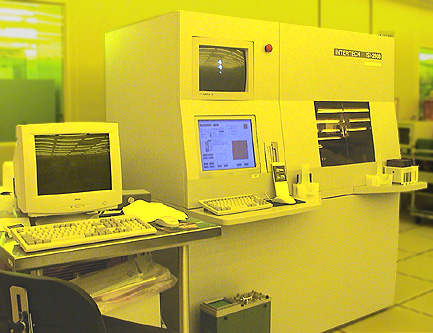
\includegraphics[width=\MachinePictureWidth]{pictures_machines/mask_maker.png}
\end{minipage}\begin{minipage}[H]{\MachineTextMiniPageWidth}
	\begin{tabular}{|p{3cm}|p{7cm}|}
		\hline
		Laser Source &
		\makecell[l]{
			Helium-Cadmium blue laser (20 mW) \\
			5000 hours life
		} \\
		\hline
		X - Y Stage &
		Laser Interferometer Stage \\
		\hline
		Maximum Writing Area &
		150 mm x 150 mm (6" x 6") \\
		\hline
		Laser Spot Size &
		0.7\um \\
		\hline
		Minimum Feature Size &
		1.5\um \\
		\hline
		Overlay Accuracy &
		0.3\um \\
		\hline
		Maximum Butting Error &
		0.3\um \\
		\hline
		Line Uniformity &
		$\pm 0.1 \mu m$ \\
		\hline
		Wring Grid &
		\makecell[l]{
			\tabitem 0.1\um \\
			\tabitem 0.2\um \\
			\tabitem 0.25\um \\
			\tabitem 0.5\um
		} \\
		\hline
		Writing Speed &
		\makecell[l]{
			\tabitem 1.28 $\frac{mm^2}{sec}$ @ 0.5\um grid \\
			\tabitem 0.64 $\frac{mm^2}{sec}$ @ 0.25\um grid
		} \\
		\hline
		Writing Method &
		Raster Scanning, width of swath 256\um \\
		\hline
		Depth of Focus &
		1.8\um \\
		\hline
	\end{tabular}
\end{minipage}

\subsection{ASML Stepper (PHT-S1)}\label{lithography_machine}
\WaferClean\WaferSemiClean

\begin{minipage}[H]{\MachinePictureWidth}
	\includegraphics[width=\MachinePictureWidth]{pictures_machines/litho_stepper.png}
\end{minipage}\begin{minipage}[H]{0.5\textwidth}
\begin{tabular}{|c|c|}
\hline
Light source illumination &
i-line (365 nm) \\
\hline
Resolution &
0.5\um \\
\hline
Maximum writing area &
$\pm 0.1 \mu m (3 \sigma)$ \\
\hline
Wafer size &
4" or 6" \\
\hline
Field size &
\makecell{15 mm x 15 mm or \\
10 mm x 10 mm (on wafer)} \\
\hline
Reduction ratio &
5:1 \\
\hline
Photomask size &
5" square \\
\hline
\end{tabular}
\end{minipage}
\subsection{DRIE Etcher \#1 (DRY-Si-1)}\label{dry_DRIE_etcher}
\WaferClean

\begin{minipage}[H]{\MachinePictureWidth}
	\includegraphics[width=\MachinePictureWidth]{pictures_machines/dry_DRIE.png}
\end{minipage}\begin{minipage}[H]{0.5\textwidth}
\begin{tabular}{|c|c|}
\hline
Gases available
&
C4F8, SF6, O2, N2, He \& Ar \\
\hline
RF power source
&
\makecell{1x 1000W(max) at 13.56MHz for Coil electrode,\\
1x 300W(max) at 13.56MHz for Platen electrode} \\
\hline
Electrode coolant system
&
5 to 30 \degreesC \\
\hline
High speed turbo molecular pump
&
\makecell{pumping speed of 1000 L/s at 36000 rpm \\
Fully automatic loadlock transfer system} \\
\hline
Substrate size
&
4" wafer \\
\hline
\end{tabular}

\underline{Silicon etch}

\begin{tabular}{|c|c|}
\hline
Minimum Line/Space
&
0.5 \um
\\
\hline
Low Rate Silicon Etch E/R
&
From 50nm/cycle \\
\hline
Normal Rate Silicon Etch E/R
&
Up to 2 \um/min\\
\hline
Selectivity to Photoresist
&
>50:1 \\
\hline
Selectivity to Oxide
&
>80:1 \\
\hline
Uniformity
&
7\percent \\
\hline
\end{tabular}
\end{minipage}
\subsection{Buehler Polisher (CMP-4)}\label{cmp_machine_semi_clean}
\WaferSemiClean
\begin{minipage}[H]{\MachinePictureWidth}
	\includegraphics[width=\MachinePictureWidth]{pictures_machines/silicon_polisher.png}
\end{minipage}\begin{minipage}[H]{0.5\textwidth}
\begin{itemize}
	\item Polished for
	\begin{itemize}
		\item Silicon
		\item Silicon Oxide 
		\item Silicon Nitride
	\end{itemize}
	\item $>5mm^2$ to 4" wafer size
	\item 100-800\um wafer thickness
\end{itemize}
\end{minipage}

\newpage
\subsection{Buehler Polisher (CMP-5)}\label{cmp_machine_unclean}
\WaferNonStandard

\begin{minipage}[H]{\MachinePictureWidth}
	\includegraphics[width=\MachinePictureWidth]{pictures_machines/copper_polisher.png}
\end{minipage}\begin{minipage}[H]{0.5\textwidth}
\begin{itemize}
	\item Polished for
	\begin{itemize}
		\item Copper
		\item Carbon nano tubes
		\item Silicon
		\item Silicon Oxide 
		\item Silicon Nitride
	\end{itemize}
	\item $>5mm^2$ to 4" wafer size
	\item 100-800\um wafer thickness
\end{itemize}
\end{minipage}
\subsection{Trion RIE Etcher (DRY-Trion)}\label{nitride_etch_machine}
\WaferSemiClean

\begin{minipage}[H]{\MachinePictureWidth}
	\includegraphics[width=\MachinePictureWidth]{pictures_machines/nitride_etcher.png}
\end{minipage}\begin{minipage}[H]{0.5\textwidth}
	\begin{tabular}{|c|c|}
		\hline
		Gases available &
		$CHF_3$, $SF_6$, $O_2$, $CF_4$, Ar, $N_2$, He and $H_2$ \\
		\hline
		ICP power source &
		600W (max) at 13.56MHz \\
		\hline
		RF power source &
		600W (max) at 13.56MHz \\
		\hline
		Electrode coolant system &
		0 to 30\degreesC \\
		\hline
		Substrate size &
		4", up to 3 wafers per run or specimens \\
		\hline
		Silicon Dioxide Etch &
		\~ 50 nm/min \\
		\hline
		Silicon Nitride Etch &
		\~ 85 nm/min \\
		\hline
	\end{tabular}
\end{minipage}


\subsection{Diffusion Furnace (DIF-A1, DIF-C1 to DIF-C4, DIF-D1 to DIF-D4, DIF-F1)}\label{diffusion_furnace_machine}
\WaferClean\WaferSemiClean\WaferNonStandard

	\begin{tabular}{|p{4cm}|p{8cm}|}
		\hline
		Operating temperature &
		400 to 1150 \degreesC \\
		\hline
		Processing &
		\makecell[l]{
			\tabitem Dry \& Wet Oxidation with TCE\\
			\tabitem N/P diffusion \\
			\tabitem Forming Gas annealing and Drive in
		} \\
		\hline
	\end{tabular}

\newpage
\subsection{LPCVD (CVD-A2 to CVD-A4, CVD-B1 to CVD-B4, CVD-F2 to CVD-F4)}\label{lpcvd_machine}
\WaferClean\WaferSemiClean (\textbf{CVD-B1: GaN only})

\begin{minipage}[H]{\MachinePictureWidth}
	\includegraphics[width=\MachinePictureWidth]{pictures_machines/poly_deposit.png}
\end{minipage}\begin{minipage}[H]{0.5\textwidth}
Each deposition has its programmed flow of gases compositions, temperature and pressure

\begin{mdframed}
ASM LB45  LPCVD Furnace:
\begin{itemize}
	\item Polysilicon
	\item Amorphous silicon
	\item Silicon Germanium
	\item Silicon Nitride
	\item Low Temperature Oxide (LTO)
	\item Phosphorous Silicon Glass (PSG)
\end{itemize}
\end{mdframed}\begin{mdframed}
Flokal LPCVD Furnace:
\begin{itemize}
	\item Polysilicon
	\item Amorphous silicon
	\item Silicon Nitride
	\item Low Stress Silicon Nitride
	\item LTO
	\item PSG
\end{itemize}
\end{mdframed}

\end{minipage}
\subsection{Poly Etcher (DRY-Poly)}\label{poly_etcher_machine}
\WaferClean\WaferSemiClean

\begin{minipage}[H]{\MachinePictureMiniPageWidth}
	\includegraphics[width=\MachinePictureWidth]{pictures_machines/poly_etcher.png}
\end{minipage}\begin{minipage}[H]{\MachineTextMiniPageWidth}
	\begin{tabular}{|p{3cm}|p{8cm}|}
		\hline
		Remark &
		For Semi-Clean process, please contact NFF technicians. \\
		\hline
		Gases available &
		$H Br$, $Cl_2$, $O_2$, $N_2$, $He$ and $Ar$ \\
		\hline
		RF power source &
		\makecell[l]{
			\tabitem 1x 1000W(max) at 13.56MHz for Coil electrode \\
			\tabitem 1x 300W(max)  at 13.56MHz for Platen electrode
		} \\
		\hline
		Electrode coolant system &
		20 \degreesC \\
		\hline
		High speed turbo molecular pump &
		\makecell[l]{
			\tabitem Pumping speed of 1000 L/s at 36000 rpm \\
			\tabitem Fully automatic loadlock transfer system
		} \\
		\hline
		Substrate size &
		4” single wafer \\
		\hline
	\end{tabular}

	\underline{Polysilicon etch}

	\begin{tabular}{|p{5cm}|p{6cm}|}
		\hline
		Minimum line/space &
		0.5\um \\
		\hline
		Low rate polysilicon etch E/R &
		\~ 90 nm/min \\
		\hline
		Selectivity to oxide &
		13:1 \\
		\hline
		Selectivity to photoresist &
		12.5:1 \\
		\hline
		Uniformity &
		5 \% \\
		\hline
	\end{tabular}

	\underline{Normal rate polysilicon etch}

	\begin{tabular}{|p{5cm}|p{6cm}|}
		\hline
		E/R &
		>180 nm/min \\
		\hline
		Selectivity to photoresist &
		2.5:1 \\
		\hline
		Uniformity &
		5\% \\
		\hline
	\end{tabular}
\end{minipage}
\newpage
\section{Resists}
\input{resists_overview.tex}

\newpage
\listoffootnotes \cleardoublepage

\end{document}
